%%
%
% ARQUIVO: main.tex
%
% VERSÃO: 1.0
% DATA: Maio de 2016
% AUTOR: Coordenação de Trabalhos Especiais SE/8
% 
%  Arquivo tex principal do documento de Projeto de Fim de Curso (PFC).
%  Este arquivo SÓ PRECISA SER MODIFICADO NA PARTE DE CONTEÚDO:
%
%    a. colocar um \include{•} para cada capítulo do documento de PFC.
%
%

% -----
% CLASSE DO DOCUMENTO DE PFC
% -----
\documentclass{pfc}

% -----
% PACOTES LATEX USADOS NO DOCUMENTO DE PFC
% -----
\usepackage[brazilian]{babel}
\usepackage[utf8]{inputenc}
\usepackage[T1]{fontenc}

\usepackage{amsmath}
\usepackage{graphicx}
\usepackage{tabularx}
\usepackage{float}
\usepackage{color}
\usepackage{amsfonts,amssymb}
\usepackage[authoryear]{natbib}

\usepackage{enumitem}
\usepackage{rotating}
\usepackage{lipsum}
\usepackage{lastpage}
\usepackage{stringstrings}
\usepackage{pgffor}
\usepackage{pdftexcmds}
\usepackage{subfigure}

\usepackage{pgfgantt}
\usepackage{xcolor}
\usepackage[utf8]{inputenc}
\usepackage{import}
\usepackage{svg}


\usepackage{tikz}
\usepackage{float}
\usepackage{blindtext}

\definecolor{verylightgray}{RGB}{220,220,220}
\definecolor{groupblue}{RGB}{51,102,254}
\definecolor{linkred}{RGB}{165,0,33} 
\definecolor{silver}{RGB}{192,192,192} 

\usepackage{listings}

 \lstset{frame=tb,
  language=Python,
  basicstyle=\ttfamily,
  breaklines=true,
  showstringspaces=false,
  showspaces=false,
  columns=flexible,
  numbers=none,
  commentstyle=\color{dkgreen},
  tabsize=1
}

% -----
% MARGENS DO DOCUMENTO DE PFC
% -----
\usepackage{geometry}
\geometry{
	a4paper,
	total={210mm,297mm},
	left=25mm,
	right=25mm,
	top=25mm,
	bottom=30mm,
	textwidth=160mm,
	textheight=242mm,
	headheight=0mm,
	headsep=0mm,
}

% -----
% DECLARAÇÕES AUXILIARES PARA REFERÊNCIAS
%
%  Diferencia \citet e \citep de acordo com a NBR 10520:2002
% -----
\DeclareRobustCommand{\NATand}{;}
\DeclareRobustCommand{\NATetal}{et~al.}
\makeatletter
\renewcommand{\NAT@nmfmt}[1]{%
  \ifNAT@swa\expandafter\MakeUppercase
  \else\DeclareRobustCommand{\NATand}{ e}\expandafter\@firstofone\fi{{\NAT@up #1}}%
}
\makeatother

% -----
% AMBIENTE DE FIGURAS DE PFC
%
%  A classe do documento está configurada SOMENTE para figuras no formato EPS.
%  Logo, use PREFERENCIALMENTE este tipo de arquivo.
%
%    a. os arquivos das figuras devem estar no diretório 'img'
% -----
\graphicspath{{./img/}}

% -----
% INÍCIO DO DOCUMENTO DE PFC
% -----
\begin{document}

% -----
% PARTE PRÉ-TEXTUAL DE PFC
%
% Alterar o CONTEÚDO dos arquivos siglas.tex E pre-texto.tex
% -----
% ARQUIVO: dados-pfc.tex
%
% VERSÃO: 1.0
% DATA: Maio de 2016
% AUTOR: Coordenação de Trabalhos Especiais SE/8
% 
%  Arquivo tex com os dados acerca do documento de PFC e da apresentação.
%
%   nos campos que definem nomes (autor; orientador; co-orientador; membros da banca)
%   É PRECISO usar os COMANDOS LaTeX para acentuação, conforme abaixo:
%
%         \'a - á || \`a - à || \~a - ã || \^a - â 
%         \'e - é || \^e - ê || \'i - í 
%         \'o - ó || \~o - õ || \^o - ô 
%         \'u - ú || \"u - ü
%
%%

%%% AUTORES DO PFC (Nome completo)
% ---
%  aceita até 03 autores (de autorI até autorIII)
%    a. preencher sucessivamente a partir de autorI
%    b. REMOVER as definições não necessárias
% ---
\autorI{Rafael Lara Cardoso}
\autorII{Luana Marques Mello Pereira}
%\autorIII{Nome Completo do Terceiro Autor}

%%% POSTOS DOS AUTORES DO PFC
% ---
%  aceita os postos de até 03 autores (de postoautorI até postoautorIII)
%    a. preencher sucessivamente a partir de postoautorI (que deve ser o posto de autorI)
%    b. se o autorX É CIVIL, NÃO DEFINIR postoautorX (remover a linha de definição)
%    c. se o autorX É MILITAR, DEFINIR postoautorX com UMA das seguintes ALTERNATIVAS: Alu / 1 Ten / Cap
% ---
\postoautorI{Cap}
\postoautorII{1º Ten}

%%% TITULO DO PFCC
\titulo{POSICIONAMENTO PRECISO POR GNSS EM TEMPO REAL}

%%% DATA DA APRESENTAÇÃO (formato {dd}{Mmmmm}{aaaa})
\datadefesa{11}{Outubro}{2019}

%%% ORIENTADOR DO PFC
% ---
%  CAMPO 1: P (para Prof.); PA (para Profa.); ou qualquer coisa (inclusive VAZIO) - o que for escrito aparecerá no documento
%  CAMPO 2: Nome completo
%  CAMPO 3: D (para D.Sc.); P (para Ph.D.); M (para M.Sc.) ou qualquer coisa (inclusive VAZIO) - o que for escrito aparecerá no documento
%  CAMPO 4: Instituição (com "do / da")
% ---
\orientador{P}{Haroldo Antonio Marques}{D}{do IME}
%\orientador{PA}{Helo{\'i}sa Alves Silva Marques}{D}{do IME}

%%% CO-ORIENTADOR DO PFC
% ---
%  se não houver co-orientador, REMOVA ESTA LINHA
%  preenchimento idêntico a \orientador{}{}{}{}
% ---
\coorientador{PA}{Helo{\'i}sa Alves Silva Marques}{D}{do IME}

%%% NÚMERO DA ENTRADA DA BIBLIOTECA (pegar na Biblioteca do IME)
\biblioref{000.00}{x000x}

%%% PALAVRAS-CHAVES DO PFC
% ---
%  devem ser separadas por vírgula e É OBRIGATÓRIO ter pelo menos uma
% ---
\palavraschaves{GNSS, RTPPP, PPP-RTK, RTK/NTRIP, Plataformas Livres}

%%% OUTROS MEMBROS DA BANCA DO PFC
% ---
%  aceita até mais 05 membros (de membrobancaI até membrobancaV)
%    a. preencher sucessivamente a partir de membrobancaI
%    b. REMOVER as definições não necessárias
%
%  cada membro tem preenchimento idêntico a \orientador{}{}{}{}
% ---
\membrobancaI{P}{Leonardo Castro de Oliveira}{D}{do IME}
\membrobancaII{}{Maj Stefano Sampaio Suraci}{M}{do IME}
%%
%
% ARQUIVO: pre-texto.tex
%
% VERSÃO: 1.0
% DATA: Maio de 2016
% AUTOR: Coordenação de Trabalhos Especiais SE/8
% 
%  Arquivo tex para a criação da parte pré-textual do documento de Projeto de Fim de Curso.
%
%%


% -----
% PÁGINA DE CAPA DO DOCUMENTO DE PFC
% -----
\makecapa

% -----
% PÁGINA DE TÍTULO DO PFC
% -----
\prepareadvisors
\maketitle

% -----
% PÁGINA DE CRÉDITOS DO DOCUMENTO DE PFC
% -----
\makecredits

% -----
% PÁGINA DE FOLHA DE ASSINATURAS
% -----
\preparemembers
\approvalpage

% -----
% PÁGINA DE DEDICATÓRIA (OPCIONAL, ie. pode remover toda a página)
% -----
%%% DEDICATÓRIA - PREENCHER...
\dedicatoria{%
À Deus que sempre guia nossos passos pelo melhor caminho; Às nossas famílias que sempre estiverem presentes para apoiar-nos e Ao Instituto Militar de Engenharia, alicerce de nossa formação e aperfeiçoamento profissional.}%
\makededication

% -----
% PÁGINA DE AGRADECIMENTOS (OPCIONAL, ie. pode remover toda a página)
% -----
%%% AGRADECIMENTOS - PREENCHER...
\agradecimentos{%
É chegado ao fim de um ciclo, o qual se iniciou há muitos anos atrás, por meio de constantes desafios e conquistas. Sendo assim, agradecemos aos apoiadores dessa trajetória, nossa família, alicerce fundamental de vida e todos os professores envolvidos na caminhada, especialmente os nossos orientadores Profª Dra. Heloísa Alves Silva Marques e Profº Dr. Haroldo Antônio Marques. Gostaríamos de agradecer também ao 2º Ten Marco e ao Cap R1 Eduardo, que nos prestaram grande apoio durante as atividades práticas desse projeto estando sempre disponíveis nos momentos que foram necessários.}%
\makethanks

% -----
% PÁGINA DE EPÍGRAFE (OPCIONAL, ie. pode remover toda a página)
% -----
%%% EPÍGRAFE - PREENCHER...
\epigrafe{%
Não existe triunfo sem perda, não há vitória sem sofrimento e não há liberdade sem sacrifício.
}%
\autorepigrafe{%    %% Se não tem autor, coloque "Anônimo"
J. R. R. Tolkien
}%
\makeepigraph

% -----
% PÁGINA DE SUMÁRIO
% -----
\tableofcontents

% -----
% PÁGINAS DE LISTAS DE FIGURAS E DE TABELAS
% se a Dissertação não possui figuras e/ou tabelas, REMOVA O COMANDO CORRESPONDENTE
% -----
\listoffigures
%\listoftables

% -----
% PÁGINA DE LISTA DE SIGLAS
% se a Dissertação não possui siglas, REMOVA TODA A PÁGINA
% -----
%%% SIGLAS - PREENCHER...

\acronimo{GPS}{Global Positioning System}
\acronimo{DGPS}{Differential Global Positioning System}
\acronimo{GNSS}{Global Navigation Satellite System}
\acronimo{PPP}{Precise Point Positioning}
\acronimo{RTPPP}{Real-Time Precise Point Positioning}
\acronimo{PPP-RTK}{Precise Point Positioning Real-Time Kinematic}
\acronimo{IAG}{International Association of Geodesy}
\acronimo{IGS}{International GNSS Service}
\acronimo{RTCM}{Radio Technical Commission for Maritime Services}

\listofnicks


% -----
% PÁGINA DE LISTA DE ABREVIATURAS
% se a Dissertação não possui abreviaturas ou símbolos, REMOVA TODA A PÁGINA
% -----
%%% ABREVIATURAS
%\abreviatura{iid}{Independente e Identicamente Distribuído}
%\abreviatura{MA}{\textit{Moving Average}}


%%% SÍMBOLOS - PREENCHER...
%\simbolo{$\mu$}{média}
%\simbolo{$\gamma$}{covariância}
%\simbolo{$\rho$}{correlação}


%\listofsymbols

% -----
% PÁGINA DE RESUMO
% -----
%%% RESUMO - PREENCHER...
\resumo{%
O presente relatório visa apresentar as etapas do projeto envolvendo posicionamento preciso em tempo real por GNSS utilizando ferramentas livres e aplicação dos seguintes métodos: Método Relativo Cinemático (RTK),Posicionamento por Ponto Preciso em Tempo Real (RTPPP) e integração de RTK com PPP, denominado PPP-RTK. O método RTK é bem conhecido nas áreas de engenharia e, em geral, utiliza-se a transmissão de correções em tempo real via link de rádio, contudo, atualmente é possível utilizar a transmissão de dados via RTCM utilizando protocolo NTRIP. O método RTPPP é relativamente novo e requer correções de órbitas (posição dos satélites) e relógios em tempo real, o que pode ser obtido via protocolo NTRIP utilizando, por exemplo, os serviços gratuitos do IGS. Ao receber as correções em tempo real de uma rede de estações GNSS, o método RTPPP permite fixar as ambiguidades da fase da portadora e passa a ser denominado PPP-RTK. Esses métodos (RTPPP e PPP-RTK) atualmente não são totalmente operacionais, haja vista que a maioria dos receptores GNSS não estão preparados para a recepção de dados em tempo real, além de outras questões, como por exemplo, a disponibilidade de internet em diversas regiões do Brasil. Uma possibilidade é utilizar serviços pagos, tal como o OminiSTAR-XP e Trimble-RTX, os quais enviam correções em tempo real a partir de satélites geoestacionários. Dessa forma, o objetivo desse projeto final de curso é aplicar os métodos RTK, RTPPP e PPP-RTK utilizando plataformas livres e verificar a qualidade posicional visando o monitoramento em tempo real, o qual será útil para monitorar frotas, estimar posições de embarcações e aeronaves, monitorar estruturas, entre outras aplicações. 
}%
\makeresumo

\abstract{%
This project aims to present the design steps involving GNSS real-time accurate positioning using free tools and applying the following methods: Relative Kinematic Method (RTK), Real-Time Precise Point Positioning (RTPPP) and integration of RTK with PPP, called PPP-RTK. The RTK method is well known in the engineering field and radio link real-time correction is generally used, however it is currently possible to use data transmission via RTCM using NTRIP protocol. The RTPPP method is relatively new and requires real time orbit (satellite position) and clock correction, which can be obtained via the NTRIP protocol using, for example, free IGS services. When receiving real-time corrections from a network of GNSS stations, the RTPPP method allows the carrier phase ambiguities to be fixed and is renamed PPP-RTK. These methods (RTPPP and PPP-RTK) are currently not fully operational, as most GNSS receivers are not prepared for real-time data reception, as well as other issues such as internet availability in various regions of Brazil. One possibility is to use paid services, such as OminiSTAR-XP and Trimble-RTX, which send real-time corrections from geostationary satellites. Thus, the purpose of this final course project is to apply RTK, RTPPP and PPP-RTK methods using free platforms and verify positional quality for real-time monitoring, which will be useful for monitoring fleets, estimating vessel and aircraft positions. , monitor structures, among other applications.
}%
\makeabstract


\parindent 0.75cm

% -----
% PARTE DE CONTEÚDO DE PFC
%
%  Escrever cada capitulo do documento de PFC em um arquivo .tex separado.
%  Adicionar os arquivos .tex ao documento com comando \include{•}
% -----
\chapter{Introdução}

Os Sistemas de Navegação Global por Satélite, do inglês \textit{Global Navigation Satellite Systems (GNSSs)}, possibilitam a estimativa da posição geográfica de um ponto em qualquer lugar da superfície terrestre e em suas proximidades. Suas aplicabilidades vão muito além do mapeamento, como sincronização de relógios ao redor do globo, navegação, segurança, agricultura de precisão, aviação civil, meio ambiente, forças armadas, entre outras. \citep{liu2018real} \citep{monico2008}.

Os sistemas de navegação por satélites atualmente disponíveis, como GPS, GLONASS, Galileu, Beidou-Compass estão em constante processo de evolução e modernização, englobando os seguimentos de controle e espacial com a transmissão de sinais modernizados no qual se espera melhorias na acurácia posicional e na integridade dos sistemas.Os métodos de posicionamento por GNSS são aprimorados com o passar dos anos em função da evolução tecnológica e da demanda por maior acurácia e versatilidade.

Os métodos de posicionamento por GNSS, basicamente, podem ser classificados em \textit{posicionamento absoluto}, quando as coordenadas estão associadas diretamente ao geocentro e \textit{posicionamento relativo}, quando as coordenadas são determinadas com relação a um referencial materializado por um ou mais vértices com coordenadas conhecidas \citep{monico2008}.

Neste Projeto Final de Curso, três métodos serão aplicados os métodos: o RTPPP (\textit{Real Time Precise Point}), RTK (\textit{Real Time Kinematic}) e o PPP-RTK (integração RTPPP e RTK).


O RTPPP envolve a aplicação de PPP (Posicionamento Por Ponto Preciso) em Tempo real) e requer somente um receptor ao nível do usuário, diferente do RTK, que requer observações e correções de uma base.  Ao utilizar-se de conexão com internet, com um software de processamento em tempo real, é possível receber as órbitas transmitidas dos satélites bem como a correção das órbitas e relógios. \citet{marques2014ppp} ressaltam que o método RTPPP encontra-se em desenvolvimento para aplicação em larga escala até nos dias atuais e cita melhorias que podem ser buscadas, tais como a diminuição no tempo de convergência e a utilização da solução fixa de ambiguidades ao invés da solução float, o que é factível no posicionamento relativo. A acurácia esperada do método RTPPP é na ordem decimétrica \citep{lima}.

No caso do RTK, diversos trabalhos têm mostado a potencialidade do método para aplicações em tempo real, onde se pode destacar o RTK em rede com aplicações de estações virtuais \citep{daniele}. O padrão de transmissão no RTK, em geral, utiliza o formato RTCM com envio a partir de link de rádio, contudo, com o desenvolvimento do protocolo NTRIP, diversos receptores na atualidade permitem a inserção de chips com tecnologia GSM e acesso à internet de tal forma que se pode utilizar o protocolo NTRIP e a recepção de dados de estações de uma rede de monitoramento contínuo. A utilização de tal protocolo no RTK tem levado a comunidade usuária no Brasil à classificar o método como RTK/NTRIP.


Nesse trabalho de PFC foram aplicados os métodos RTPPP, PPP-RTK e RTK com envio de dados a partir de link de radio e também via NTRIP. Para aplicação dos métodos foi utilizado o receptor GR-5 da Topcon, sendo este equipamento recém chegado na seção de ensino 6 do IME, o que demandou considerável tempo do alunos para o entendimento e treinamento com o método. Para aplicação do RTPPP foi utilizado o software BNC disponibilizado pelo centro Alemão BKG e a solução foi realizada para estação estática da RBMC, bem como com conexão do software no receptor GR-5 via porta serial. O método PPP-RTK foi realizado utilizando o software PPP-Wizard disponibilizado pelo CNES (Centre National d'Études Spatiales) da França, sendo que este permite receber diversas informações da rede mundial do IGS e possibilita a solução fixa das ambiguidades. 
Os resultados obtidos nos levantamentos em campo foram analisados a partir da série temporal de estimativa de precisões, bem como dos valores de Erro Médio Quadrático (EMQ), ao comparar a solução em tempo real com solução pós-processada ou com coordenadas oficiais das estações. 




\section{Motivação}
\label{motivacao}
\noindent

A motivação do trabalho surge a partir de algumas questões e demandas. Como realizar um posicionamento por GNSS, em tempo real, utilizando os métodos de posicionamento RTPPP, RTK e PPP-RTK? Quais são as ferramentas livres na atualidade e como utilizar para a aplicações desses métodos? A acurácia posicional proporcionada pelos métodos de posicionamento em tempo real atende a demanda por levantamentos precisos e de navegação? A busca pelas respostas instiga o projeto

O crescimento da demanda por serviços de posicionamento GNSS no Brasil e no mundo aumenta a necessidade de documentação técnica a respeito do tema. A possibilidade de ter normas e padronizações a respeito do tema é interessante pois possibilita o uso de forma facilitada dos referidos métodos em diversas aplicações, tais como:

\begin{itemize}
    \item Monitoramento de frotas em tempo real;
    \item Monitoramento da posição de agentes de segurança pública em operações;
    \item Utilização pelas Forças Armadas para monitoramento em operações;
    \item Georreferenciamento de imóveis rurais;
    \item Levantamento de coordenadas para construção civil;
    \item Obtenção de coordenadas precisas de maneira eficiente para construção de rodovias;
    \item Utilização em qualquer aplicação que requeira métodos de posicionamento em tempo real com precisão centimétrica, etc.
\end{itemize}



Em 2013 foi publicada no Brasil a ''Norma Técnica para georreferenciamento de Imóveis Rurais'' \citep{ibge_imoveis}. Essa norma especifica os métodos de posicionamento que podem ser utilizados para o georreferenciamento de imóveis rurais no Brasil. Entre os métodos previstos estão o PPP em tempo real e RTK em rede (RTK/NTRIP), métodos que este trabalho se propõe a avaliar.

De acordo com o decreto nº 4.449, de 30 de outubro de 2002, e o decreto 9.311, de 15 de março de 2018, os proprietários de imóveis rurais de 25 a 100 hectares possuem até 20/11/2023 para apresentarem, junto ao governo federal, os georreferenciamentos de suas respectivas propriedades; os proprietários de imóveis com área inferior a 25 hectares possuem até 20/11/2025.

Embora os referidos decretos estejam em vigor e o ''Manual Técnico de Posicionamento: georreferenciamento de imóveis rurais'' publicado, é possível verificar a pouca utilização dos métodos de posicionamento por GNSS pelos grupos e empresas. Muitas das vezes pela resistência às novas tecnologias, falta de equipamento adequado e conhecimento. Dessa forma, busca-se disseminar as técnicas estudadas e apresentar de maneira confiável as acurácias que podem ser obtidas com cada uma.

Além da área de posicionamento para georreferenciamento de imóveis rurais existe também o interesse nesse tipo de posicionamento em empresas diversas de transporte e no setor de segurança pública. Uma empresa com frota de transporte rodoviário pode, utilizando os métodos aqui estudados, monitorar suas viaturas em tempo real com precisão decimétrica ou centimétrica de maneira confiável.

Indo além, órgãos de segurança pública e Forças Armadas podem rastrear, em tempo real, com a precisão citada, diversos escalões, tais como:
\begin{itemize}
    \item Pelotão em atividade de Garantia da Lei e da Ordem;
    \item Viaturas de transporte de suprimento ou pessoal;
    \item Barcos e embarcações diversas para transporte de suprimento ou pessoal;
    \item Grupos de agentes de segurança pública em atividades diversas;
    \item Viaturas das Polícias Militares;
    \item Monitoramento da frota de transporte público de determinada cidade; etc
\end{itemize}

Por fim, pela carência de literatura na área no Brasil, tais métodos carecem de normas técnicas e manuais que possam apresentar os passos necessários para realizar na prática tais métodos de posicionamento. Suprir essa carência é essencial para a disseminação do conhecimento. 


\section{Objetivo}
\noindent
O presente Projeto Final de Curso tem como objetivo geral:

Aplicar e avaliar a acurácia de levantamento a partir dos métodos de posicionamento em tempo real RTPPP, RTK e PPP-RTK fazendo uso de receptores GNSS modernos, dados de redes geodésicas de monitoramento contínuo e plataformas computacionais livres.


Objetivos Específicos:
\begin{itemize}
    \item Treinamento com o par de receptores GR-5 da Topcon adquirido recentemente pelo IME;
    \item Levantamento RTK padrão utilizando a comunicação via link de rádio;
    \item RTPPP com o BNC/BKG em estação estática da RBMC;
    \item RTPPP com o BNC/BKG e conexão com o receptor GR5 a partir da porta serial;
    \item PPP-RTK fazendo uso do aplicativo PPP-Wizard fornecido pelo CNS;
    \item Avaliação de acurácia dos levantamentos realizados.
\end{itemize}



\chapter{Fundamentação Teórica}
\label{chap:fundament}

\section{Métodos de posicionamento GNSS}
\noindent

De acordo com \cite{monico2008}, posicionamento diz respeito à determinação da posição de objetos com relação a um determinado referencial. Neste contexto, o posicionamento pode ser dividido em: \textit{Absoluto} e \textit{Relativo}. Absoluto, quando as coordenadas estão diretamente associadas ao geocentro; e Relativo, quando são determinadas em relação a um referencial materializado por um ou mais vértices com coordenadas conhecidas. Outra classificação que pode ser feita é quanto ao movimento do objeto a ser posicionado em relação ao referencial. Pode-se dividir em \textit{cinemático}, quando o objeto está em movimento em relação ao referencial ou \textit{estático} quando esse está em repouso.

Ainda não existe uma terminologia padrão para os métodos de posicionamento GNSS junto a comunidade científica, desta forma, neste PFC será adotada a classificação de \cite{monico2008}:
\begin{itemize}
    \item Posicionamento absoluto;
    \item Posicionamento relativo;
    \item Posicionamento com DGPS.
\end{itemize}

Serão aplicados no presente trabalho os métodos de RTPPP e PPP-RTK que enquadram-se em posicionamento absoluto e o método de RTK que é classificado como posicionamento relativo.

\section{Protocolo de transmissão de dados GNSS}
\noindent

Para realizar os métodos de posicionamento GNSS por vezes são necessários protocolos de transmissão que possibilitem a correta comunicação entre as peças envolvidas no método; o RTCM é um padrão empregado em operações com GPS envolvendo posicionamento nos modos DGPS e RTK.

O padrão RTCM foi desenvolvido pela \textit{Radio Technical Commission for Maritime Services}. Este padrão de formato de dados é utilizado para a transmissão de informações entre uma estação de referência e outra remota, geralmente em movimento, possibilitando posicionamento em tempo real.

Na área de navegação e posicionamento, o padrão mais comum é aquele conhecido como padrão SC-104 (geralmente chamado apenas de padrão RTCM). Em meados da década de 80, a RTCM estabeleceu um comitê especial, de número 104. O objetivo inicial deste comitê especial era o de projetar um formato padrão que permitisse a transmissão de informações, das mais diversas, relacionadas com o emprego da tecnologia GPS. Este objetivo se expandiu e atualmente o formato possibilita a transmissão de informações para outros sistemas GNSS (tais com o GLONASS) \citep{Navipedia2019}.


\section{Posicionamento Por Ponto Preciso (PPP)}
\noindent

Com o intuito de entender melhor a base para os métodos de RTPPP e PPP-RTK, será tratado a respeito do método PPP. O método do PPP se utiliza  de efemérides precisas e correções de relógios dos satélites. Tal termo foi utilizado primeiramente por \cite{heroux1995gps}. Essa metodologia de posicionamento se utiliza, assim como as outras, de três componentes: as observações; os modelos de correção; e o processo de ajustamento \citep{cunha2016_PPP}. O seu ganho de precisão em relação ao \textit{Posicionamento por Ponto Absoluto} é a utilização de observações e métodos para correção das observações. As observações utilizadas englobam as efemérides e correções dos relógios dos satélites. A utilização dessas observações combinada ao modelos de correção e ajustamento proporciona ao PPP uma precisão centimétrica. O PPP divide-se em duas fases:

\begin{enumerate}
    \item Centrais de análise recebe os dados de controle de GNSS e cria produtos precisos;
    \item Os produtos de elevada precisão são utilizados para processar os dados coletados pelo receptor GNSS.
\end{enumerate}

É importante salientar que para a realização do PPP é necessário um receptor GNSS de dupla frequência. \cite{cunha2016_PPP} cita \cite{kouba2001precise} ao caracterizar o modelo tradicional de PPP:
\begin{itemize}
    \item Combinação de observações de dupla frequência da pseudodistância e da fase da portadora para criar uma observação \textit{ion-free} (IF);
    \item Implementação de um filtro sequencial para o procedimento de ajuste;
    \item Determinação do atraso troposférico zenital húmido como uma incógnita adicional;
    \item Utilização de modelos para estimar o valor das restantes fontes de erro.
\end{itemize}


\subsection{Modelo matemático do PPP}
\noindent

A seguir será apresentado o modelo funcional do PPP. Utilizando dados de um receptor GNSS de dupla frequência, as equações de pseudodistância e fase da onda portadora parametrizada com a aplicação da combinação ion-free (IF) podem ser escritas da seguinte forma \citep{marques2012ppp}:

\begin{equation}
    \label{eq:PD}
    PD_{IF_r}^{s}=\rho_r^s+c.(dt_r(t_r)+dt^s(t^t))+m_f.Zwd+\varepsilon_{PD_r^{s}}
\end{equation}

\begin{equation}
    \label{eq:lambda}
    \lambda_{IF}.\phi_{IF_r}^{s}=\rho_r^s+c.(dt_r(t_r)-dt^s(t^t))+\lambda_{IF}.N_{IF}+m_f.Zwd+\varepsilon_{\phi_r^{s}}
\end{equation}

Nas equações \ref{eq:PD} e \ref{eq:lambda} tem-se que:
\begin{itemize}
    \item $PD_{IF_r}^{s}$ - pseudodistância da \textit{ion-free} (metros);
    \item $\lambda_{IF}.\phi_{IF_r}^{s}$ - fase da \textit{ion-free} (metros);
    \item $\rho_r^s$ - distância geométrica entre receptor r e o satélite s;
    \item $dt_r(t_r)$ - erro do relógio do receptor no instante de recepção $t_r$;
    \item $dt^s(t^t)$ - erro do relógio do receptor no instante de recepção $t^t$
    \item $N_{IF}$ - ambiguidade da \textit{ion-free};
    \item Zwd - atraso troposférico úmido na direção do zênite;
    \item $m_f$ - função de mapeamento do Zwd para a direção receptor-satélite; e
    \item $\varepsilon_{PD_r^{s}}$ e $\varepsilon_{\phi_r^{s}}$ - os erros aleatórios e não modelados nas equações \textit{ion-free} de pseudodistância e fase.
\end{itemize}

As equações \ref{eq:PD} e \ref{eq:lambda} apresentam modelos não lineares e a equação linearizada considerando um receptor \textit{r} e o satélite $s_i$, pode ser escrita como \citep{marques2014ppp}:
\begin{equation}
\label{lin_ppp}
E
\begin{Bmatrix}
\begin{bmatrix}
\Delta PD_{IF_r}^{s_i}\\
\Delta \lambda_{IF}.\phi_{IF_r}^{s_i}
\end{bmatrix}
\end{Bmatrix}
=AX=
\begin{bmatrix}
-\frac{X^{s_i}-X^0_r}{(\rho^{s_i}_r)^0} & -\frac{Y^{s_i}-Y^0_r}{(\rho^{s_i}_r)^0}& -\frac{Z^{s_i}-Z^0_r}{(\rho^{s_i}_r)^0} & 1 & M_f & 0\\
-\frac{X^{s_i}-X^0_r}{(\rho^{s_i}_r)^0} & -\frac{Y^{s_i}-Y^0_r}{(\rho^{s_i}_r)^0}& -\frac{Z^{s_i}-Z^0_r}{(\rho^{s_i}_r)^0} & 1 & M_f & \lambda_{IF}
\end{bmatrix}
\begin{bmatrix}
\Delta X_r\\
\Delta Y_r\\
\Delta Z_r\\
\Delta c.dt_r\\
Z_{wd}\\
N^{s_i}_{IF}
\end{bmatrix}
\end{equation}

Na equação \ref{lin_ppp}:
\begin{itemize}
    \item $\Delta PD_{IF_r}^{s_i}$ - diferença entre a pseudodistância observada e a calculada (vetor L para pseudodistância);
    \item $\Delta \lambda_{IF}.\phi_{IF_r}^{s_i}$ - diferença entre a fase observada e a calculada (vetor L para fase);
    \item $(\rho^{s_i}_r)^0$ - distância geométrica calculada em função dos parâmetros aproximados; e
    \item E\{.\} - representa o operador de esperança matemática.
    \item Os termos $\Delta X_r$, $\Delta Y_r$, $\Delta Z_r$, $dt_r$, $Z_{wd}$ e $N_{IF}$ são as correções aos parâmetros incógnitos, ou seja, as coordenadas da estação, erro do relógio do receptor, troposfera e ambiguidade.
\end{itemize}


\section{Posicionamento Por Ponto Preciso em tempo real (RTPPP)}

\begin{figure}[H]
\centering
% ---
% Taken from https://cremeronline.com/LaTeX/minimaltikz.pdf
\tikzstyle{block} = [rectangle, draw, fill=white, text width=6em, text centered, rounded corners, node distance=2cm, minimum height=2em]
\tikzstyle{cloud} = [draw, ellipse,fill=white, node distance=2cm, minimum height=2em]
\fbox{
\begin{tikzpicture}
%\node[inner sep=0pt] (sat) at (0,0) {
\includegraphics[width=.15\textwidth]{satelite.png}};
    
\node[inner sep=0pt] (rec1) at (0,-10) [label=below:Receptor 1] {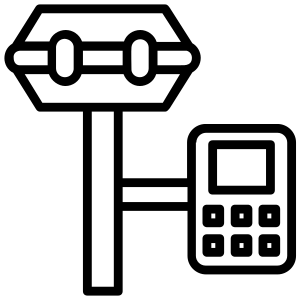
\includegraphics[width=.05\textwidth]{receiver.png}};
\node[inner sep=0pt] (rec2) at (2.5,-10) [label=below:Receptor 2] {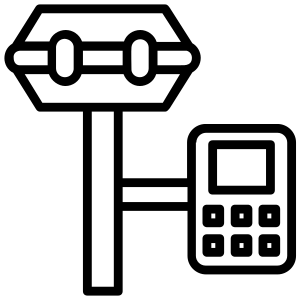
\includegraphics[width=.05\textwidth]{receiver.png}};
\node (recponto) at (5,-10) {...};
\node[inner sep=0pt] (recn) at (7.5,-10) [label=below:Receptor n] {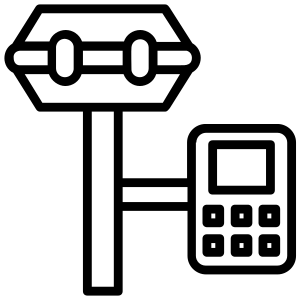
\includegraphics[width=.05\textwidth]{receiver.png}};


\node[inner sep=0pt] (laptop) at (5,-5) [label=left:Software BNC] {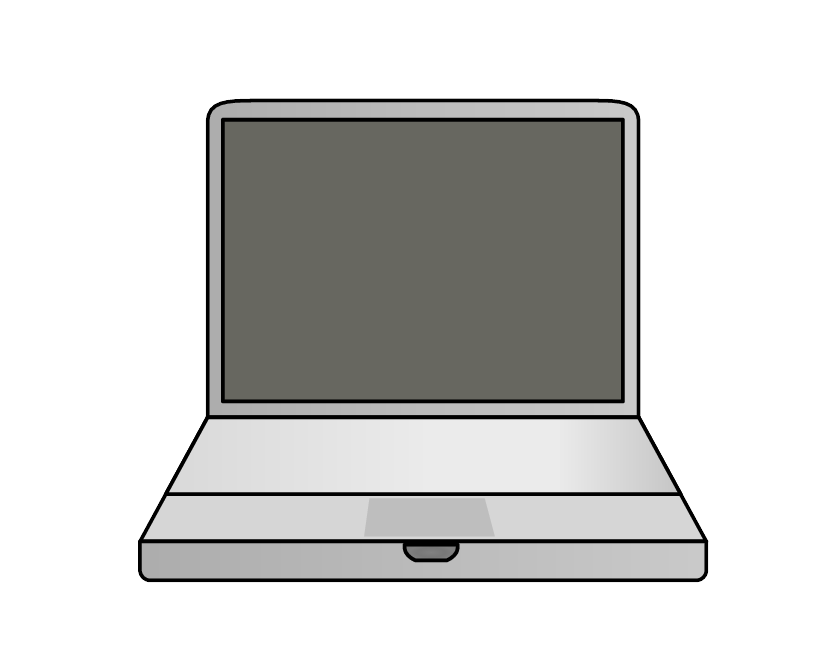
\includegraphics[width=.10\textwidth]{laptop.png}};

\node [block] (caster1) at (3,-8) {Caster 1};

\node[cloud] (ppp) at (2,0) {PPP em Tempo Real};
 
%\node [block] (relogio) at (10,-8) {Software Solução Relógios};

\node [block] (caster2) at (12,-2) {Caster 2};
\node[inner sep=0pt] (rec) at (10,-5.5) [label=below:Receptor Usuário] {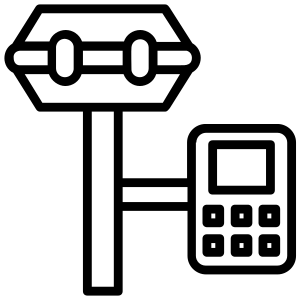
\includegraphics[width=.065\textwidth]{receiver.png}};



\draw[->,thick,shorten >=5pt] (rec1.north) -- (caster1);
\draw[->,thick,shorten >=3pt] (rec2.north) -- (caster1);
\draw[->,thick,shorten >=3pt] (recponto.north) -- (caster1);
\draw[->,thick,shorten >=5pt] (recn.north) -- (caster1);

\draw[->,thick] (caster1) -- (laptop)
    node[midway,fill=white] {Dados GNSS e Órbitas transmitidas};
    
%\draw[->,thick] (relogio) -- (laptop)    node[midway,fill=white] {Envio ao usuário};
    
\draw[->,thick] (caster2) -- (laptop) node[midway,fill=white] {Correção Órbitas/Relógios};
\draw[->,thick] (rec) -- (laptop) node[midway,fill=white] {Porta Serial};

\draw[<->,thick,shorten >=3pt] (laptop) -- (ppp) node[midway,fill=white] {Solução \textit{float} ambiguidades};;

\end{tikzpicture}}
% ---
\caption{Esquema RTPPP.}
\end{figure}


\noindent

O RTPPP se utiliza do mesmo método do PPP entretanto requer a disponibilidade em tempo real das órbitas precisas e das correções ou erros dos relógios dos satélites (não sincronização do relógio do satélite com o sistema de tempo GNSS) \citep{marques2012ppp}. Essa necessidade é devido ao fato do RTPPP proporcionar o posicionamento em tempo real. 

O RTPPP se utiliza da solução de ambiguidades pelo método ''\textit{float}'' e pode ser realizado com um receptor GNSS de dupla frequência conectado via porta serial com um computador. Esse computador deve possuir acesso a internet pois receberá dados de dois \textit{Caster}. O \textit{Caster} 1 envia para o usuário dados GNSS de outros receptores além das órbitas transmitidas dos satélites. O \textit{Caster} 2 envia ao usuário as informações de órbita e relógio do satélite. Nessas informações estão contidas a solução dos relógios dos satélites que atenua os erros dos relógios dos satélites. É possível então, em posse dos dados recebidos pelos \textit{Caster} 1 e 2 e das observáveis GNSS obtidas no receptor GNSS em questão, processar os dados e realizar o PPP em tempo real.



\newpage
\section{Introdução ao método PPP-RTK}
\noindent

O método PPP-RTK é um complemento ao PPP onde a precisão e acurácia são melhores. De acordo com \cite{wubbena2005ppp}, as limitações do método PPP podem ser superadas utilizando uma rede RTK, como as redes RTK podem obter todos os erros GNNS em tempo real o usuário pode resolver as ambiguidades e obter um nível de acurácia superior ao método PPP.

O conceito de PPP aliado a solução de ambiguidades é a síntese do PPP-RTK. A seguir encontra-se uma tabela que explicita as diferenças entre o PPP e o PPP-RTK:

\begin{table}[H]
\begin{center}
\begin{tabular}{c|c|c|}
\cline{2-3}
                                                      & \textbf{\textit{PPP}}            & \textbf{\textit{PPP-RTK}}                 \\ \hline
\multicolumn{1}{|c|}{\textbf{Tamanho da rede}}        & global                  & local/regional/	global           \\ \hline
                                                      & \multicolumn{2}{c|}{\textit{Primary state information}}    \\ \hline
\multicolumn{1}{|c|}{\textbf{Órbitas dos satélites}}  & fornecido               & fornecido                        \\ \hline
\multicolumn{1}{|c|}{\textbf{Relógios dos satélites}} & fornecido               & fornecido                        \\ \hline
\multicolumn{1}{|c|}{\textbf{Ionosfera}}              & corrigido               & fornecido                        \\ \hline
\multicolumn{1}{|c|}{\textbf{Troposfera}}             & estimado                & fornecido                        \\ \hline
\multicolumn{1}{|c|}{\textbf{Relógio do receptor}}    & estimado                & estimado                         \\ \hline
                                                      & \multicolumn{2}{c|}{\textit{Ambiguidade da fase e sinal}} \\ \hline
\multicolumn{1}{|c|}{\textbf{L1/ L2 / L0}}            & -/ - / +                & +/ + / +                         \\ \hline
\multicolumn{1}{|c|}{\textbf{Tempo de integração}}    & 30... 1800 s            & 10... 50 s                       \\ \hline
                                                      & \multicolumn{2}{c|}{\textit{Acurácia}}                     \\ \hline
\multicolumn{1}{|c|}{\textbf{3D estático}}            & $\sim$5 cm              & 1... 3 cm                        \\ \hline
\multicolumn{1}{|c|}{\textbf{RTK 3D}}                 & 15... 20 cm             & 1... 3 cm                        \\ \hline
\end{tabular}
\end{center}
\caption{Diferenças entre PPP e PPP-RTK. Adaptado de \cite{wubbena2005ppp}.}
\label{tableref}
\end{table}

Conceitualmente, o PPP-RTK é bastante similar ao método RTPPP, com a diferença que se utiliza de uma solução de ambiguidades \textit{fixa} o invés de \textit{float}. Nesse método portando o \textit{Caster} 2 proporciona uma solução de ambiguidades do tipo \textit{fixa}, mais precisa que a solução \textit{float}. A seguir um esquema que explicita o método PPP-RTK:


\begin{figure}[H]
\centering
% ---
% Taken from https://cremeronline.com/LaTeX/minimaltikz.pdf
\tikzstyle{block} = [rectangle, draw, fill=white, text width=6em, text centered, rounded corners, node distance=2cm, minimum height=2em]
\tikzstyle{cloud} = [draw, ellipse,fill=white, node distance=2cm, minimum height=2em]
\fbox{
\begin{tikzpicture}
%\node[inner sep=0pt] (sat) at (0,0) {
\includegraphics[width=.15\textwidth]{satelite.png}};
    
\node[inner sep=0pt] (rec1) at (0,-10) [label=below:Receptor 1] {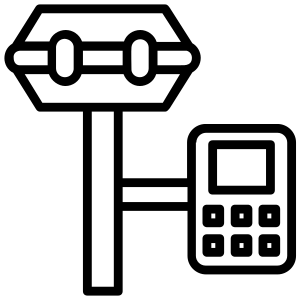
\includegraphics[width=.05\textwidth]{receiver.png}};
\node[inner sep=0pt] (rec2) at (2.5,-10) [label=below:Receptor 2] {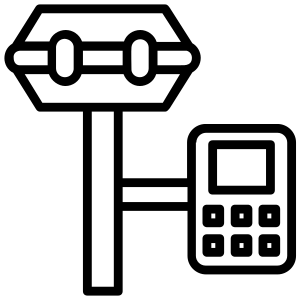
\includegraphics[width=.05\textwidth]{receiver.png}};
\node (recponto) at (5,-10) {...};
\node[inner sep=0pt] (recn) at (7.5,-10) [label=below:Receptor n] {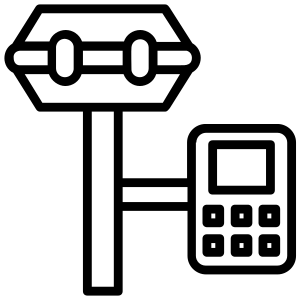
\includegraphics[width=.05\textwidth]{receiver.png}};


\node[inner sep=0pt] (laptop) at (5,-5) [label=left:Software BNC] {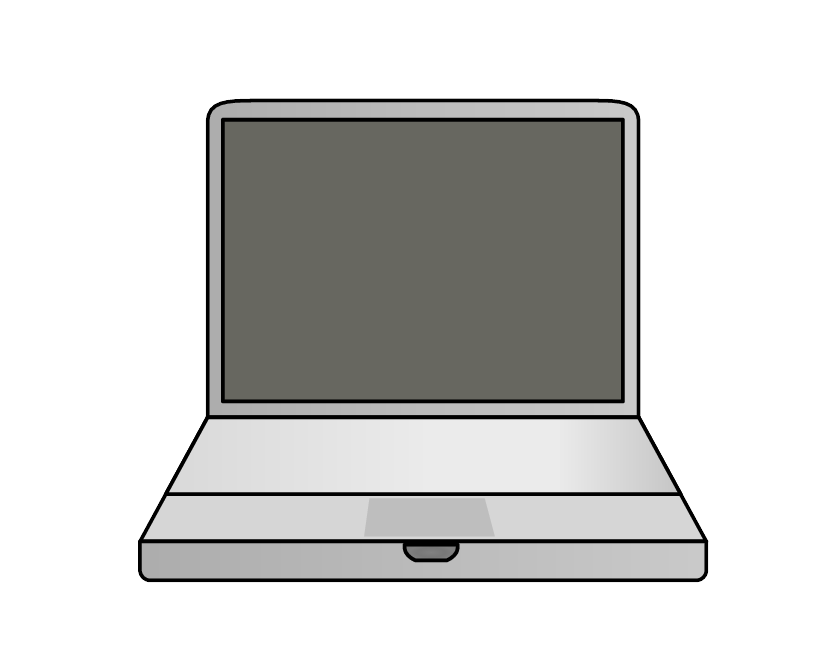
\includegraphics[width=.10\textwidth]{laptop.png}};

\node [block] (caster1) at (3,-8) {Caster 1};

\node[cloud] (ppp) at (2,0) {PPP em Tempo Real};
 
%\node [block] (relogio) at (10,-8) {Software Solução Relógios};

\node [block] (caster2) at (12,-2) {Caster 2};
\node[inner sep=0pt] (rec) at (10,-6) [label=below:Receptor Usuário] {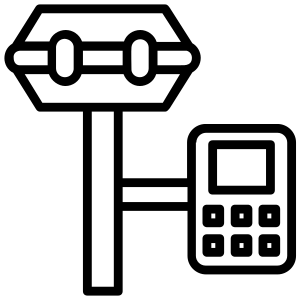
\includegraphics[width=.065\textwidth]{receiver.png}};



\draw[->,thick,shorten >=5pt] (rec1.north) -- (caster1);
\draw[->,thick,shorten >=3pt] (rec2.north) -- (caster1);
\draw[->,thick,shorten >=3pt] (recponto.north) -- (caster1);
\draw[->,thick,shorten >=5pt] (recn.north) -- (caster1);

\draw[->,thick] (caster1) -- (laptop)
    node[midway,fill=white] {Dados GNSS e Órbitas transmitidas};
    
%\draw[->,thick] (relogio) -- (laptop)    node[midway,fill=white] {Envio ao usuário};
    
\draw[->,thick] (caster2) -- (laptop) node[midway,fill=white] {Correção Órbitas/Relógios};
\draw[->,thick] (rec) -- (laptop) node[midway,fill=white] {Porta Serial};

\draw[<->,thick,shorten >=3pt] (laptop) -- (ppp) node[midway,fill=white] {Solução \textit{fixa} ambiguidades};;

\end{tikzpicture}}
% ---
\caption{Esquema PPP-RTK.}
\end{figure}


\section{RTK utilizando protocolo NTRIP}
\noindent

O georreferenciamento de áreas no Brasil é um campo de extrema importância e o desenvolvimento de novas tecnologias apoiadas na rede de telefonia móvel vem sendo aprimorado. Nesse contexto, destaca-se o uso da tecnologia RTK NTRIP, que utiliza a rede de telefonia móvel para receber correções em tempo real, através da internet \citep{LENZ2004}.

O método RTK NTRIP - \textit{Networked Transport of RTCM} via \textit{Internet Protocol} - possibilita o usuário, por meio da internet, receber as correções das estações RBMC.

De acordo com \cite{LENZ2004} , esse método foi desenvolvido pela Agência Federal de Cartografia e Geodésia da Alemanha, juntamente com a Universidade de Dortmund e a Trimble. O principal objetivo foi utilizar a internet como uma alternativa às tecnologias existentes de correção via rádio e telefonia celular.

O sistema é composto de receptores que enviam continuamente dados no formato RCTM a um servidor denominado \textit{''Caster''} e um aplicativo denominado ''Cliente'' localizado no equipamento do interessado a receber as correções. Suas principais características são:

\begin{itemize}
    \item baseado em HTTP (Hipertext Transfer Protocol);
    \item disponibilidade de distribuir qualquer tipo de dados GNSS em fluxo;
    \item capacidade de aceitar uma grande quantidade de usuários simultaneamente;
    \item o acesso aos dados é realizado de forma segura sem a necessidade de o usuário estar em contato direto com as estações de referência;
    \item habilitado a fornecer o fluxo de dados através de qualquer rede móvel TCP/IP (\textit{Transfer Control Protocol / Internet Protocol});
    \item a largura de banda necessária para disseminar as correções GNSS é relativamente pequena. Aproximadamente 5Kb/s para RTK.
\end{itemize}


O NTRIP é basicamente composto por três componentes; o NTRIP \textit{Server}, o NTRIP \textit{Caster} e o NTRIP \textit{Client}.



\begin{figure}[!htb]
\centering
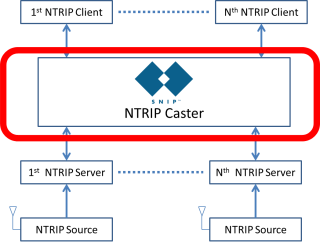
\includegraphics[scale=2.0]{img/nnnnnnn.png} %scale eh o tamanho que a figura vai ficar
\caption{Sitema NTRIP.} \citep{snip}
\label{Rotulo}
\end{figure}


O referido método é mais operacional em relação ao RTPPP e PPP-RTK pois não necessita de um computador conectador ao receptor GNSS. O receptor conectado a internet (via chip GSM) recebe informações do \textit{Caster} 1 (que faz o papel de estação base) e do \textit{Caster} 2 (que fornece informações de órbita e relógio dos satélites).

Sua vantagem em relação ao RTK convencional é ausência do link de rádio. O link de rádio que conecta a estação base a estação \textit{rover} pode ser prejudicado por obstáculos entre as estações. Contudo, pode-se ter problemas na solução de ambiguidades se a estação base conectada à internet estiver muito distante. No RTK/NTRIP o \textit{Caster} 1 faz o papel de estação base e essas informações chegam via internet. A seguir um esquema que exemplifica o RTK/NTRIP:

\begin{figure}[H]
\centering
% ---
% Taken from https://cremeronline.com/LaTeX/minimaltikz.pdf
\tikzstyle{block} = [rectangle, draw, fill=white, text width=6em, text centered, rounded corners, node distance=2cm, minimum height=2em]
\tikzstyle{cloud} = [draw, ellipse,fill=white, node distance=2cm, minimum height=2em]
\fbox{
\begin{tikzpicture}
%\node[inner sep=0pt] (sat) at (0,0) {
\includegraphics[width=.15\textwidth]{satelite.png}};
    
\node[inner sep=0pt] (rec1) at (0,-10) [label=below:Receptor 1] {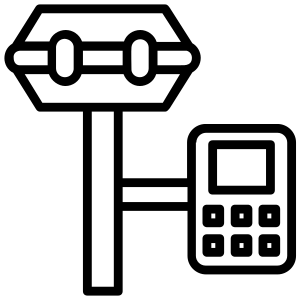
\includegraphics[width=.05\textwidth]{receiver.png}};
\node[inner sep=0pt] (rec2) at (2.5,-10) [label=below:Receptor 2] {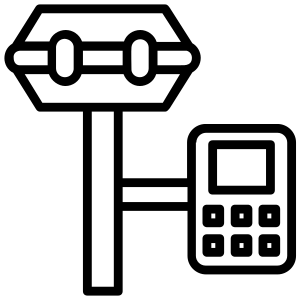
\includegraphics[width=.05\textwidth]{receiver.png}};
\node (recponto) at (5,-10) {...};
\node[inner sep=0pt] (recn) at (7.5,-10) [label=below:Receptor n] {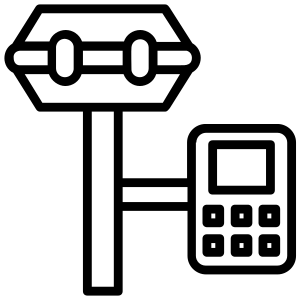
\includegraphics[width=.05\textwidth]{receiver.png}};


\node[inner sep=0pt] (laptop) at (7,-5) [label=right:Receptor usuário] {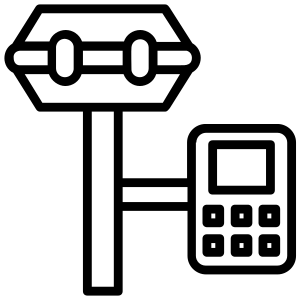
\includegraphics[width=.10\textwidth]{receiver.png}};

\node [block] (caster1) at (3,-8) {Caster 1};

\node[cloud] (ppp) at (2,-2) {RTK/NTRIP};
 
%\node [block] (relogio) at (10,-8) {Software Solução Relógios};

%\node [block] (caster2) at (12,0) {Caster 2};




\draw[->,thick,shorten >=5pt] (rec1.north) -- (caster1);
\draw[->,thick,shorten >=3pt] (rec2.north) -- (caster1);
\draw[->,thick,shorten >=3pt] (recponto.north) -- (caster1);
\draw[->,thick,shorten >=5pt] (recn.north) -- (caster1);

\draw[->,thick] (caster1) -- (laptop)
    node[midway,fill=white] {Comunicação NTRIP};
    
%\draw[->,thick] (relogio) -- (laptop)    node[midway,fill=white] {Envio ao usuário};
    
%\draw[->,thick] (caster2) -- (laptop);% node[midway,fill=white] {Solução \textit{fixa} ambiguidades};


\draw[<->,thick,shorten >=3pt] (laptop) -- (ppp) {};

\end{tikzpicture}}
% ---
\caption{Esquema RTK/NTRIP.}
\end{figure}

\section{Sistema Geodésico Local}
O Sistema Geodésico Local (SGL) é um sistema que é composto por três eixos (e,n,u) que são mutuamente ortogonais. O eixo ''n'' aponta em direção ao norte geodésico, o eixo ''e'' aponta para a direção leste, sendo que os eixos ''n'' e ''e'' estão contidos no plano topocêntrico. Por fim, o eixo ''u'' coincide com a normal do elipsoide que passa pelo vértice escolhido como a origem do sistema \citep{ibge_imoveis}. A figura a seguir ilustra o SGL.

\begin{figure}[H]
\centering
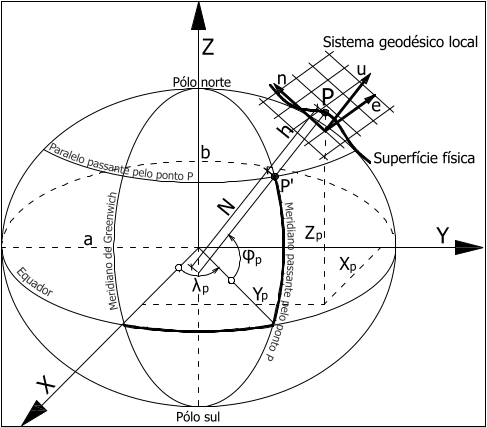
\includegraphics[scale=0.7]{img/sgl.png} %scale eh o tamanho que a figura vai ficar
\caption{Sitema Geodésico Local.} \citep{ibge_imoveis}
\label{Rotulo}
\end{figure}

O seguinte modelo matemático é utilizado para calcular as coordenadas geodésicas locais:

\small
\begin{equation}
\label{sgl_mod_mat}
\begin{bmatrix}
e\\
n\\
u
\end{bmatrix}
=
\begin{bmatrix}
1 & 0 & 0\\
0 & \sin{\varphi_0} & \cos{\varphi_0}\\
0 & -\cos{\varphi_0} & \sin{\varphi_0}
\end{bmatrix}
\begin{bmatrix}
-\sin{\lambda_0} & \cos{\lambda_0}\\
-\cos{\lambda_0} & -\sin{\lambda_0} & 0\\
0 & 0 & 1
\end{bmatrix}
\begin{bmatrix}
X-X_0\\
Y-Y_0\\
Z-Z_0
\end{bmatrix}
\end{equation}
\normalsize

Em que:
\begin{itemize}
    \item \textit{e, n, u} - são as coordenadas cartesianas locais do vértice de interesse;
    \item \textit{X, Y, Z} - são as coordenadas cartesianas geocêntricas do vértice de interesse;
    \item $\varphi_0$, $\lambda_0$ - são a latitude e a longitude adotadas como origem do sistema;
    \item $X_0$, $Y_0$, $Z_0$ - são as coordenadas cartesianas geocêntricas adotadas como origem do sistema.
\end{itemize}
\chapter{Materiais e Métodos}


\section{Equipamentos e Softwares}
\label{materiais}

A seguir, serão apresentados os equipamentos e recursos utilizados para o processamento em tempo real e o pós-processamento.

\begin{itemize}

\item Processamento: As conexões aos Casters são feitas via software, o qual realiza o processamento dos dados em tempo real. Será utilizada a plataforma de software livre” BKG Ntrip Client (BNC) 2.12.9”. Já para o pós-processamento, ''Topcon Tools 8.2.3.19157'' e ''Magnet Tools''.    

\item Software BKG Ntrip Client (BNC): Recupera, decodifica, converte e processa fluxos de dados GNSS em tempo real (BNC, 013). Além da principal funcionalidade de processamento em tempo real, ainda possui algumas funcionalidades de pós-processamento. Tal ferramenta foi desenvolvida no âmbito do IAG para o sistema EUREF e para o IGS. O BKG Ntrip Client (BNC) foi escrito uma licensa aberta, a GNU General Public License (GPL), desta forma seu código é aberto e está disponivel em http://software.rtcm-ntrip.org/svn/trunk/BNC.
        
        Abaixo estão alguns dos propósitos do BNC \citep{bnc}:
        \begin{itemize}
            \item recuperar fluxos de dados GNSS em tempo real disponíveis através do protocolo de transporte NTRIP;
            \item recuperar fluxos de dados GNSS em tempo real via TCP diretamente de um endereço IP sem usar o NTRIP protocolo de transporte;
            \item recuperar fluxos de dados GNSS em tempo real a partir de uma porta UDP ou serial local sem usar o NTRIP protocolo de transporte;
            \item gerar arquivos de Observação e Navegação RINEX de alta taxa para suportar aplicações GNSS pós-processadas quase em tempo real;
        \end{itemize}

\item Computador: Para a utilização dos softwares de processamento em tempo real e pós processamento o o computador ''Intel(R) Core (TM) i5-7200U CPU @ 2.50GHz'' será utilizado;

\item Receptor GNSS: para as medições em campo será utilizado o receptor ”Topcon GR5”, da Seção de Engenharia Cartográfica do Instituto Militar de Engenharia. Cabe ressaltar que esse possui comunicação via celular SIM Card, GSM/CDMA ou HSPA interno no receptor e suporte à tecnologia NTRIP, requisito para a realização do RTK/NTRIP.

\item Coletor de dados: Tablet Topcon FC-5000. Esse equipamento possibilita conexão direta com o GR-5, com um sistema operacional Windows 10, é um computador de bordo no campo de operações.
         
\end{itemize}


\section{Métodos}
\noindent

Os métodos escolhidos para esse projeto visam demonstrar a viabilidade da aplicação das técnicas de posicionamento utilizando GNSS em tempo real. Ademais, busca-se mostrar as etapas e ferramentas necessárias para cada método de posicionamento, visto que em projetos e aplicações de engenharia, a implementação inicial de métodos novos e pouco consolidados é uma etapa adicional em relação a métodos já estabelecidos.

Neste projeto serão obtidas as acurácias esperadas do RTK (RTPPP e RTK/NTRIP) e do PPP-RTK, bem como as etapas práticas necessárias para a sua realização, no sentido de fornecer as informações necessárias para a escolha de cada método adequado para cada situação específica.

\subsection{RTPPP com estação da RBMC}

\begin{itemize}
    \item Primeiramente, por intermédio do BNC, a avaliação do RTPPP será feita utilizando uma estação estática da Rede Brasileira de Monitoramento Contínuo, RBMC:
    \begin{itemize}
        \item Estação escolhida: Porto Alegre (POAL) – Estação pertencente à Rede de Densificação do IGS e à Rede de Referência do SIRGAS;
        \item Coordenadas em SIRGAS 2000 na época 2019.48:
        \begin{itemize}
            \item X: 3467519.4343 m;  Y: -4300378.65881 m; Z: -3177517.52227 m \citep{sirgascon}.
        \end{itemize}
        \item A escolha de uma estação estática para a primeira coleta e processamento de dados é fundamental para o entendimento prático do método:
            \begin{itemize}
            \item Coordenadas de alta precisão e confiabilidade para trabalhos futuros;
            \item Posição da estação simulando a ideal, elevada e com o mínimo de obstruções a fim de coletar o máximo de sinais;
            \item Antena \textit{choke ring} (TRM59800.00) a qual é a ideal para atenuar os efeitos de multicaminho.
            \end{itemize}

        \item O software coletará em tempo real, com um intervalo de 01 segundo durante o período de 24h os dados brutos (em formato RINEX) da estação POAL através da conexão:
        \begin{itemize}
            \item www.igs-ip.net, porta 2102, \textit{mountpoint} POAL00BRA0.
        \end{itemize}
        
        \item Simultaneamente com dados da estação POAL, o software coletará os dados das órbitas transmitidas e relógios dos satélites, bem como a solução dos relógios dos satélites para atenuar os erros de relógio. Tais dados serão coletados a partir das seguintes conexões:
        \begin{itemize}
            \item Caster 1: products.igs-ip.net, porta 2101, \textit{mountpoint} CLK91.
            \item Caster 2: products.igs-ip.net, porta 2101, \textit{mountpoint} RTCM3EPH.
        \end{itemize}
        \item Após a coleta, ter-se-ão as informações das coordenadas cartesianas da estação POAL para cada segundo, bem como as variações das coordenadas no sistema geodésico local (dE, dN, dU). Desta forma, os dados de dE, dN e dU são extraidos e constroi-se um gráfico de série temporal com esses dados.
    
    \end{itemize}
    \item Configuração do BNC para RTPPP - serão observados os seguintes detalhes:
    \begin{itemize}
        \item Indicação dos caminhos para armazenamento do \textit{log} do RTPPP e dos RINEX. Na aba ''PPP(1)'' seleção de ''\textit{Real-time streams}'' na opção de ''\textit{data-source}''. ''\textit{CLK91}'' em ''\textit{corrections stream}''. Indicação do caminho para o arquivo (igs14.atx) que contém as especificações de antenas disponível em \cite{ngsatx}.
        \item No arquivo com as coordenadas da estação utilizada deve-se especificar o modelo de antena do receptor.
    \end{itemize}
\end{itemize}

\subsection{RTK com GR-5}


Com o intuito de realizar as configurações iniciais do receptor, bem como verificar o correto armazenamento das observáveis obtidas pelo receptor. serão realizados um Posicionamento por Ponto e um RTK utilizando o marco do IBGE ''91780'', localizado no terraço do quinto andar do prédio frontal do IME.

\begin{itemize}
    \item Ambientação com o equipamento: Como o GR-5 é recém-chegado na Seção de Engenharia Cartográfica, é necessário realizar as configurações do aparelho, por exemplo: 
    \begin{itemize}
        \item Atualização de Firmware;
        \item Configuração de hemisfério (procedência estadunidense, ou seja, alterar a opção de hemisfério norte para sul, afim de rastrear os satélites corretamente);
        \item Fuso horário;
        \item Sistema de Referência;
        \item Comunicação via link de rádio;
        \item Configuração da controladora.
    \end{itemize}
    \item Testes Iniciais: Com o apoio da equipe de topografia da sessão, foram realizadas verificações do funcionamento básico do aparelho: sistema de coordenadas, bateria, conexão bluetooth à controladora e via porta serial com notebook;
    
    \item Levantamentos:
    
    Posicionamento por Ponto Estático e RTK: A fim de verificar a gravação de dados pela Base e a confirmação da coerente medição de pontos, optou-se por realizar um PP Estático. Arquivos RINEX de observação foram gerados para análise;

    
\end{itemize}


\section{Comparação entre os métodos}


Ao coletar dados por meio dos receptores e dos Casters e registrá-los em formato RINEX, pode-se realizar a avaliação da acurácia. Pós-processando esses dados, temos uma solução confiável para realizar as comparações. 


\section{Especificações técnicas}

Com o intuito de facilitar e disseminar a utilização dos métodos aqui estudados o presente trabalho visa fornecer especificações técnicas que tratem a respeito da realização dos métodos de RTPPP, PPP-RTK e RTK/NTRIP. Tal especificação deverá conter o seguinte:
\begin{itemize}
    \item especificação dos equipamentos utilizados em cada um dos métodos;
    \item esquema das medições;
    \item especificação dos softwares utilizados;
    \item etapas necessárias para a realização de cada método;
    \item etapas necessárias para o processamento em tempo real e pós-processamento dos dados; e
    \item acurácia esperada para cada método.
\end{itemize}

\section{Cronograma}
\noindent

Segue na Figura \ref{fig:cronograma} o cronograma com as atividades previstas para o desenvolvimento do Projeto. Considera-se como período útil à realização do projeto de 12 de fevereiro de 2019 a 17 de outubro de 2019.

\begin{figure}[H]
	\centering  
	\caption{Cronograma de Projeto}
	\label{fig:cronograma}
    
	\begin{ganttchart}[
    y unit title=0.4cm,
    y unit chart=0.5cm,
    vgrid,
    time slot format=isodate-yearmonth,
    compress calendar,
    title/.append style={draw=none, fill=verylightgray},
    title label font=\sffamily\bfseries\color{black},
    title label node/.append style={below=-1.6ex},
    title left shift=.05,
    title right shift=-.05,
    title height=1,
    bar/.append style={draw=none, fill=gray},
    bar height=.6,
    bar label font=\normalsize\color{black!50},
    group right shift=0,
    group top shift=.6,
    group height=.3,
    group peaks height=.2,
    bar incomplete/.append style={fill=silver},
    progress label text= %completo%    }%
   ]{2019-01}{2019-12}
   
    \gantttitlecalendar{year}\\
    \ganttgroup{Definição de Projeto}{2019-02}{2019-05} \\
        \ganttbar[progress=100, name=T1A]{Validação do Tema}{2019-02}{2019-05} \\
        \ganttbar[progress=100]{Definição da Metodologia}{2019-03}{2019-05} \\
    
    \ganttgroup{Revisão Bibliográfica}{2019-02}{2019-07} \\
        \ganttbar[progress=100, name=T2A]{Revisão sobre os métodos}{2019-02}{2019-07} \\
    
    \ganttgroup{Medições}{2019-07}{2019-09} \\
        \ganttbar[progress=100, name=T2A]{Medições em campo}{2019-07}{2019-09} \\
        
    \ganttgroup{Processamento dos dados}{2019-07}{2019-09} \\
        \ganttbar[progress=100]{Processamento}{2019-07}{2019-09}\\
        
    \ganttset{link/.style={green}}
    \ganttgroup{Análises de Resultados}{2019-08}{2019-10} \\
        \ganttbar[progress=100]{Comparações}{2019-08}{2019-10}\\
        
    \ganttgroup{Produção Textual}{2019-03}{2019-11} \\
        \ganttbar[progress=100]{Relatório I}{2019-03}{2019-05}\\
        \ganttbar[progress=100]{Relatório II}{2019-06}{2019-07}\\
        \ganttbar[progress=100]{Relatório III}{2019-08}{2019-10}\\
        %\ganttbar[progress=0]{Artigo*}{2019-10}{2019-10.5}\\
\end{ganttchart}
\end{figure}






São descritos a seguir de forma breve as atividades pretendidas para cada um dos itens descritos no cronograma apresentado:

\begin{enumerate}
    \item Definição de Projeto 
        \begin{enumerate}
            \item Validação do Tema: a etapa visa a validação da proposta do projeto, com a definição dos objetivos, verificação de trabalhos que tratem a respeito do assunto e a verificação e explanação da necessidade de realização do projeto.
            
            \item Definição da metodologia: definição da metodologia a ser seguida para que se alcancem os objetivos propostos.
        \end{enumerate}

    \item Revisão Bibliográfica
        \begin{enumerate}
            \item Revisão sobre os métodos: a etapa visa realizar a revisão bibliográfica sobre os métodos utilizados no presente trabalho assim como outros métodos relacionados que servirão de base para a confecção do relatório.
        \end{enumerate}

    \item Medições
        \begin{enumerate}
            \item Medições em campo: realização das medições com aparelho GNSS (modelo ''GR-5'') na Praça General Tibúrcio (Rio de Janeiro - RJ) e também com computador conectado a internet.
        \end{enumerate}
    
    \item Processamento
        \begin{enumerate}
            \item Processamento dos dados: realização do processamento em laboratório dos dados coletados na etapa de Medições a fim de gerar uma solução mais confiável que servirá de base para comparação e definição das acurácias alcançadas com os métodos. O processamento visa utilizar ferramentas de software livre e softwares licenciados de posse da Seção de Engenharia Cartográfica do Instituto Militar de Engenharia.
        \end{enumerate}

    \item Análise de Resultados
        \begin{enumerate} 
            \item Comparações: esta etapa visa comparar o resultados das medições em campo com o resultado das medições pós-processadas de forma que seja possível estabelecer uma precisão para as medições em campo.
        \end{enumerate}

    \item Produção Textual
        \begin{enumerate} 
            \item Relatórios: produção de relatórios parcial (I e II) e final (III).
            \item Artigo*: produção de artigo (a definir) acerca do tema desenvolvido ao longo do projeto.
        \end{enumerate}
\end{enumerate}
\chapter{Resultados}
%\noindent
O capítulo apresenta os resultados obtidos ao realizar os procedimentos especificados na metodologia. Etapas e especificações complementares são descritos com o intuito de facilitar o entendimento dos procedimentos executados.

\section{RTPPP com estação da RBMC}

Primeiramente, foi realizado um RTPPP utilizando a estação POAL da RMBC sem a especificação da antena utilizada pelo receptor. A ausência das informação da antena se deu pelo fato da versão mais atual do software utilizado (BNC 2.12) ter alterado o modo de inserção de tal informação em relação a versões anteriores (BNC 2.9). Na versão 2.12 as informações de antena devem ser inseridas juntamente com o arquivo de coordenadas.

Seguem os resultados:

\begin{figure}[H]
\centering
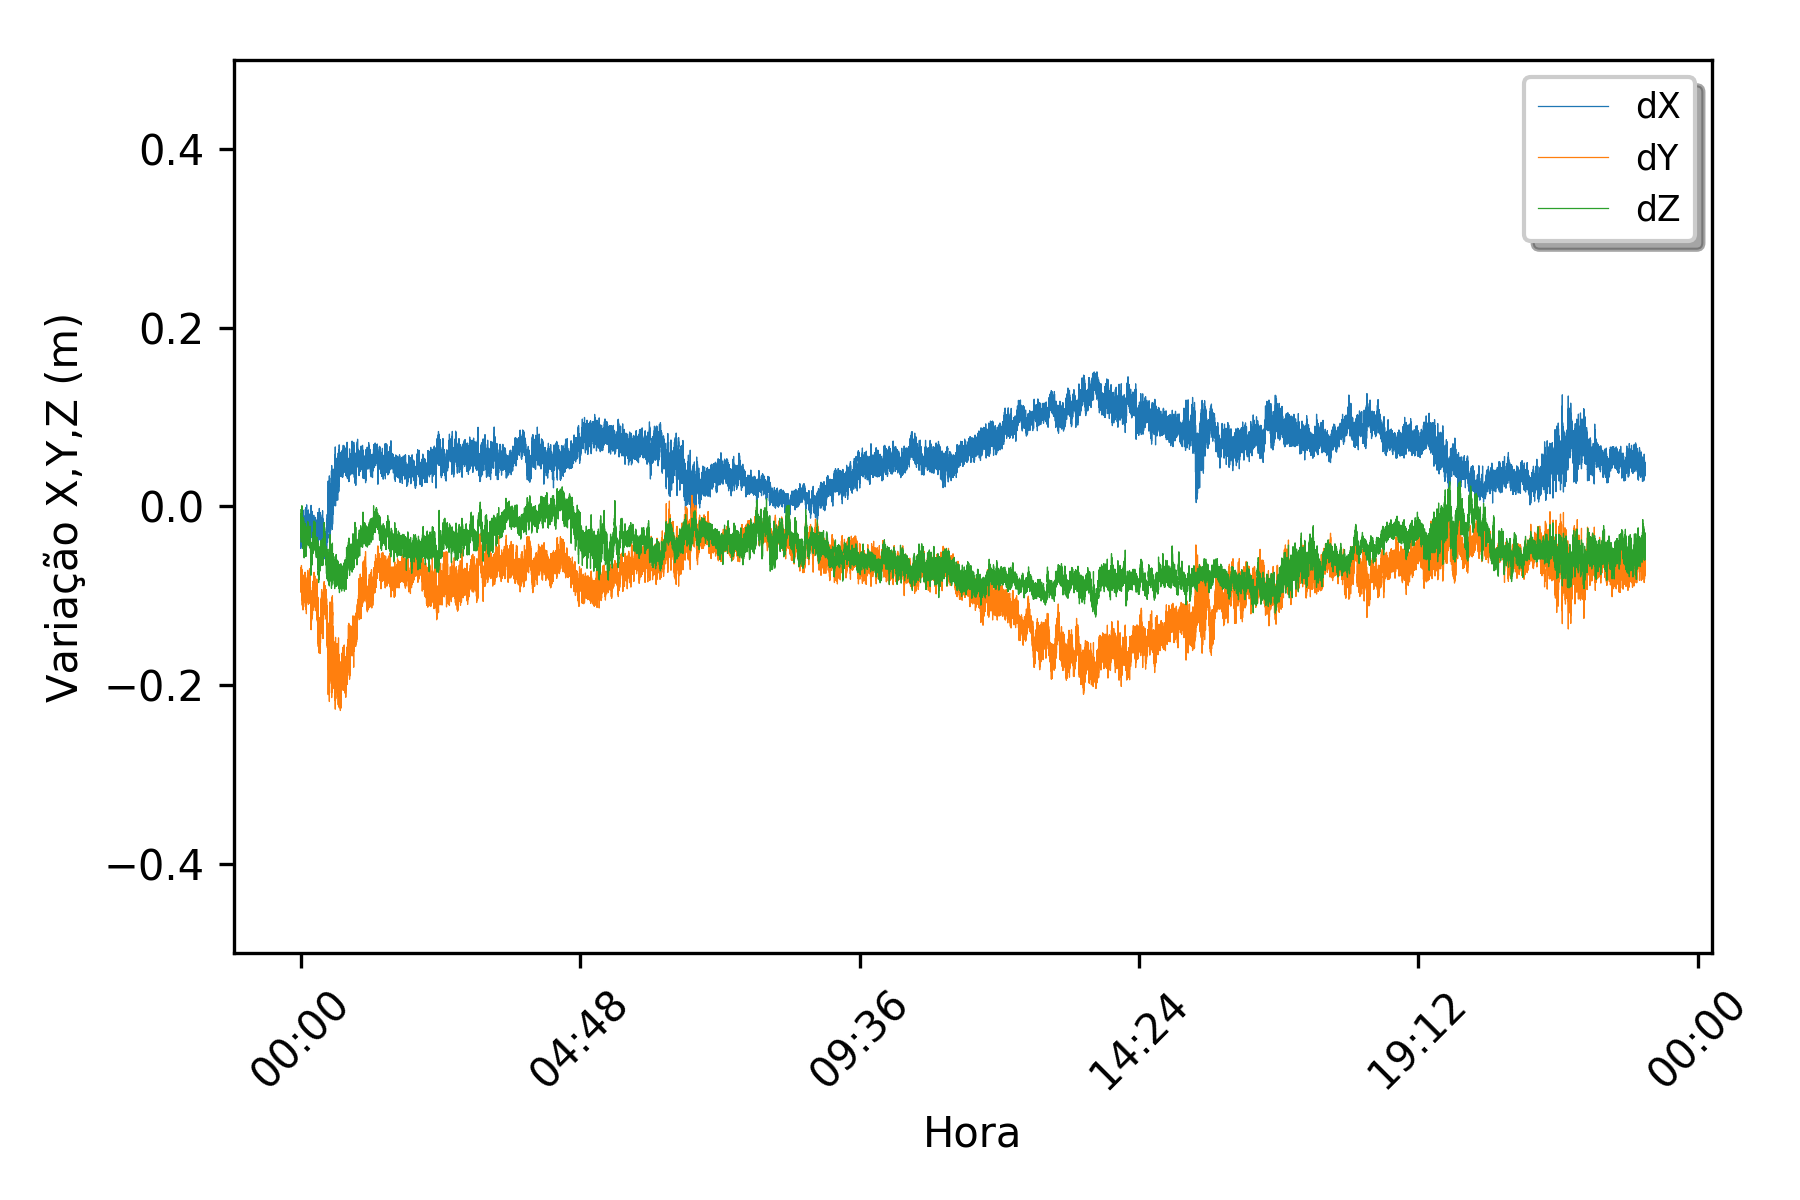
\includegraphics[scale=0.9]{data/Graphics/POAL20636/POAL20636_graphic_xyz.png}
\caption{Série temporal RTPPP - dX, dY, dZ.}
\label{rtppp1}
\end{figure}

As coordenadas utilizadas como referência para os cálculos de dX, dY e dZ para cada época foram as coordenadas obtidas em \cite{sirgascon} para a semana GPS 2065.

Pode-se observar na fig. \ref{rtppp1} que desde o início da coleta de dados o RTPPP apresentou variações relativamente pequenas nas componentes dX, dY, dZ; entretanto é possível observar uma tendência nas três componentes.

\begin{figure}[H]
\centering
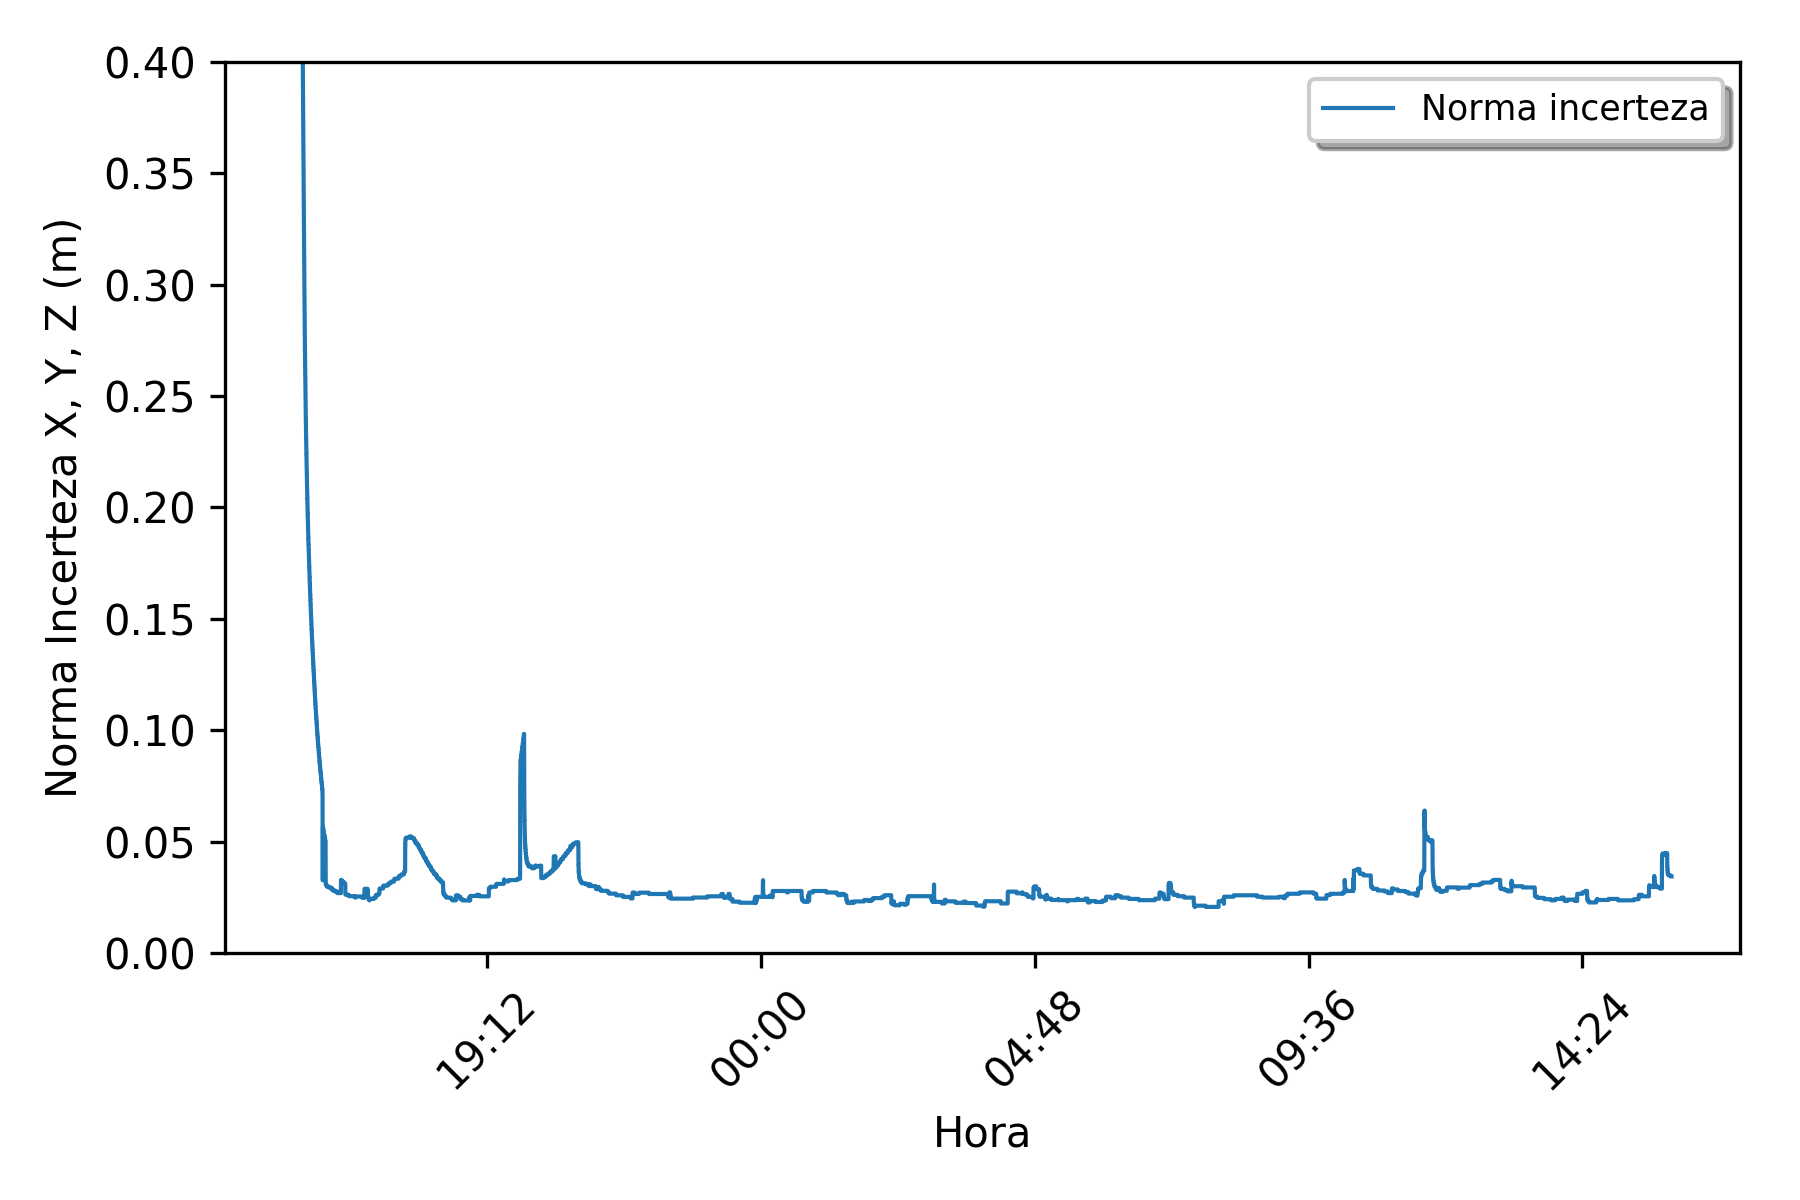
\includegraphics[scale=0.9]{data/Graphics/POAL001_ppp_wizard/POAL001_ppp_wizard_graphic_uncertainty.png}
\caption{Série temporal RTPPP - Incerteza das coordenadas X, Y, Z.}
\label{incert1}
\end{figure}

Pelo fato de estar-se realizando um PPP em tempo real, uma possibilidade para verificar a qualidade dos dados em tempo real é verificar a incerteza das coordenadas X, Y e Z que são obtidas em tempo real. A norma das incertezas das coordenadas X, Y e Z na fig. \ref{incert1} variou entre aproximadamente 5 e 14 cm.

\begin{figure}[H]
\centering
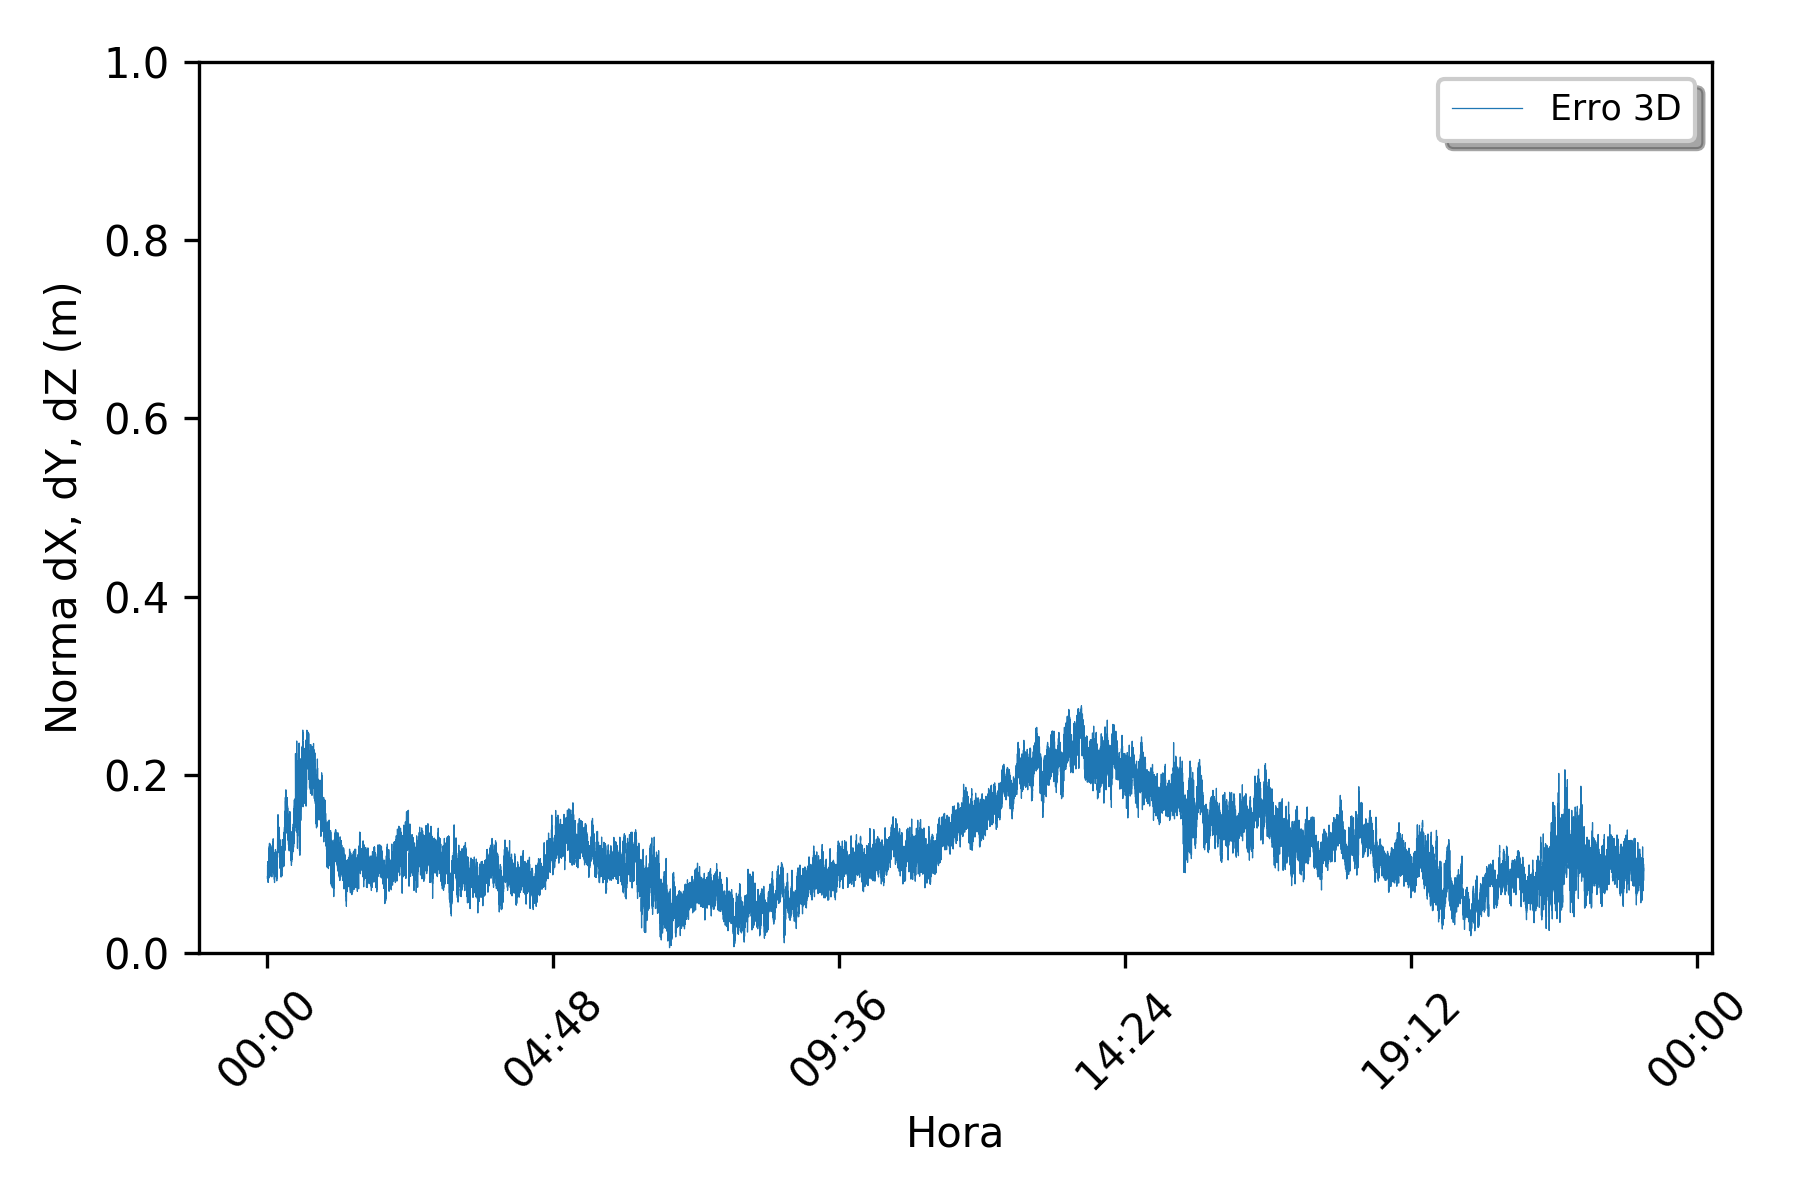
\includegraphics[scale=0.9]{data/Graphics/POAL20636/POAL20636_graphic_result.png}
\caption{Série temporal RTPPP - Resultante dX, dY, dZ.}
\label{result1}
\end{figure}

Na fig. \ref{result1} pode-se observar que a norma do vetor resultante de dE, dN e dU variou entre aproximadamente 22 cm e 37 cm. Tal variação é acima do esperado para um PPP mas provavelmente reflete as tendências causadas pela ausência de informações da antena do receptor.

Após isso, utilizando a mesma estação, realizou-se um RTPPP com a especificação da antena utilizada pelo receptor. A seguir os resultados:

\begin{figure}[H]
\centering
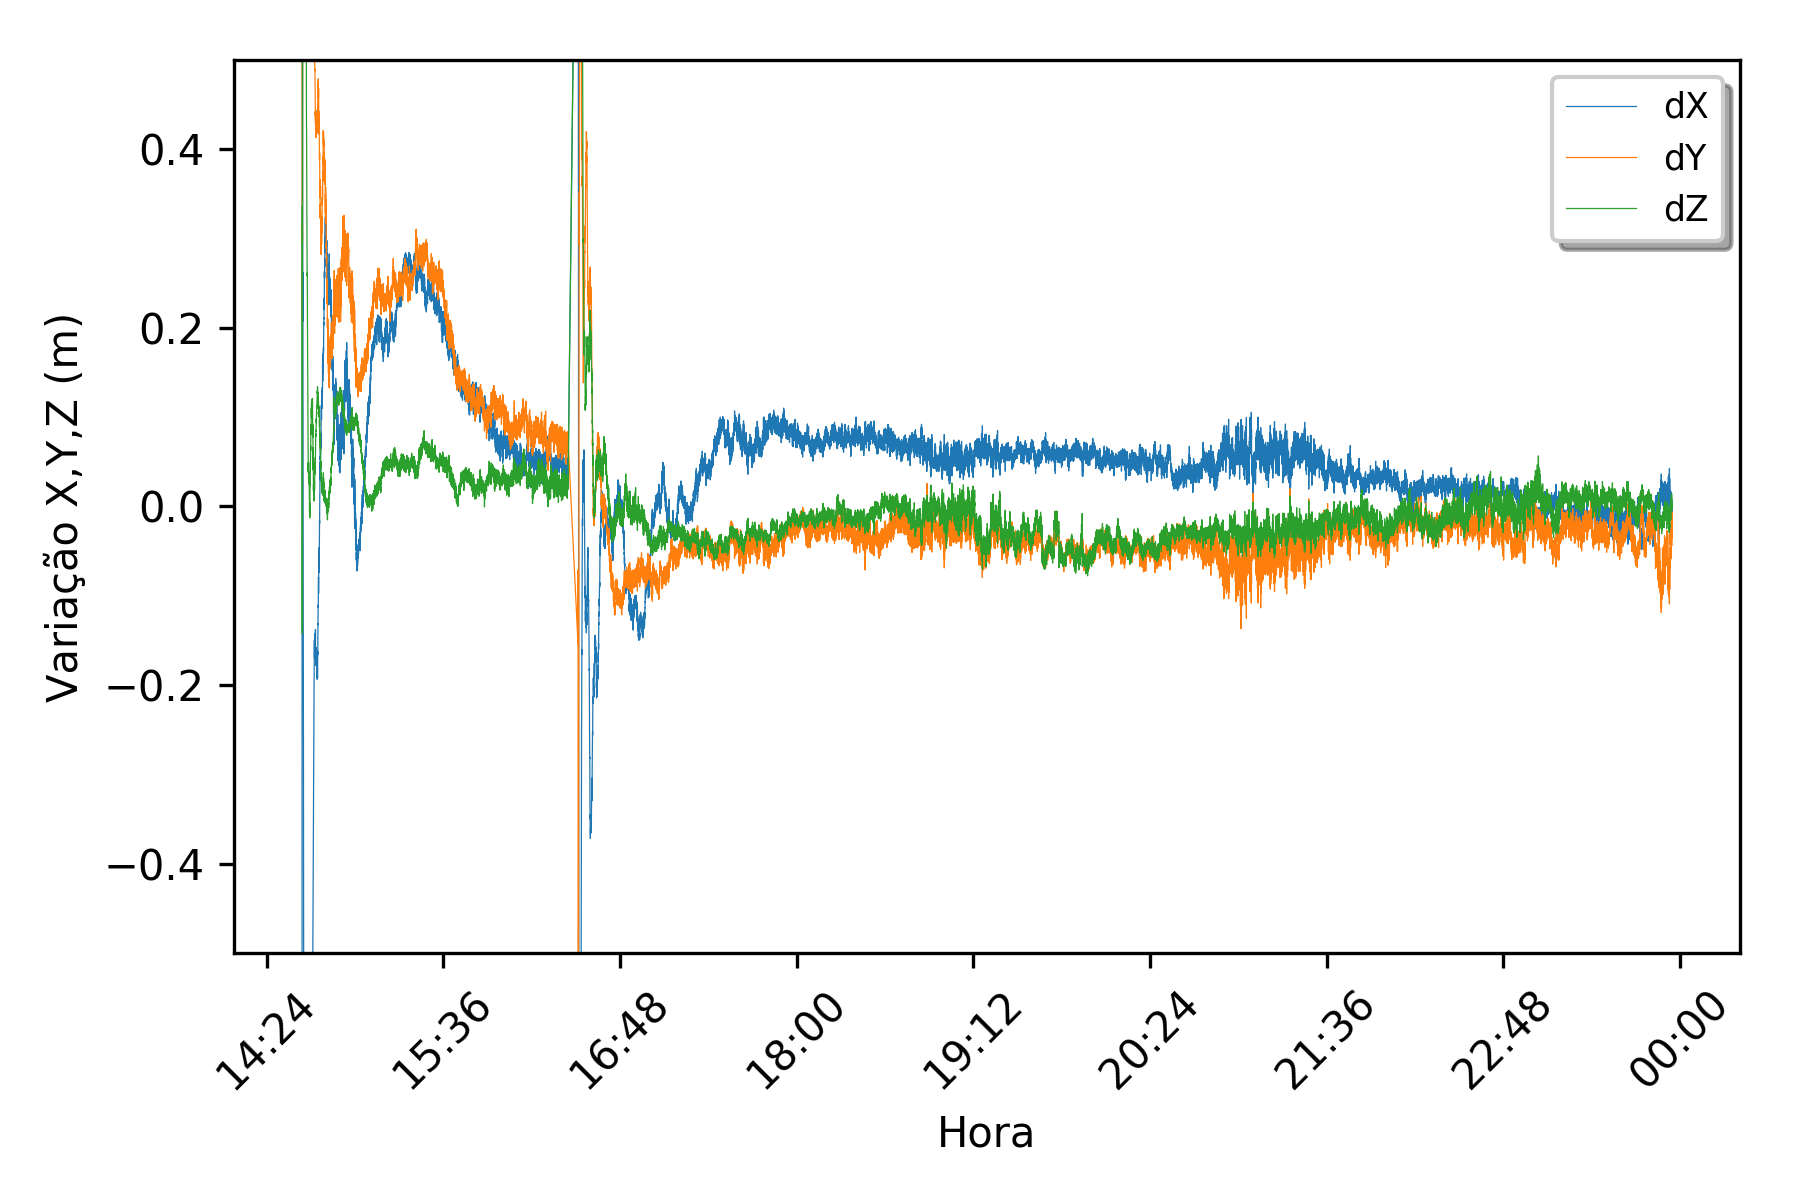
\includegraphics[scale=0.9]{data/Graphics/POAL20650/POAL20650_graphic_xyz.png}
\caption{Série temporal RTPPP - dX, dY, dZ.}
\label{rtppp2}
\end{figure}

Na fig. \ref{rtppp2} pode-se observar que o PPP convergiu para valores menores que 40 cm em aproximadamente 10 minutos. Observa-se um pico nos valores por volta de 15:50 devido a uma queda de conexão, mas com conversão para valores inferiores a 20cm em menos de 10 minutos. Nas horas finais, observa-se que os valores variam em menos de 10 cm.

\begin{figure}[H]
\centering
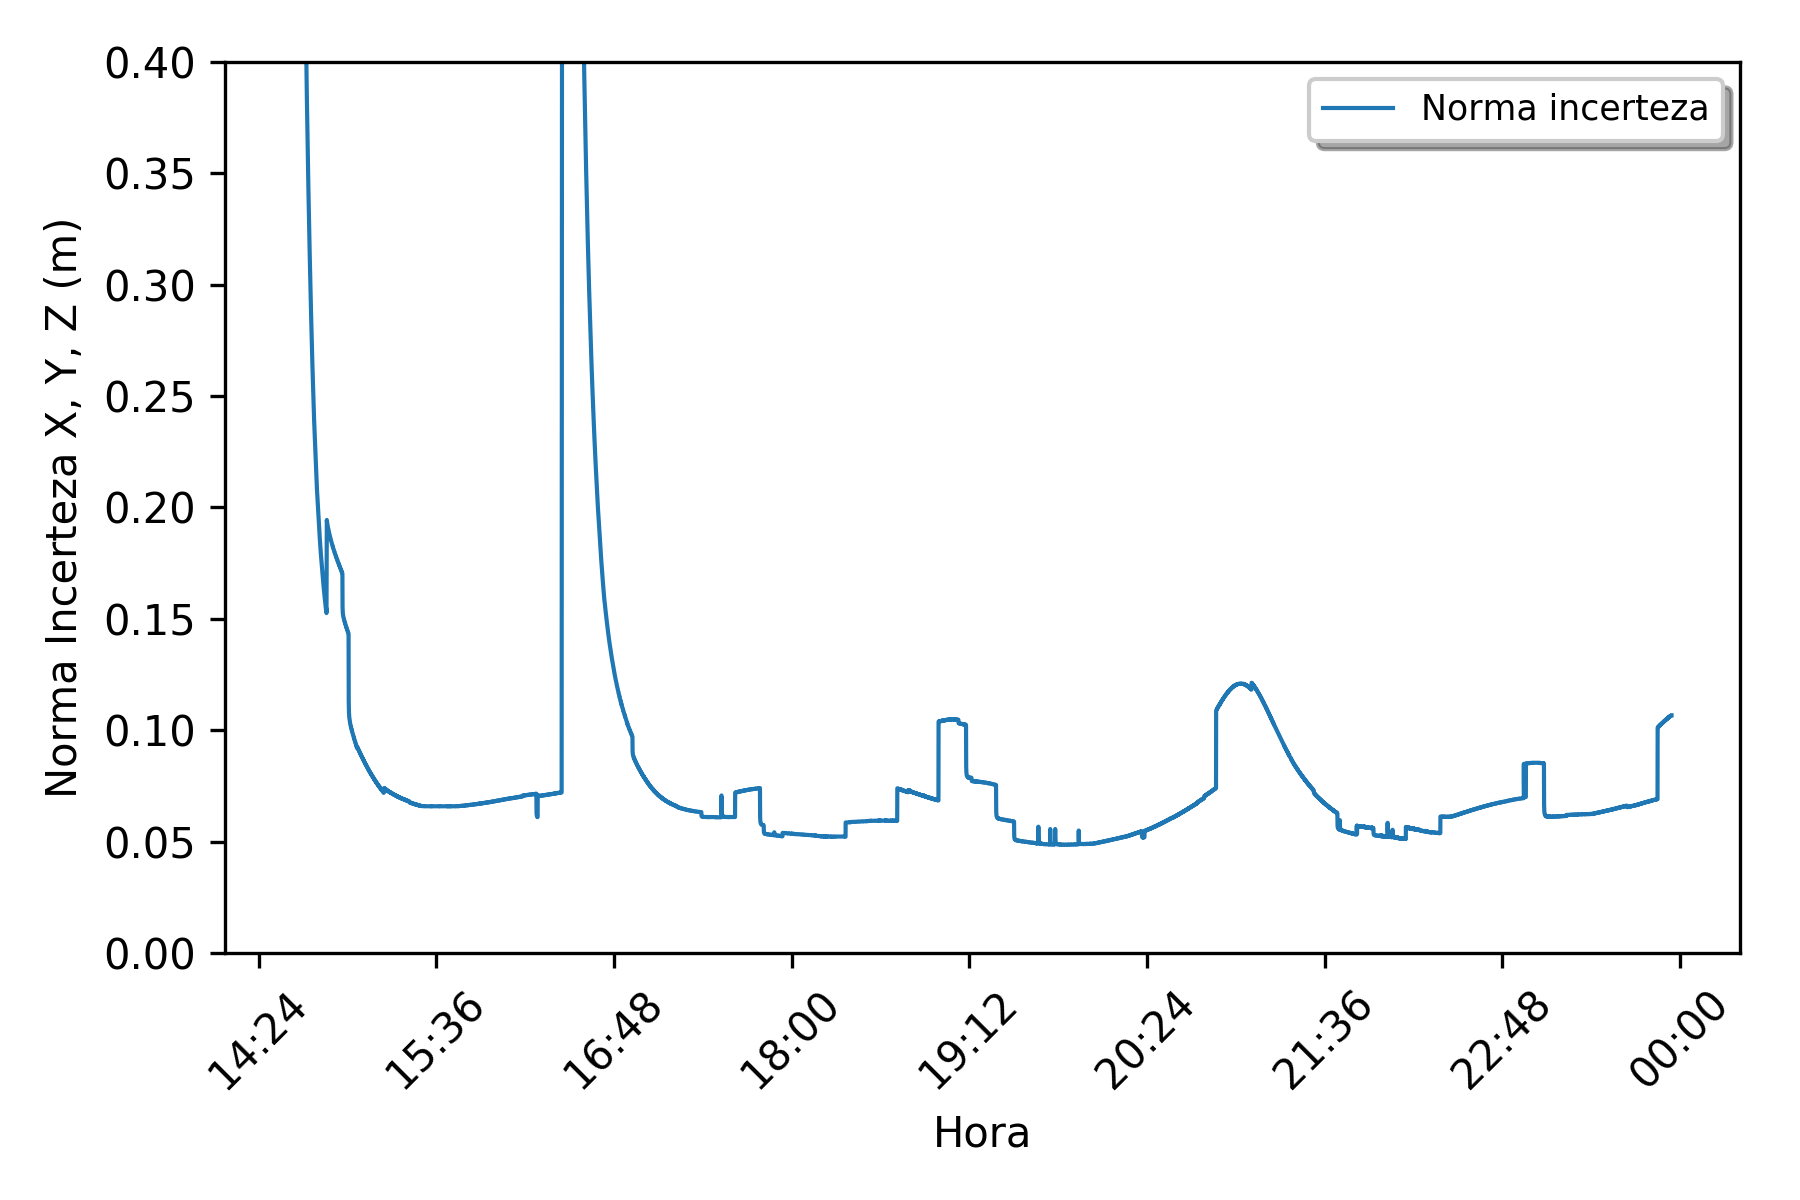
\includegraphics[scale=0.9]{data/Graphics/POAL20650/POAL20650_graphic_uncertainty.png}
\caption{Série temporal RTPPP - Incerteza das coordenadas X, Y, Z.}
\label{incert2}
\end{figure}

Na fig. \ref{incert2} observa-se que a resultante das incertezas das coordenadas X, Y e Z variou, na maior parte do tempo, entre aproximadamente 5 e 15 cm. 

\begin{figure}[H]
\centering
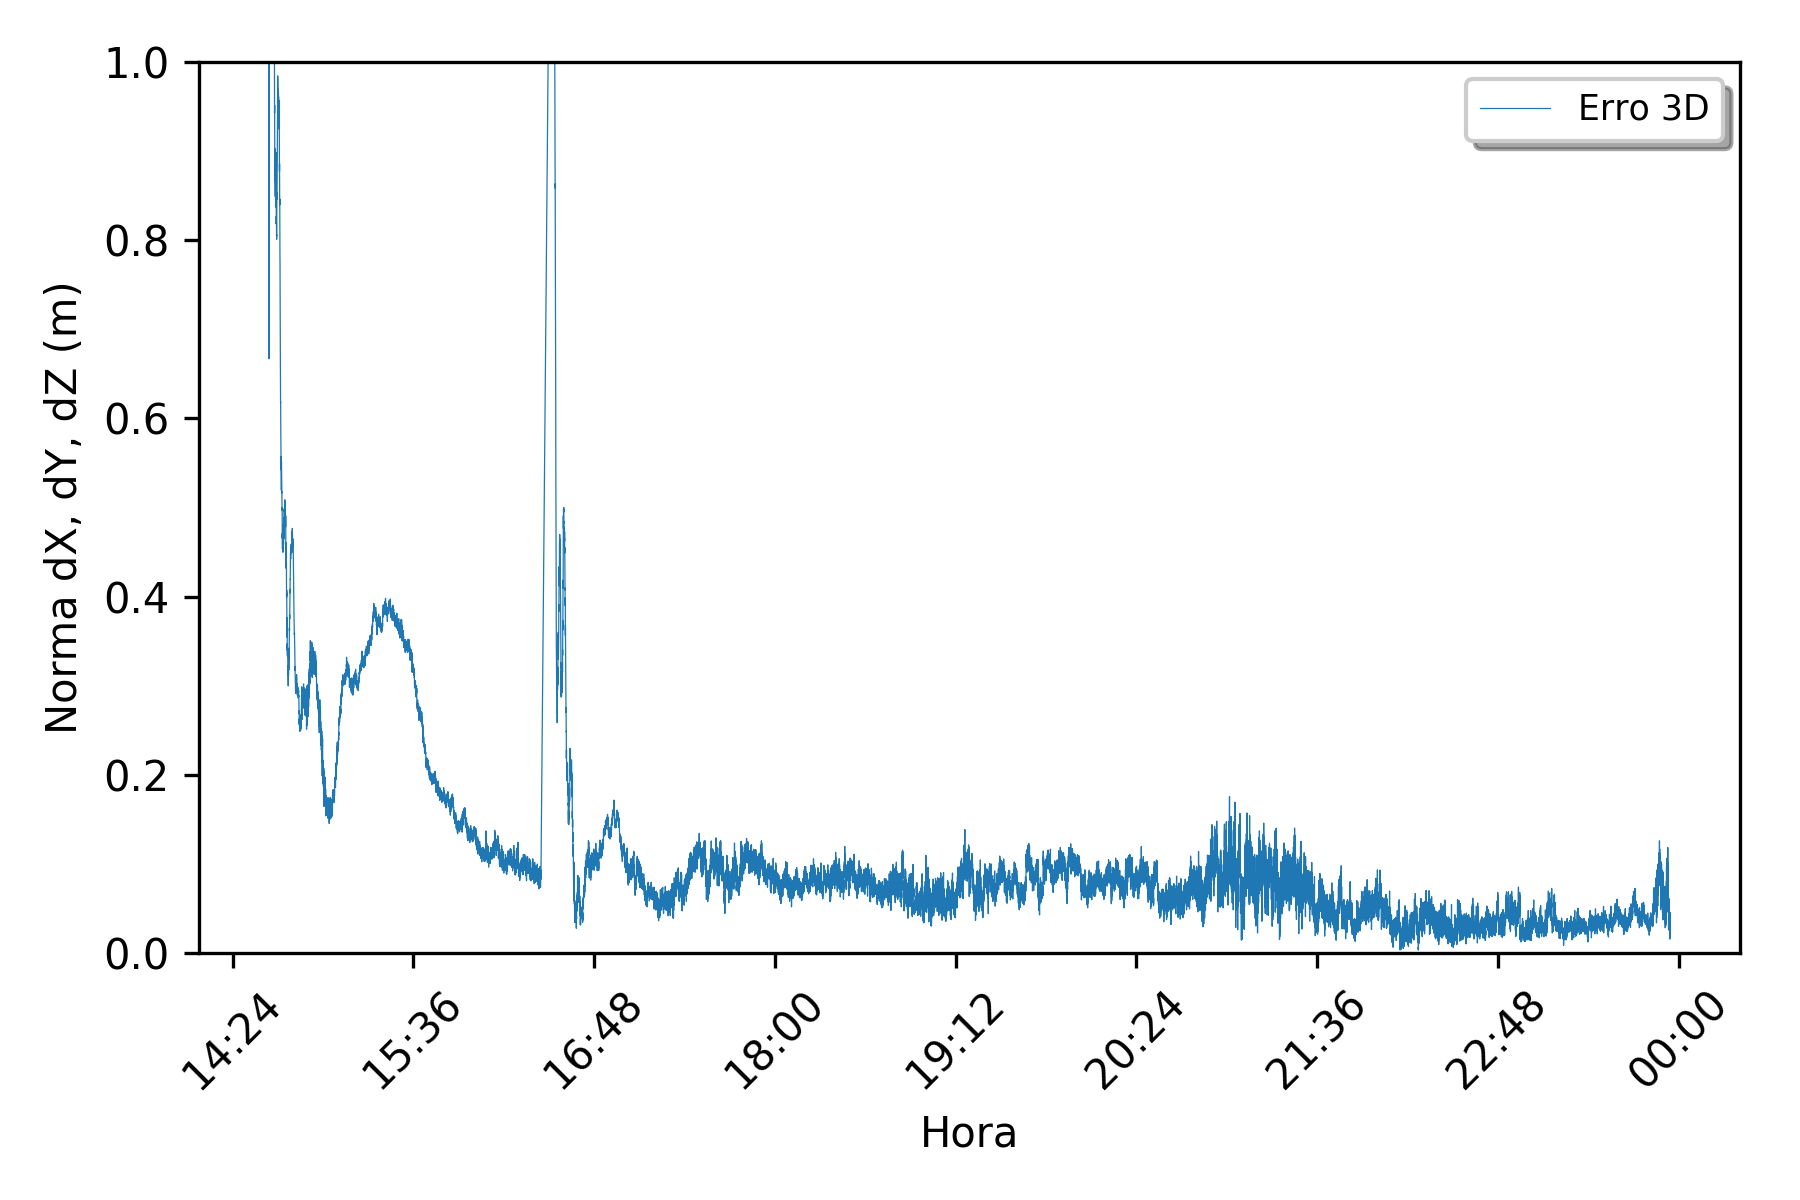
\includegraphics[scale=0.9]{data/Graphics/POAL20650/POAL20650_graphic_result.png}
\caption{Série temporal RTPPP - Norma de dX, dY, dZ.}
\label{}
\end{figure}

\section{RTPPP com GR-5}
\subsection{RTPPP em estação estática}
Com o objetivo de atender a proposta de realizar-se um RTPPP utilizando ferramentas de software livre, realizou-se em 17 de setembro de 2019 uma coleta de dados com o receptor GR-5 conectado a um notebook com o software BNC. O receptor estava no marco ''91752'' do IBGE, localizado no terraço do prédio dos fundos do IME. A conexão do receptor com o computador foi feita utilizando um cabo Serial/Porta-COM com um adaptador Porta-COM/USB. A coleta durou aproximadamente 4 horas. A seguir os resultados:

\begin{figure}[H]
\centering
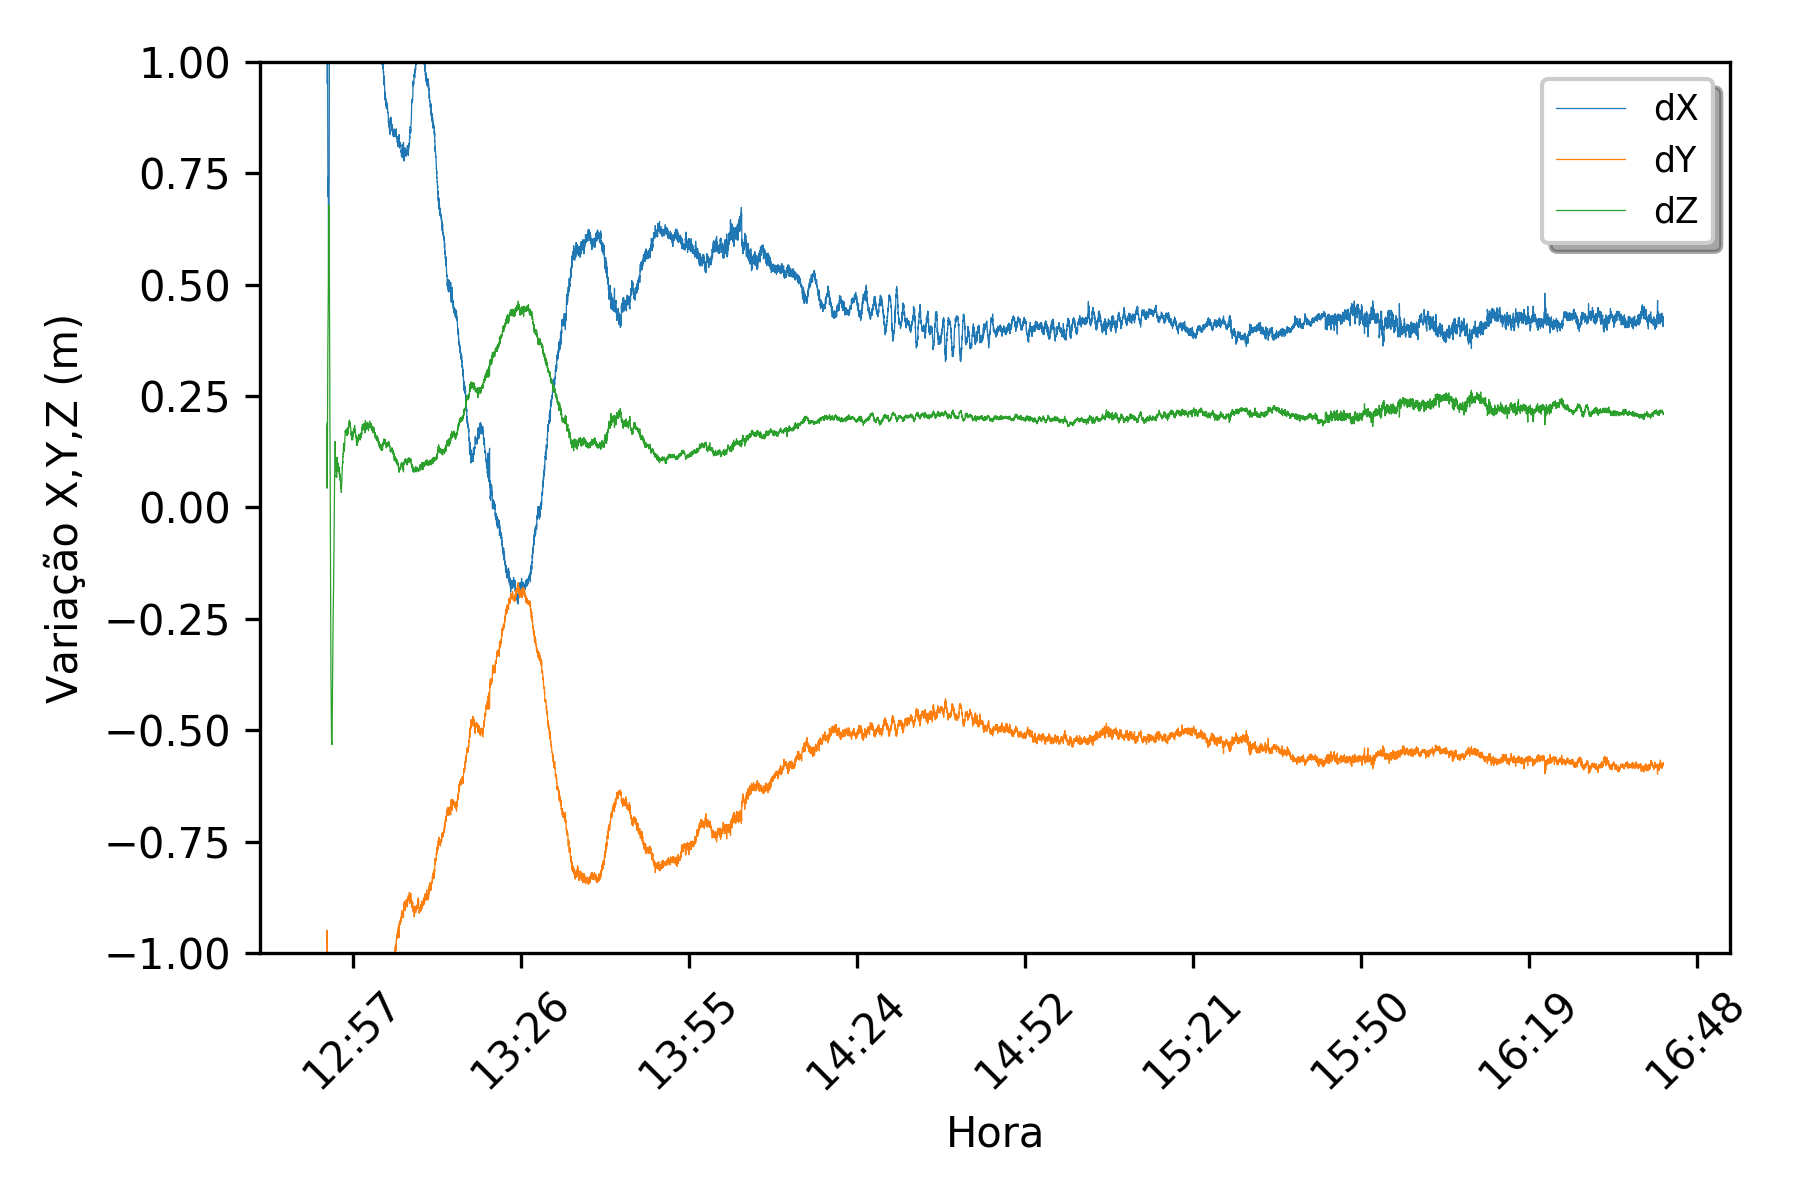
\includegraphics[scale=0.9]{data/Graphics/RJ_T20712/RJ_T20712_graphic_xyz.png}
\caption{Série temporal RTPPP - Resultante dX, dY, dZ.}
\label{}
\end{figure}

As coordenadas utilizadas como referências para o cálculo de dX, dY e dZ foram obtidas a partir da atualização das coordenadas obtidas no descritivo da estação do IBGE. As coordenadas atualizadas são: X = 4285796.90510288, Y = -4019920.95100773, Z = -2472249.93687366.

\begin{figure}[H]
\centering
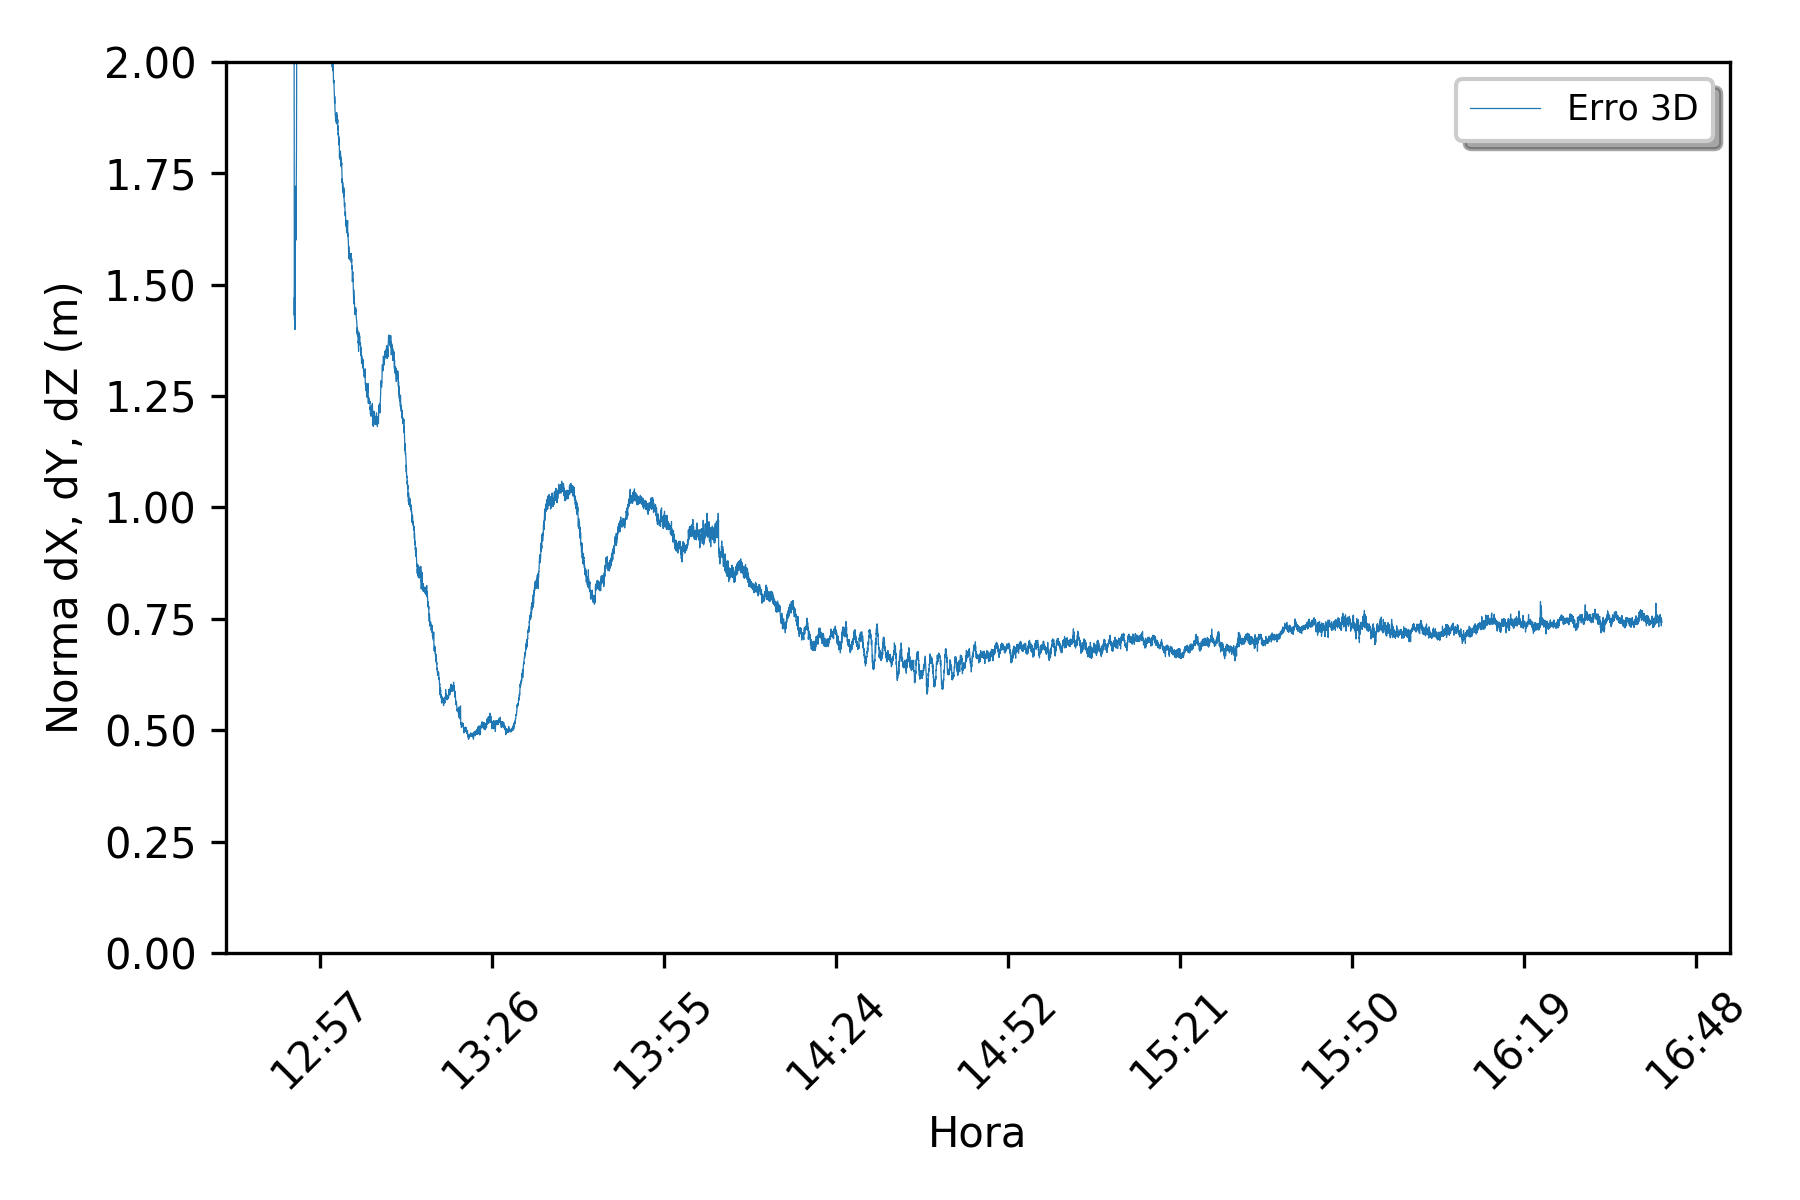
\includegraphics[scale=0.9]{data/Graphics/RJ_T20712/RJ_T20712_graphic_result.png}
\caption{Série temporal RTPPP - Norma de dX, dY, dZ.}
\label{result_20712}
\end{figure}

Na figura \ref{result_20712} é possível observar a resultante de dX, dY e dZ.

\begin{figure}[H]
\centering
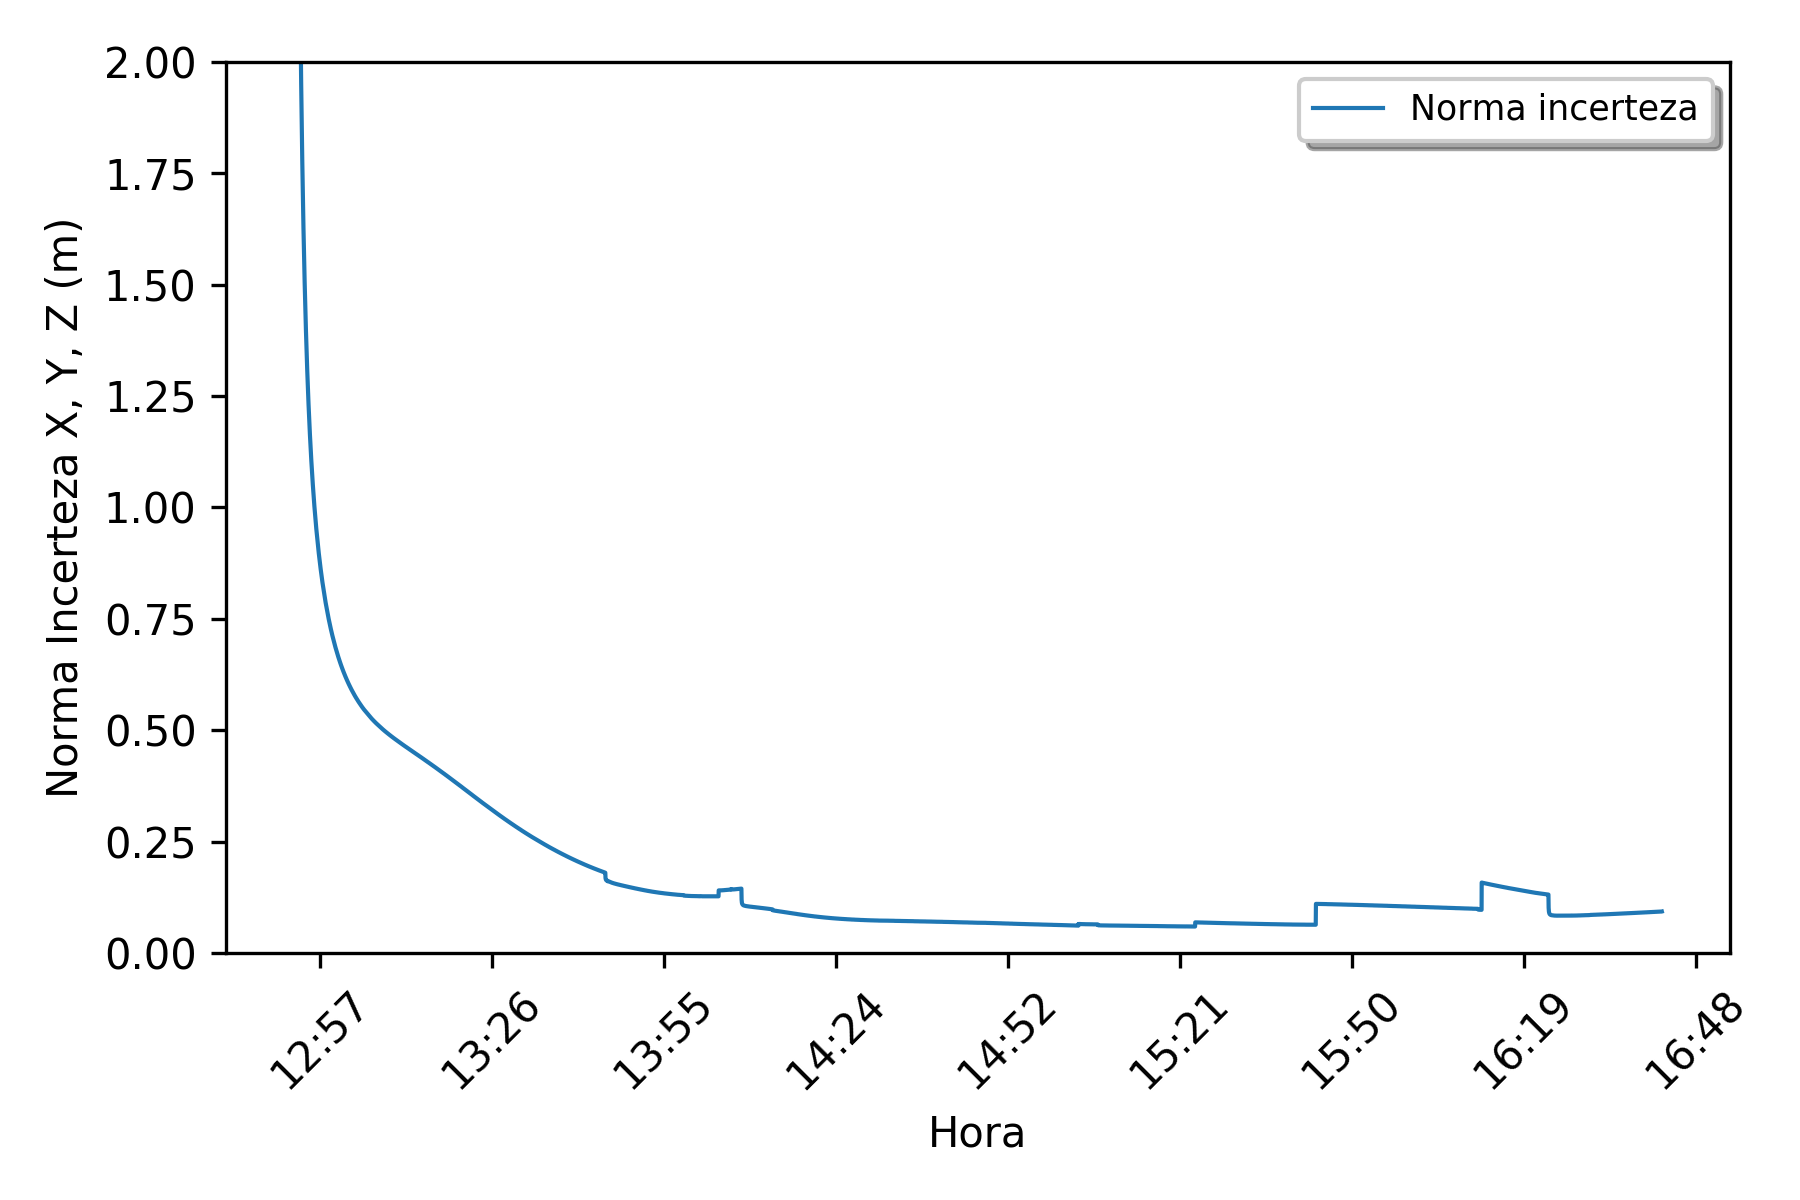
\includegraphics[scale=0.9]{data/Graphics/RJ_T20712/RJ_T20712_graphic_uncertainty.png}
\caption{Série temporal RTPPP - Incerteza das coordenadas X, Y, Z.}
\label{incerteza_20712}
\end{figure}

Na figura \ref{incerteza_20712} é possível observar que a resultante das incertezas converge para valores inferiores a 50 cm em torno de 10 a 15 minutos. Após uma hora a resultante varia de 10 a 20 cm.

Com o intuito de verificar a qualidade do levantamento realizado utilizou-se a ferramenta do IBGE de pós-processamento de dados GNSS \citep{ibge-ppp}, tal ferramenta se utiliza das efemérides ultra-rápidas, rápidas e finais para melhorar a acurácia do posicionamento. No processamento em questão os dados foram inseridos após 36 horas e menos de 11 dias do fim do rastreio, portanto o processamento utilizou-se de efemérides rápidas \citep{ibge_manual_ppp}. Os arquivos RINEX obtidos na medição foram utilizados para o processamento. Com o resultado do processamento comparou-se as coordenadas cartesianas época a época com as coordenadas obtidas em tempo real. A seguir os resultados:



\begin{figure}[H]
\centering
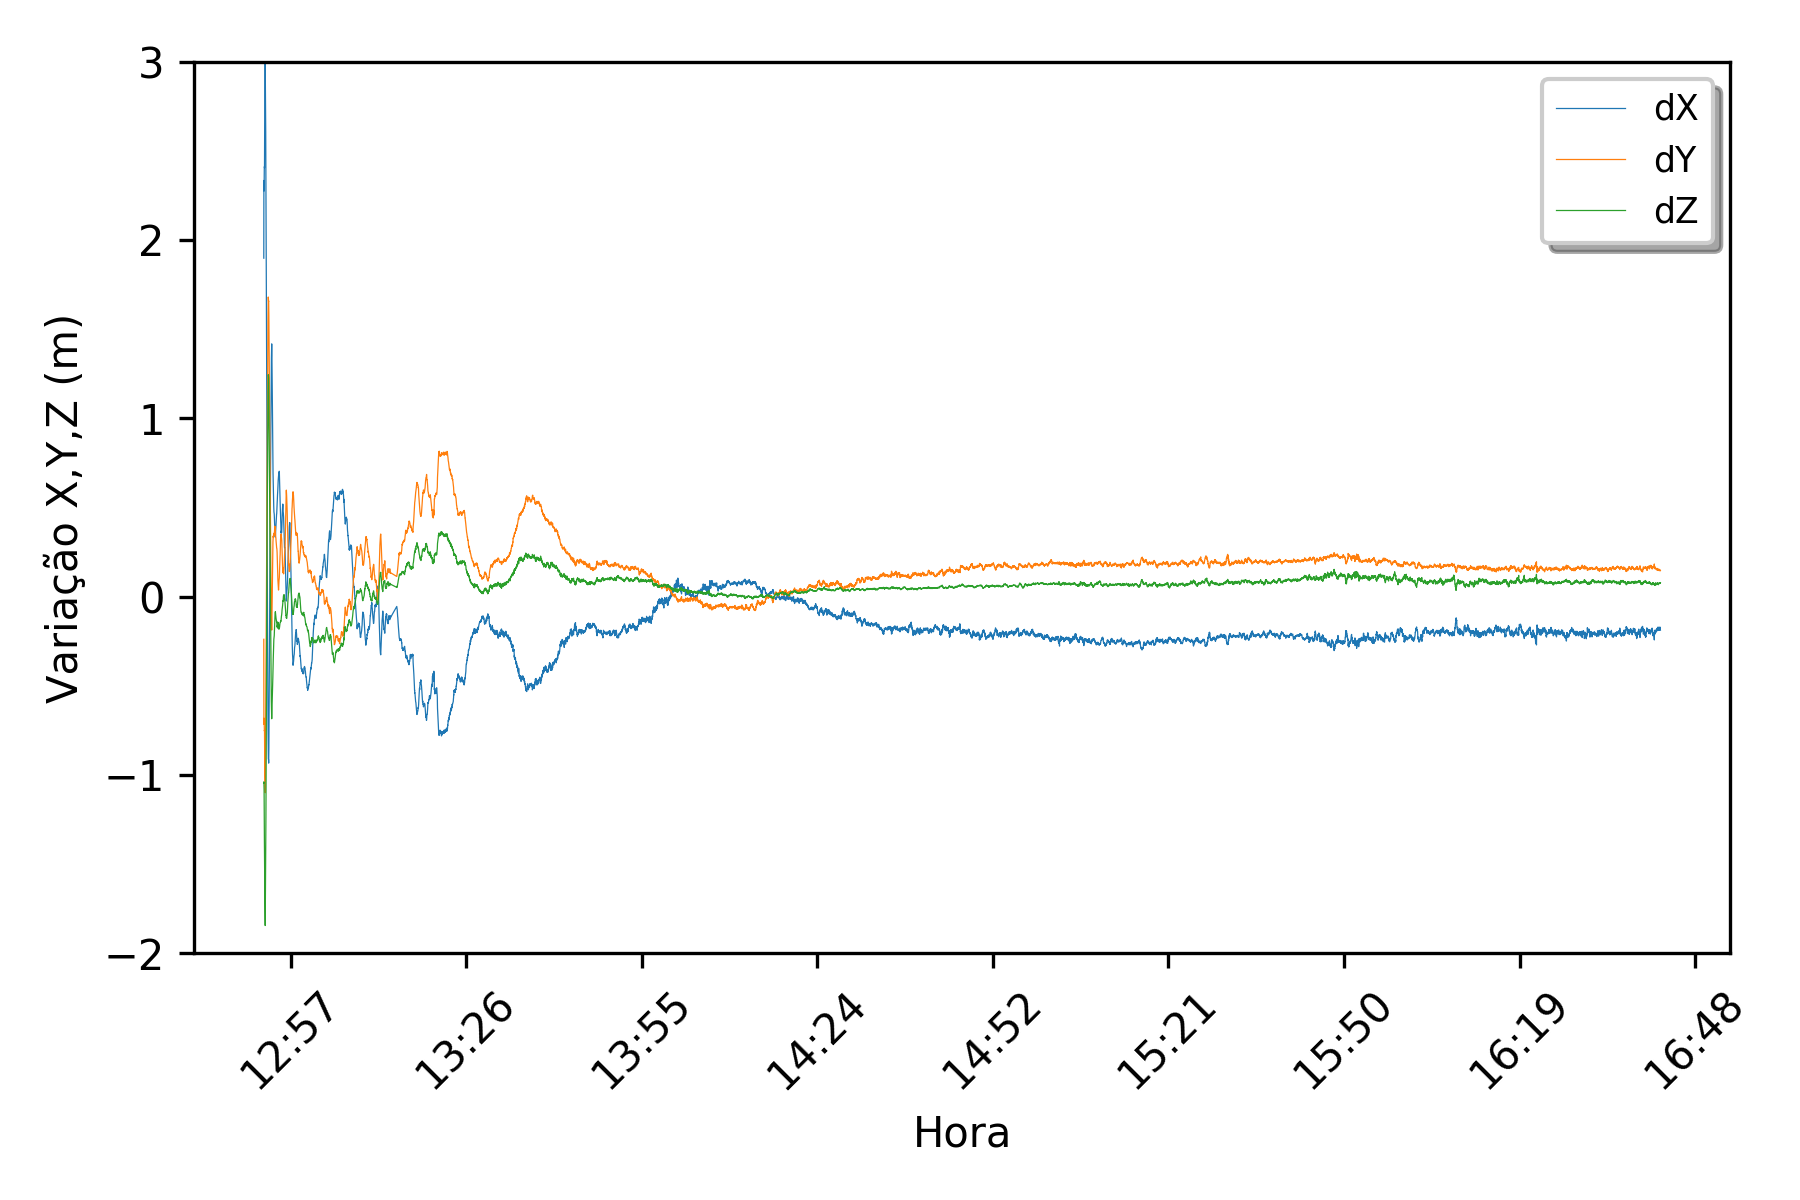
\includegraphics[scale=0.9]{data/Graphics/RJ_T20712/RJ_T20712_comparison_graphic_xyz.png}
\caption{Resultante dX, dY, dZ - Tempo real em comparação com pós-processado do IBGE.}
\label{comp_xyz_20712}
\end{figure}


\begin{figure}[H]
\centering
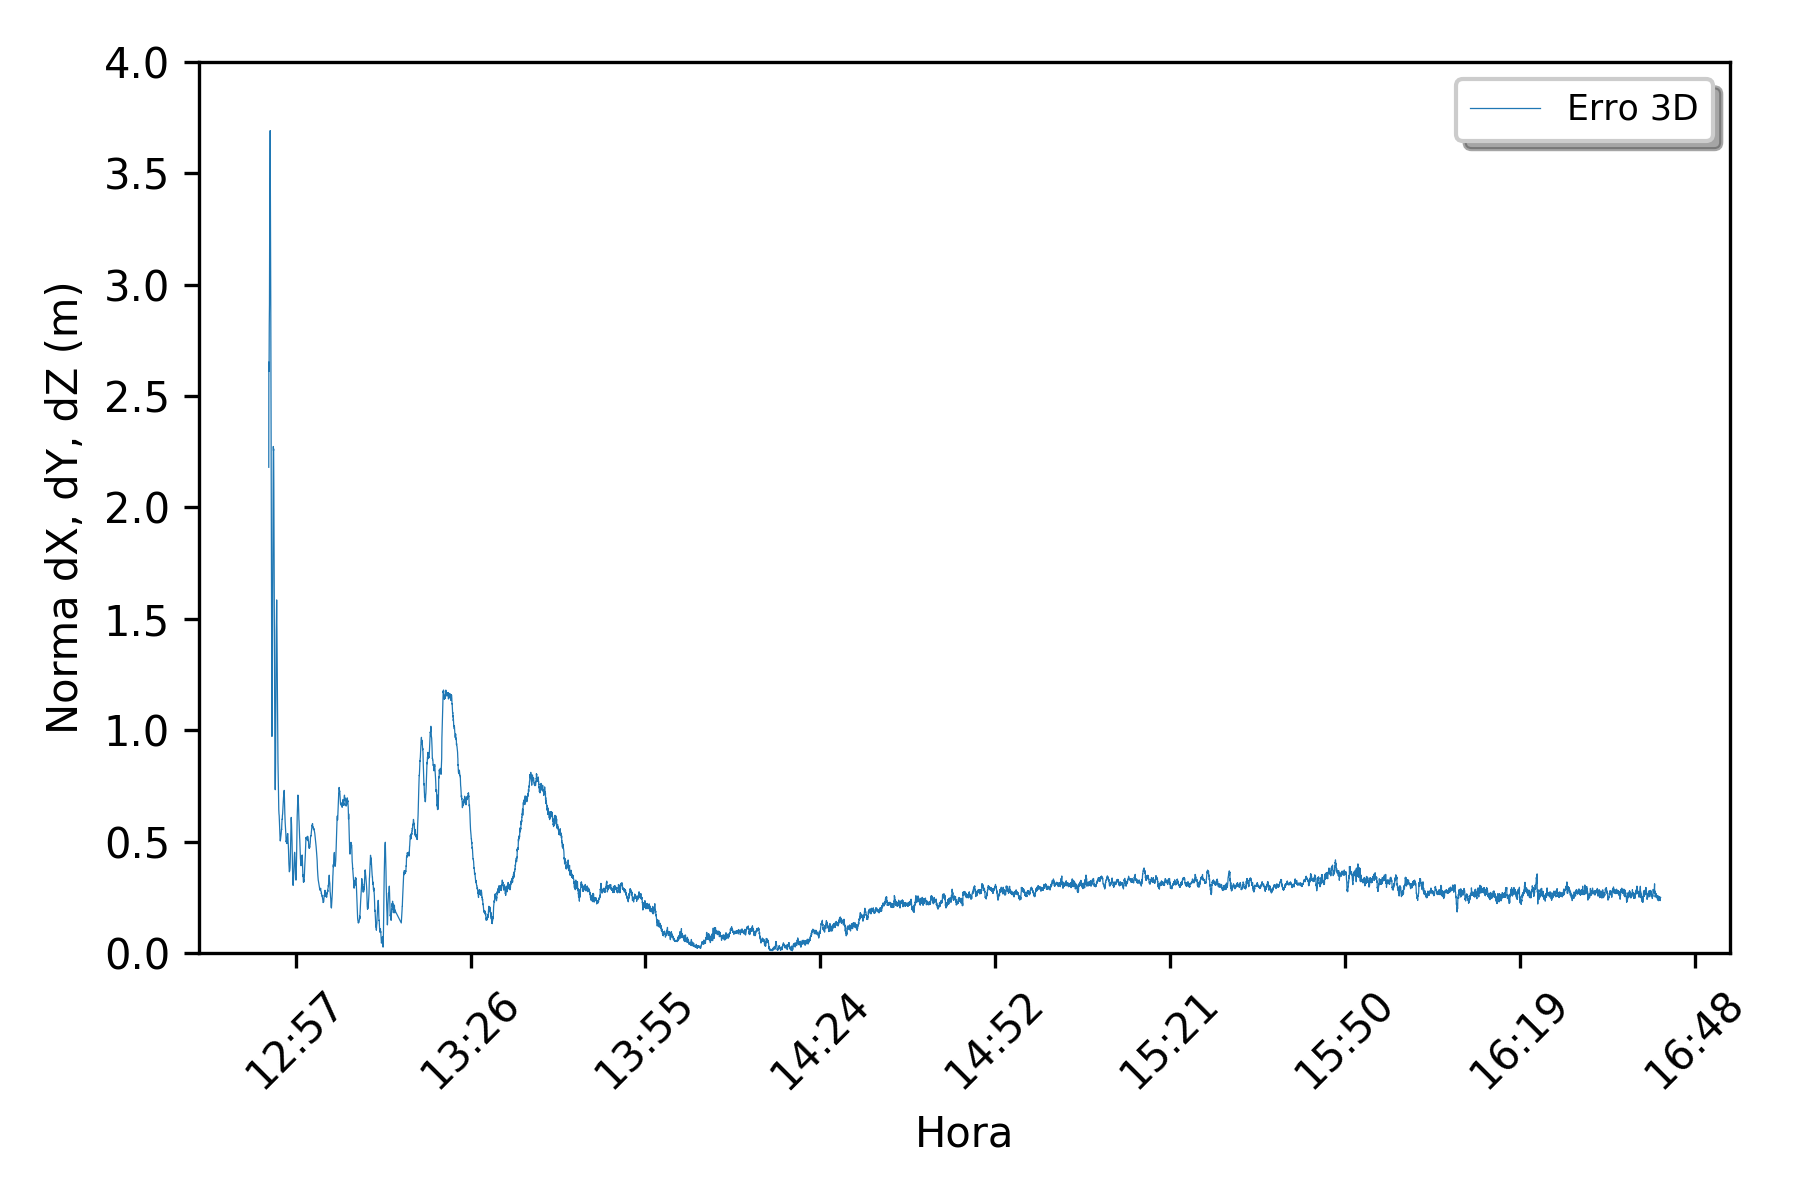
\includegraphics[scale=0.9]{data/Graphics/RJ_T20712/RJ_T20712_comparison_graphic_result.png}
\caption{Norma de dX, dY, dZ - Tempo real em comparação com pós-processado do IBGE.}
\label{comp_norma_20712}
\end{figure}

Pode-se observar na figura \ref{comp_xyz_20712} que os valores de dX, dY e dZ apresentam uma queda brusca de valores após os primeiros minutos de levantamento. Na figura \ref{comp_norma_20712} observa-se que na maior parte do levantamento, após uma hora de coleta, os valores da norma de dX, dY e dZ não são superiores a 50 cm.



\section{PPP-RTK}
Para a realização do método PPP-RTK utilizou-se o software ''PPP-Wizard''. Para fim de comparação entre o RTPPP, o qual utiliza solução \textit{float} de ambiguidades, e o PPP-RTK, o qual utiliza solução \textit{fixa} de ambiguidades, realizou-se, durante 24 horas, coleta de dados referente a estação POAL. A seguir os resultados:

\begin{figure}[H]
\centering
\subfigure[PPP-RTK\label{}]{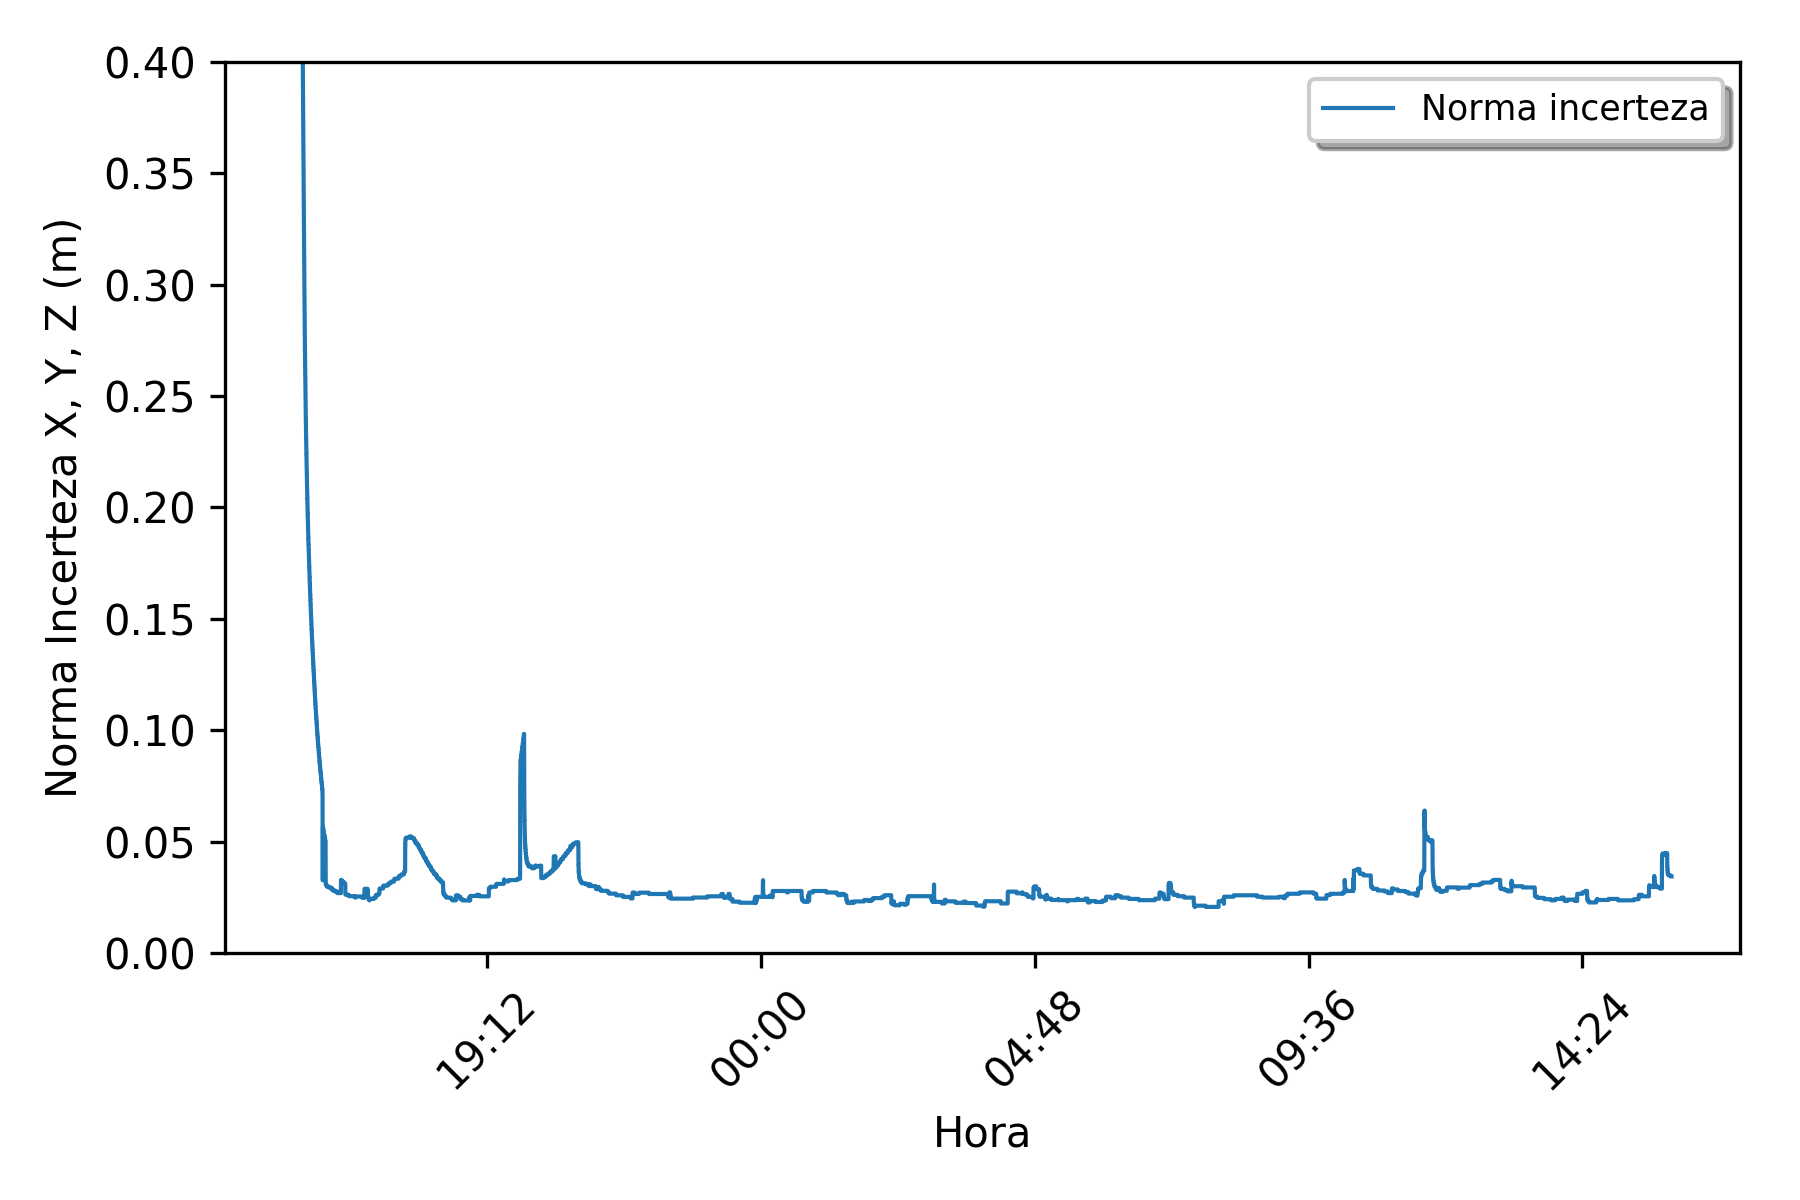
\includegraphics[scale=0.7]{data/Graphics/POAL001_ppp_wizard/POAL001_ppp_wizard_graphic_uncertainty.png}}
\subfigure[RTPPP\label{}]{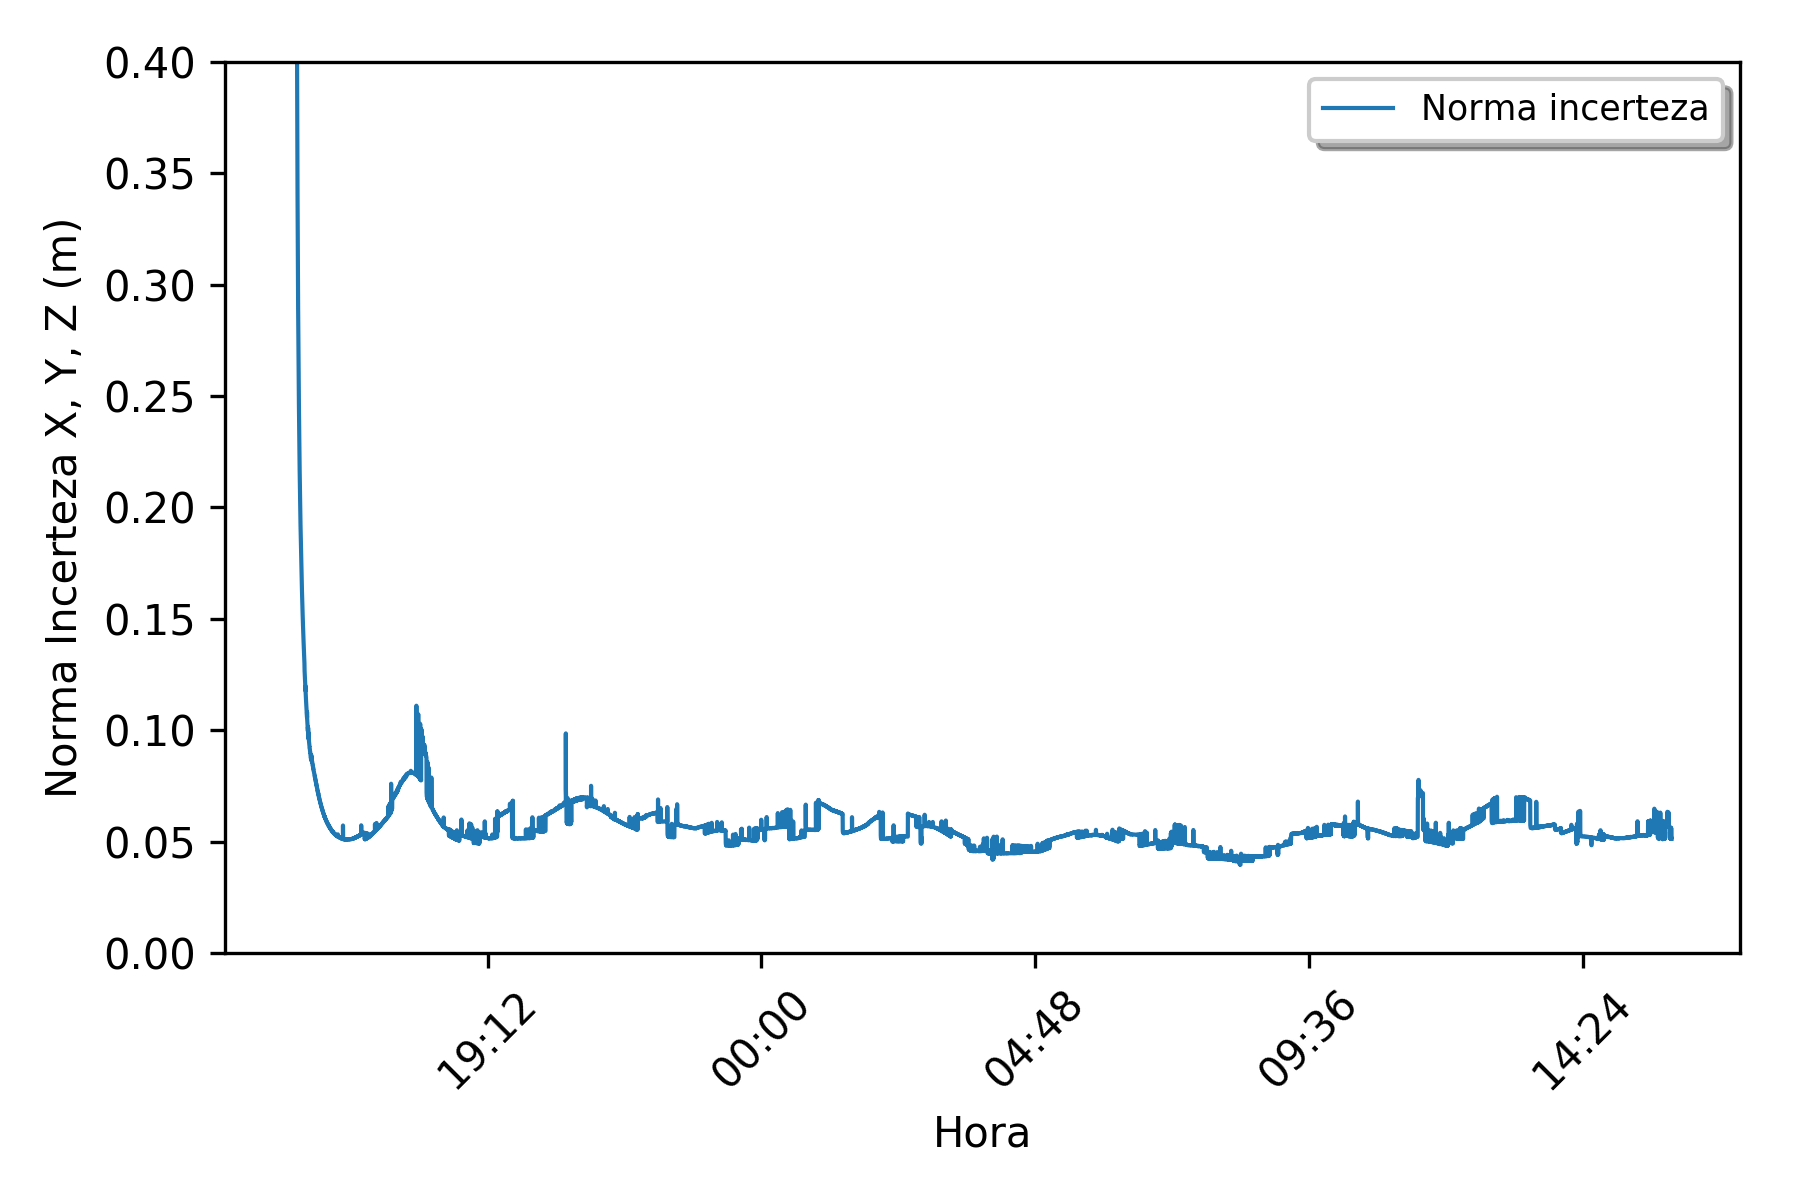
\includegraphics[scale=0.7]{data/Graphics/POAL20716/POAL20716_graphic_uncertainty.png}}
\caption{Comparação das incertezas entre RTPPP e PPP-RTK}
\label{comparacao_incert}
\end{figure}

Pode-se observar na figura \ref{comparacao_incert} que, como esperado, a resultante incerteza varia em valores menores quando se utilizada a solução fixa de ambiguidades. Ao utilizar-se o método PPP-RTK os valores variam menos e em torno de 3 cm, enquanto que no RTPPP os valores variam acima de 5 cm e apresentam maior variação.

\begin{figure}[H]
\centering
\subfigure[PPP-RTK\label{}]{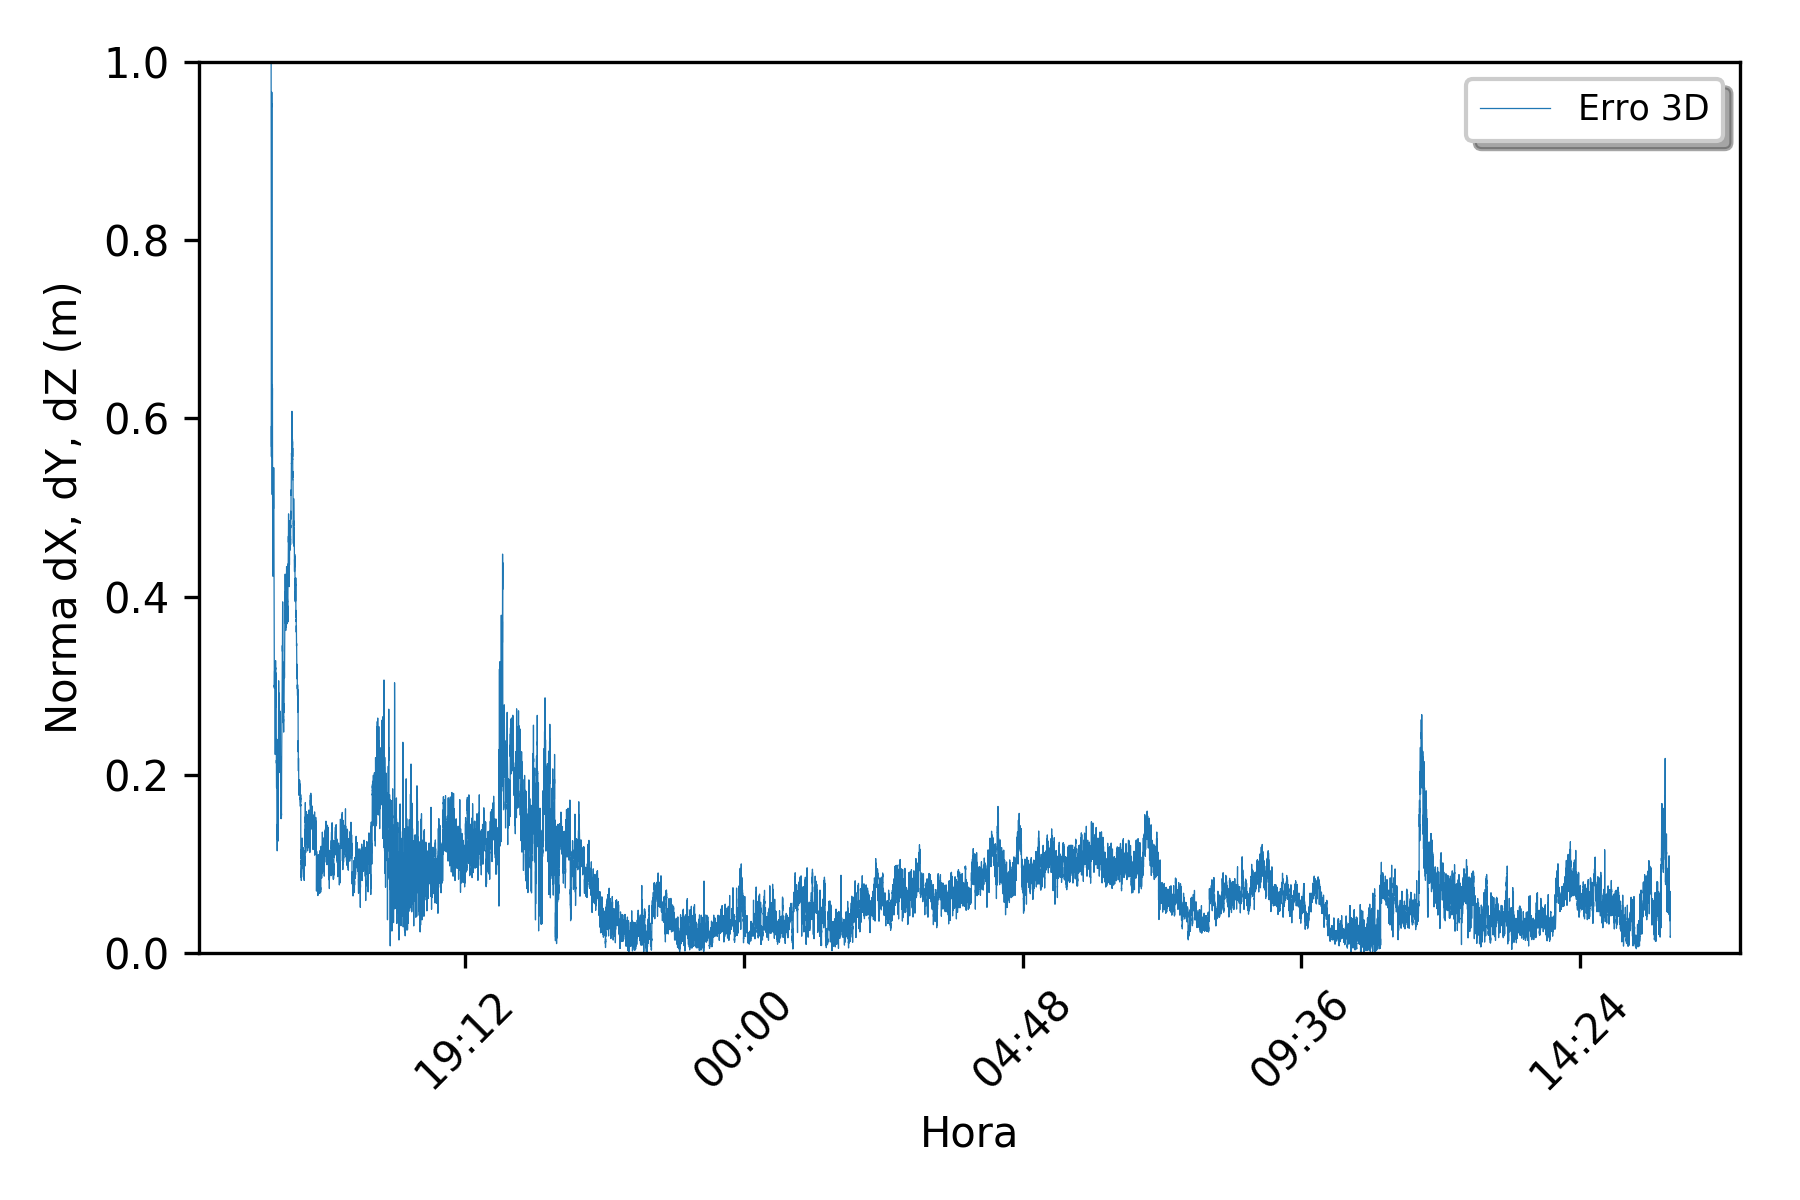
\includegraphics[scale=0.7]{data/Graphics/POAL001_ppp_wizard/POAL001_ppp_wizard_graphic_result.png}}
\subfigure[RTPPP\label{}]{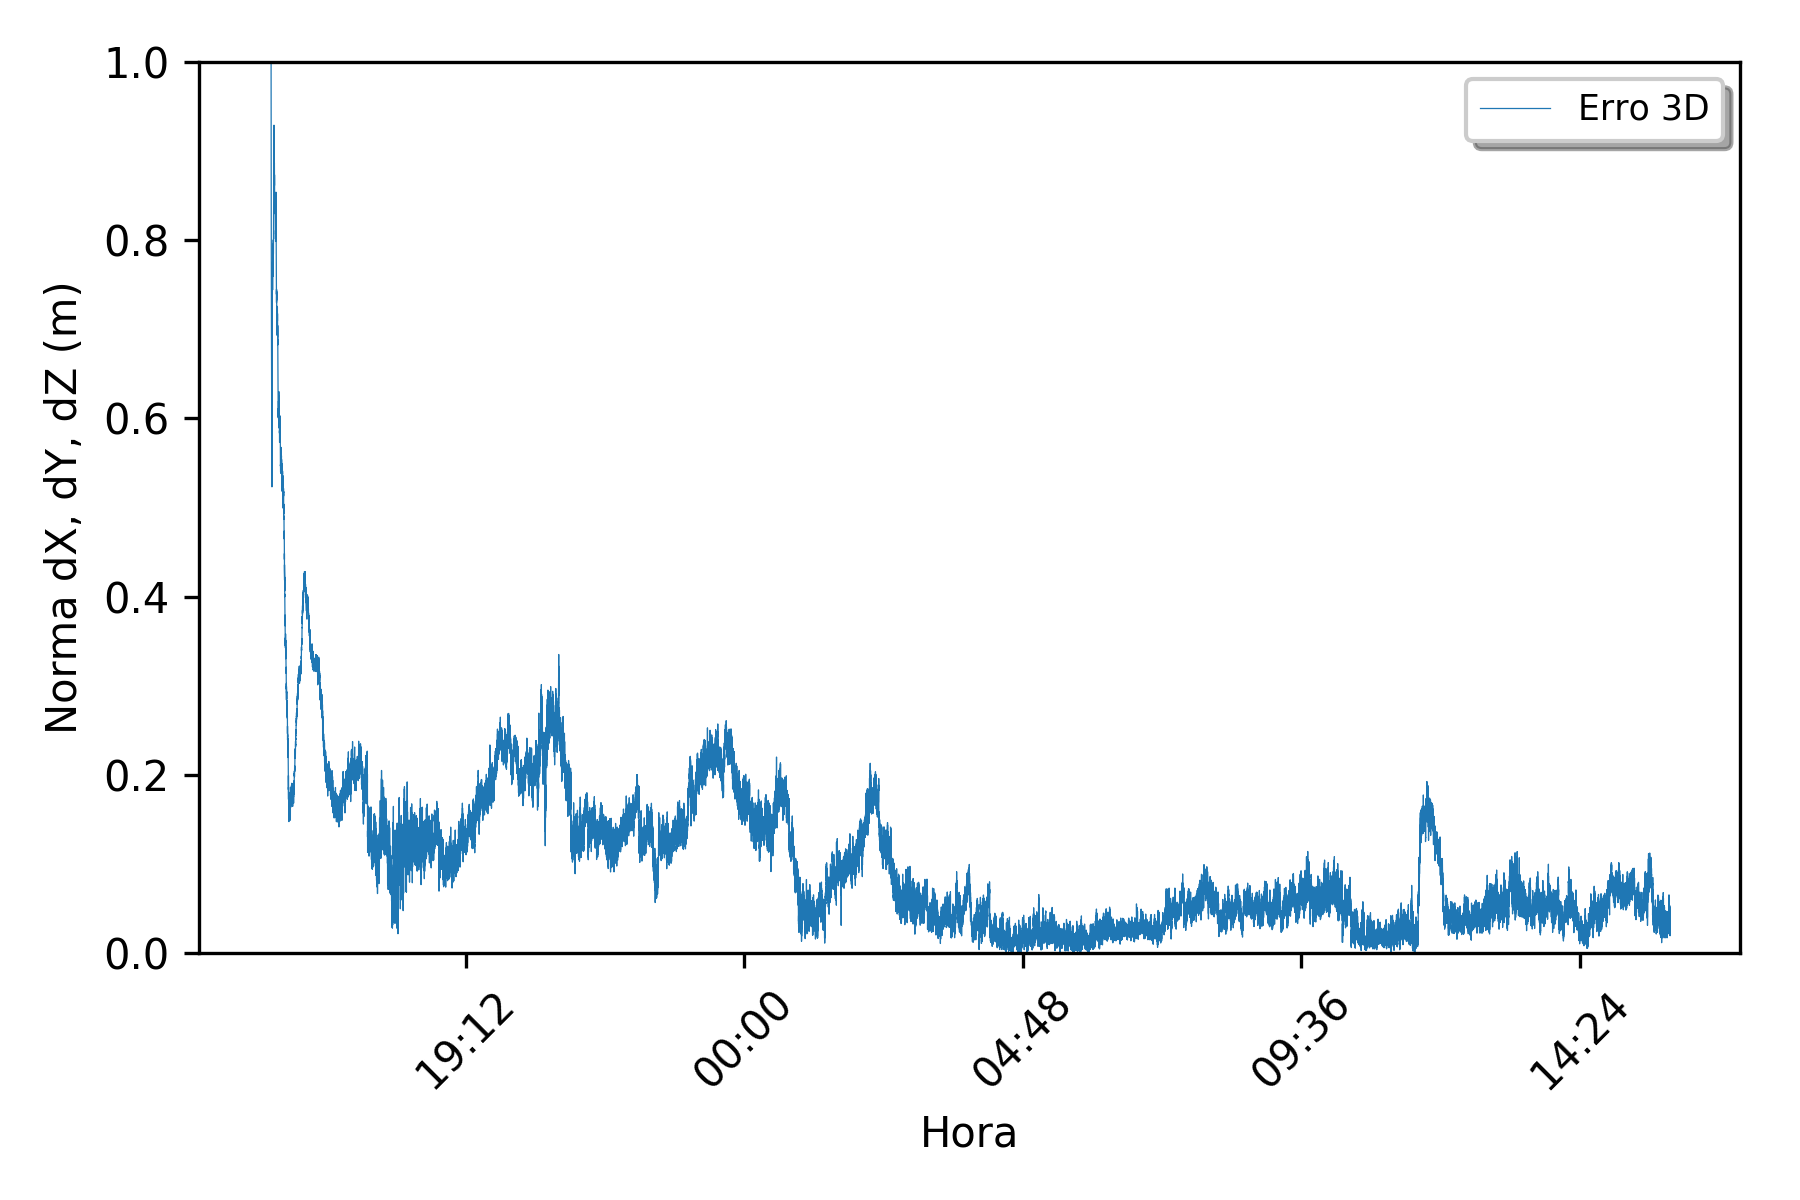
\includegraphics[scale=0.7]{data/Graphics/POAL20716/POAL20716_graphic_result.png}}
\caption{Comparação normas de dX, dY e dZ entre RTPPP e PPP-RTK}
\label{comparacao_xyz}
\end{figure}

Na figura \ref{comparacao_xyz} é possível observar que ao utilizar o RTPPP a resultante de dX, dY e dZ é ligeiramente maior que ao utilizar o PPP-RTK.

\section{RTK}
Com o objetivo de realizar as primeiras configurações no receptor GR-5, bem como entender corretamente seu funcionamento, realizou-se um RTK no prédio frontal do Instituto Militar de Engenharia, foram obtidos os pontos conforme figura a seguir:

\begin{figure}[H]
\centering
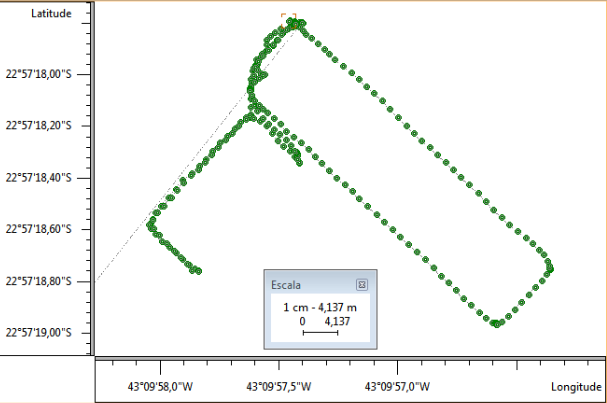
\includegraphics[scale=0.55]{img/rtk/mapa_rtk.png}
\caption{Pontos obtidos com levantamento RTK.}
\label{}
\end{figure}

A fim de avaliar a acurácia do RTK, gerou-se um gráfico com os erros médios quadráticos de cada ponto levantado:

\begin{figure}[H]
\centering
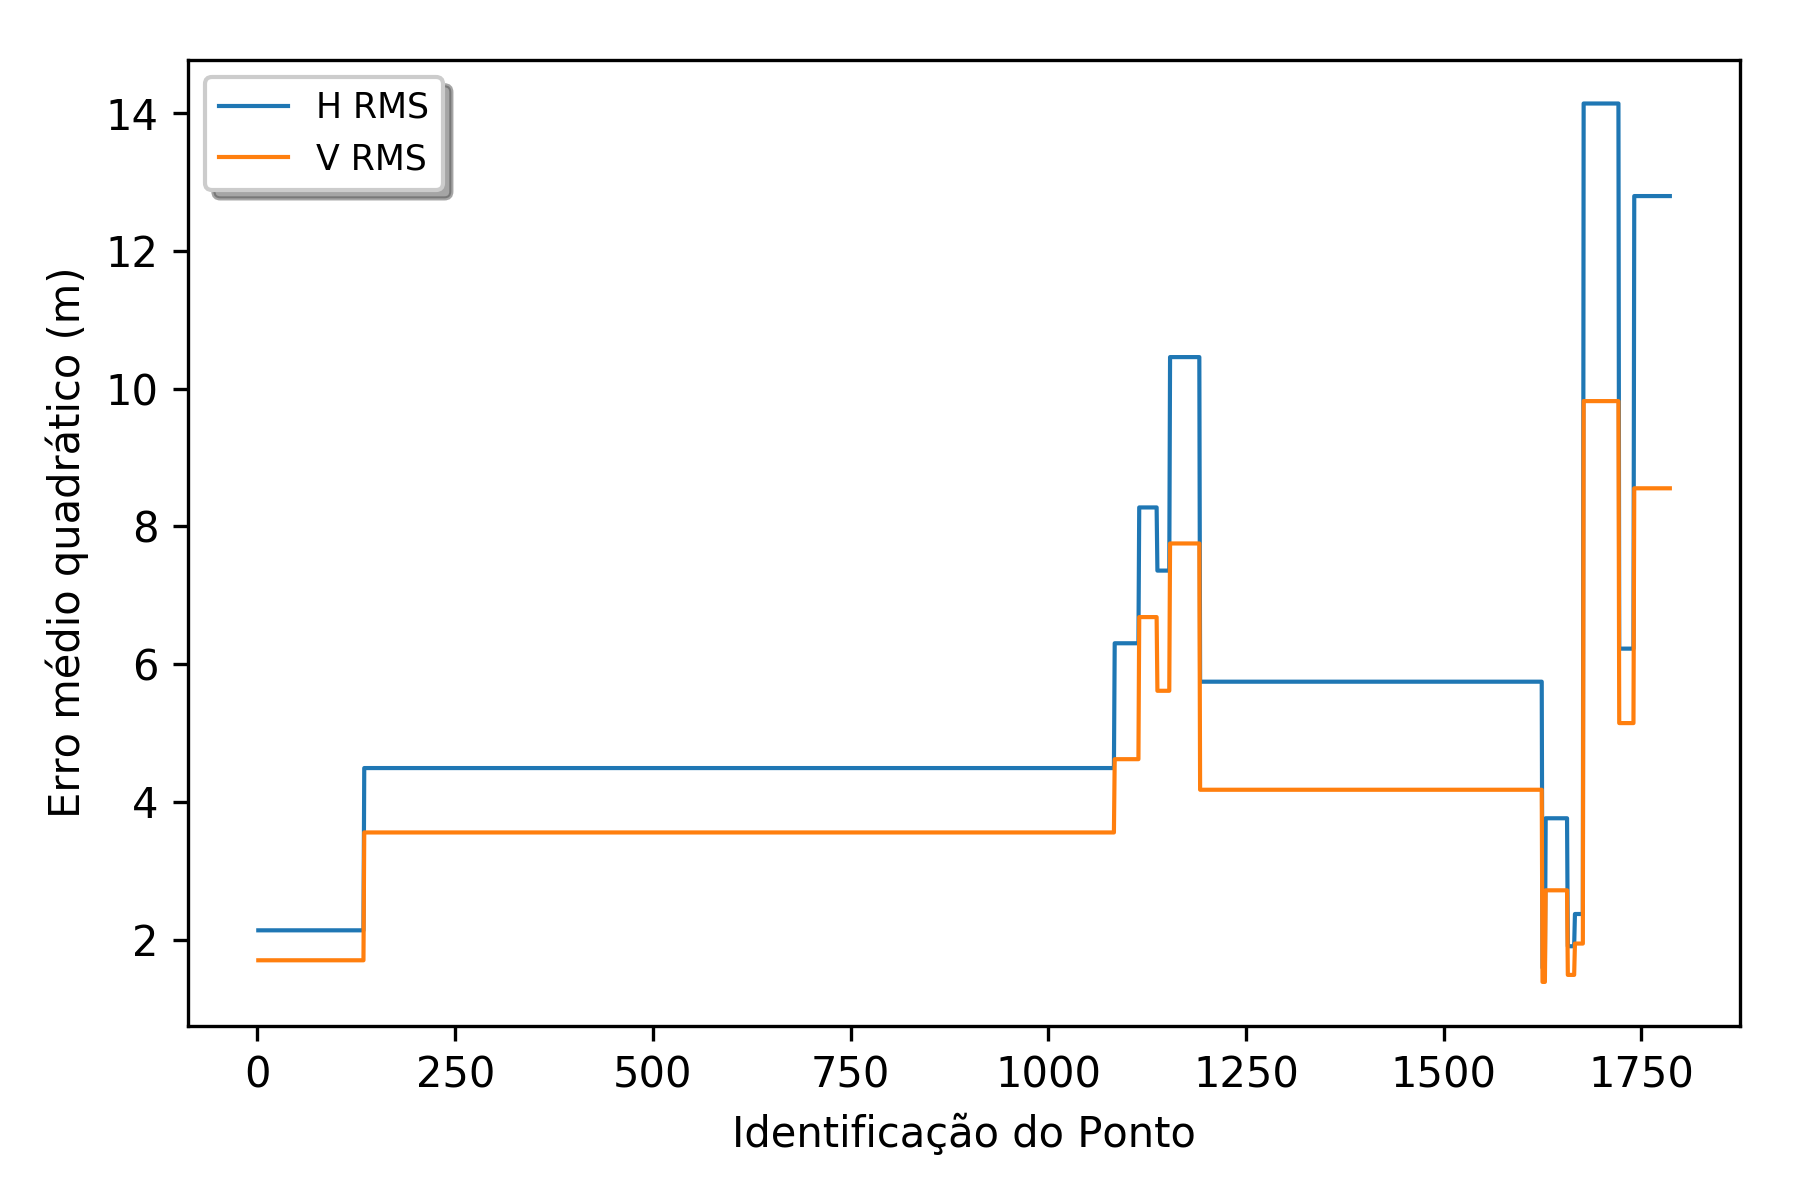
\includegraphics[scale=0.8]{img/rtk/rtk_rms.png}
\caption{Erro médio quadrático nas componentes Horizontal e Vertical.}
\label{rms_rtk}
\end{figure}

Observa-se na fig. \ref{rms_rtk} que os erros médios quadráticos atingiram valores acima do esperado para um posicionamento RTK. A verificação da causa de tal resultado será feita no seguimento do Projeto, visando demonstrar a viabilidade dos métodos de posicionamento GNSS em tempo real e facilitar a realização dos métodos PPP-RTK e RTP/NTRIP.






\chapter{Conclusão}

O desenvolvimento deste projeto gerou especificações técnicas e instruções para a realização dos métodos RTPPP, PPP-RTK e RTK com ferramentas de softwares livres e com receptor GNSS GR-5. Além disso, \textit{scripts} foram implementados para a extração das informações geradas por tais softwares possibilitando uma melhor visualização e análise dos dados. Tais especificações e códigos encontram-se no apêndice deste projeto. A análise aprofundada dos métodos de posicionamento espacial tratados neste projeto, apura a aplicação da teoria no mundo real além de demonstrar sua eficácia em relação à acurácia esperada e atendida. 

O RTPPP realizado em uma estação da RBMC mostrou que a incerteza das coordenadas permanece em valores inferiores a 10 cm e sua convergência para tais valores foi aproximadamente 40 minutos. Além da utilização da estação da RBMC, fez-se um RTPPP com o receptor GNSS conectado via porta serial e tal atividade gerou o conhecimento para realizar a conexão da maneira correta e eficiente; as orientações para realizar essa conexão se encontram nos apêndices deste projeto. Os valores das incertezas das coordenadas e tempo de convergência são similares ao levantamento RTPPP realizado com a estação da RBMC. Ao realizar o RTPPP com estação cinemática evidenciou-se sua operacionalidade e sua realização inteiramente com ferramentas livres. Ao comparar as coordenadas obtidas com as pós-processadas na ferramenta IBGE-PPP tem-se que no levantamento estático a resultante da diferenças das coordenadas apresenta valores próximos a 30 cm na maior parte do tempo, enquanto que no levantamento cinemático a mesma comparação apresenta valores próximos a 2 m (valores altos devidos o pouco tempo de levantamento que não possibilitou a devida convergência).

O PPP-RTK realizado em comparação com o RTPPP mostra que sua convergência é mais rápida, além de possuir valores de incerteza pŕoximos a 3 cm, enquanto que o RTPPP possui 5 cm. Tal fato dá-se em função da utilização da solução fixa de ambiguidades do PPP-RTK e não da solução \textit{float} de ambiguidades (RTPPP). Ainda, a realização do RTK ''clássico'' possibilitou a geração de informações que auxiliam e agilizam a configuração do receptor GR-5 (apêndice).


 As dificuldades encontradas foram amplamente analisadas e solucionadas na medida do possível, como as configurações dos receptores desde o início, a aquisição de materiais para a conexão (cabos) e o entendimento do funcionamento dos métodos. Outras dificuldades exploradas não tiveram solução completa, como a questão do recebimento de dados pelo receptor por meio de internet 4G via ''\textit{SIM card}'' e um novo levantamento RTK. Por questões de gestão de tempo e priorização dos objetivos principais, estas tarefas podem ser exploradas em trabalhos futuros, valendo-se do escopo deste trabalho. A realização deste projeto materializa a possibilidade de utilizar meios modernos (receptores recém lançados) e acessíveis (plataformas e softwares livres) para as diversas empregabilidades citadas
Assim, o anseio de aplicar produtos GNSS em projetos de engenharia é crescente e factível para trabalhos futuros para explorar outros detalhes não abordados no presente relatório.
%%
%
% ARQUIVO: apendice.tex
%
% VERSÃO: 1.0
% DATA: Maio de 2016
% AUTOR: Coordenação de Trabalhos Especiais SE/8
% 
%  Arquivo tex de exemplo de apêndice do documento de Projeto de Fim de Curso.
%  Este exemplo traz dois apêndices (dois comandos \chapter{•}). Poderiam ser colocados em arquivos .tex
%  separados. Neste caso, o arquivo main.tex deveria ter um \include{•} para cada arquivo .tex
%
% ---
% DETALHES
%  a. todo apêndice deve começar com \chapter{•}
%  b. usar comando \noindent logo após \chapter{•}
%  c. segue os mesmos DETALHES do arquivo .tex de exemplo de capítulo do documento de Projeto de Fim de Curso
% ---
%%


\chapter{Apêndice A - Configurações}
\noindent

\section{Configurações do BNC}
\label{bnc_config}

Para a realização do método RTPPP utilizando o software BNC, uma série de configurações devem ser estabelecidas. A seguir, elas são detalhadas:

\begin{itemize}
    \item General
    \begin{itemize}
        \item \textit{Logfile (fullpath)} - Deve se indicar o caminho onde o Log do RTPPP será salvo. Recomenda-se criar uma pasta ''LOG'' para tal função. Os arquivos Log são importantes pois neles é que são registradas as coordenadas de cada época, entre outras informações.
        \item \textit{Re-read configuration} - Recomenda-se deixar desabilitada essa opção pois caso ela esteja habilitada e o usuário alterar as configurações e iniciar o levantamento, quando as configurações forem re-lidas o levantamento pode parar devido a alteração feita logo antes do início.
    \end{itemize}
    \item \textit{RINEX Observations}
    \begin{itemize}
        \item \textit{Directory} - Deve se indicar o caminho para que se salvem os arquivos RINEX do levantamento. Recomenda-se criar uma pasta ''RINEX''. Caso o caminho não seja indicado os arquivos não serão salvos e não será possível pós processar os dados do levantamento.
        \item \textit{Interval} - Tempo que se deseja para salvar o arquivo RINEX. Caso seja ''2 horas'', o software salva um arquivo RINEX a cada duas horas.
        \item \textit{Sampling} - Amostragem das épocas. Caso seja ''1 segundo'' o software calcula e salva uma coordenada por segundo.
    \end{itemize}
    \item \textit{RINEX Ephemerides}
    \begin{itemize}
        \item Análogo a aba \textit{''RINEX Observations''} mas para as Efemérides.
    \end{itemize}
    \item \textit{PPP} (1) - Nesta aba são determinadas as principais configurações do RTPPP
    \begin{itemize}
        \item \textit{Data source} - \textit{Real-Time Streams}
        \item \textit{Corrections stream} - Determina qual o stream utilizado para receber as correções para o PPP em tempo real. Nesse trabalho foi utilizado o ''CLK91''.
        \item \textit{Coordinates file} - Indica-se o caminho para o arquivo que contém as coordenadas da estação que está sendo levantada, naturalmente as coordenadas podem ser aproximadas e são utilizadas para que o programa estime um dE, dN e dU e a visualização da convergência seja facilitada. Ainda neste arquivo deve-se constar o modelo da antena utilizada de acordo com o padrão do arquivo de antenas do IGS. A seguir o extrato completo do arquivo utilizado em um dos levantamentos: "POAL00BRA0  3467519.42758  -4300378.65527  -3177517.52025  0.0000  0.0000  0.0010 TRM115000.00    NONE TRIMBLE NETR9''.
        \item \textit{Logfile directory} - Indica-se para a pasta onde os log's serão salvos.
        \item \textit{ANTEX file} - Caminho para o arquivo que contém as especificações das antenas.
    \end{itemize}
    \item \textit{PPP} (2) -  Deve-se adicionar o nome da estão exatamente como está escrito no arquivo de coordenadas e na lista de streams.
    \item \textit{PPP} (3) - Opções sobre as portadoras e os sistemas GNSS - convém utilizar ''P3 \& L3'' sempre que possível.
    \item \textit{PPP} (4)
    \begin{itemize}
        \item \textit{PPP Plot} - Deve-se inserir o nome da estação que se deseja plotar o gráfico para visualização.
    \end{itemize}
    \item \textit{Add Stream} (figura \ref{add_stream}) - Nesse botão é onde são incluídos os streams para as correções e recebimento das observáveis GNSS.
    \begin{itemize}
        \item Correções - Para as correções e efemérides foram utilizados dois \textit{streams}, ambos no \textit{Caster host} ''\textit{products.igs-ip.net}'', porta 2101. Os streams foram: ''CLK91'' e ''RTCM3EPH''.
    \end{itemize}
\end{itemize}

\begin{figure}[H]
\centering
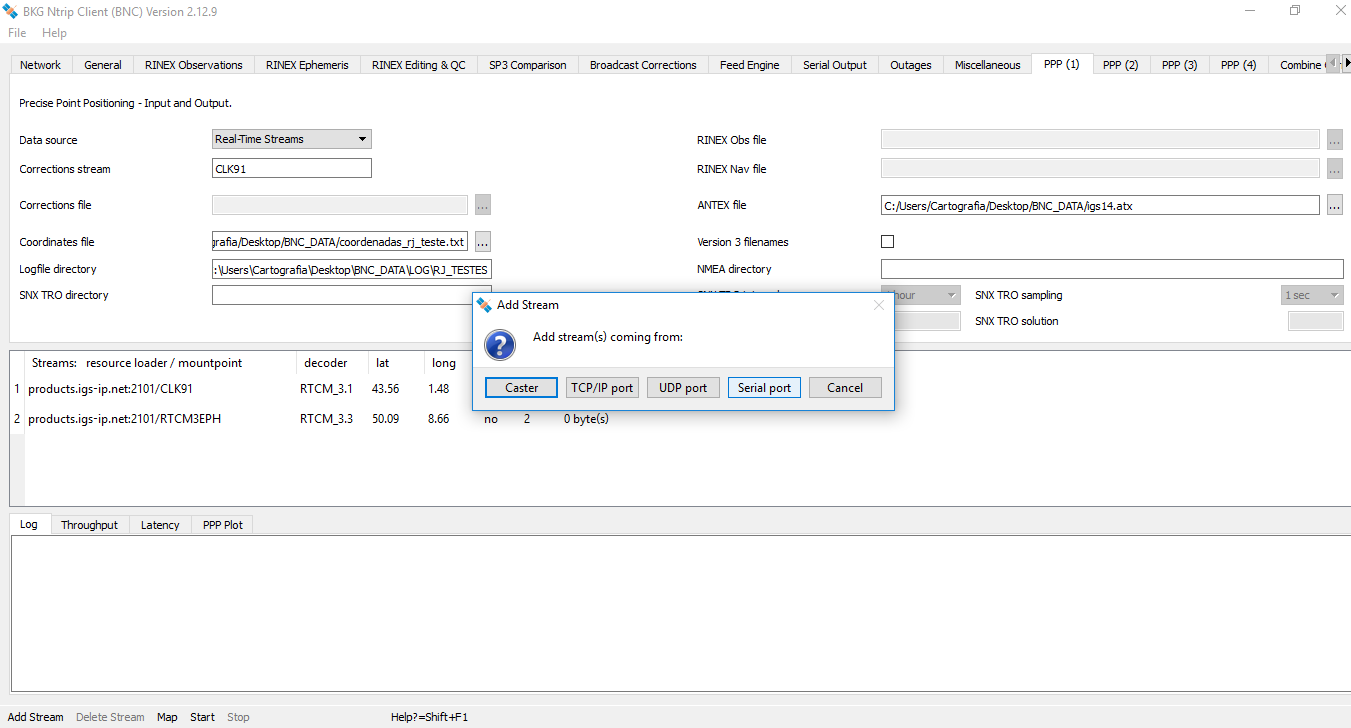
\includegraphics[scale=0.4]{img/BNC_18.png} %scale eh o tamanho que a figura vai ficar
\caption{Adição de stream \textit{stream}.}
\label{add_stream}
\end{figure}

\subsection{RTPPP com recebimento de dados do receptor via caster}
\label{rtppp_caster_bnc}
Para realizar o RTPPP dessa forma realiza-se a configuração conforme seção \ref{bnc_config} e inclui-se outro stream da seguinte forma:
\begin{itemize}
    \item \textit{Add Stream}
    \begin{itemize}
        \item \textit{Caster} - \textit{Caster host} ''\textit{www.igs-ip.net}'', porta 2101. O stream utilizado nesse trabalho foi: ''POAL00BRA0''.
    \end{itemize}
\end{itemize}



\subsection{RTPPP com recebimento de dados do receptor via porta serial}
\label{rtppp_serial_bnc}
Nesse trabalho a conexão Receptor - Computador foi feita utilizando dois cabos: Serial/COM (fêmea) e COM (Macho) - COM (Macho). O segundo cabo foi necessário pois foi um adaptador para a porta disponível no computador utilizado. Para realizar o RTPPP dessa forma realiza-se a configuração conforme seção \ref{bnc_config} e inclui-se outro \textit{stream} da seguinte forma:
\begin{itemize}
    \item \textit{Add Stream}
    \begin{itemize}
        \item \textit{Serial port} - A configuração utilizada nesse trabalho foi:
        \begin{itemize}
            \item \textit{Mountpoint} - ''RJ$_$teste'' - A denominação da \textit{Mountpoint} é de acordo com o usuário, devendo ser o mesmo dado no arquivo de coordenadas;
           \item \textit{Format} - ''RTCM$_$3'' - Formato que o BNC fará a leitura dos dados recebidos pelo receptor. É importante ressaltar que essa configuração deve estar coerente com a configuração dos dados de saída do receptor, nesse trabalho o receptor estava configurado para enviar dados no formato ''RTCM 3.x'';
            \item Latitude e Longitude - valores aproximados e inteiros, somente para exibição na lista da tela;
            \item \textit{Country} - País onde está localizado o receptor. Somente para fins de exibição em tela;
            \item \textit{Port name} - ''COM1'' - No sistema operacional Windows por padrão a porta ''COM'' é denominada ''COM1'' ou ''COM2'', vale ressaltar que no computador utilizado a cada vez que a conexão com o receptor era refeita o sistema criava um novo nome, como por exemplo ''COM6'' - Esse é o nome da porta em que o receptor está conectado via cabo.
            \item \textit{Baud rate} - 115200 - Recomenda-se que seja tão alta quanto possível.
            \item \textit{Data bits} - 8
            \item \textit{Stop bits} - 1
            \item \textit{Parity} - \textit{None}
            \item \textit{Flow control} - \textit{Off}
            \item As configurações de \textit{Baud rate}, \textit{Data bits}, \textit{Stop bits}, \textit{Parity}, \textit{Flow control} devem ser idênticas com a configuração estabelecida na saída de dados do receptor.
        \end{itemize}
    \end{itemize}
\end{itemize}

A figura \ref{bnc_stream_serial} explicita os passos explicados na seção \ref{rtppp_serial_bnc}:
\begin{figure}[H]
\centering
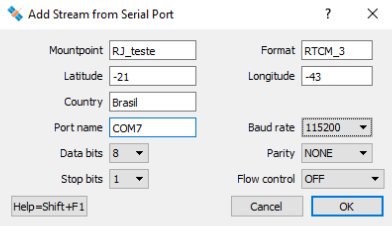
\includegraphics[scale=0.4]{img/BNC_19.png} %scale eh o tamanho que a figura vai ficar
\caption{Adição de stream via porta serial.}
\label{bnc_stream_serial}
\end{figure}

Realizadas as configurações explicadas nas seções \ref{bnc_config} e \ref{rtppp_caster_bnc} ou \ref{rtppp_serial_bnc}, aciona-se o botão \textit{start} para começar o recebimento e processamento de dados. A figura \ref{receb_dados_bnc} mostra tal recebimento.

\begin{figure}[H]
\centering
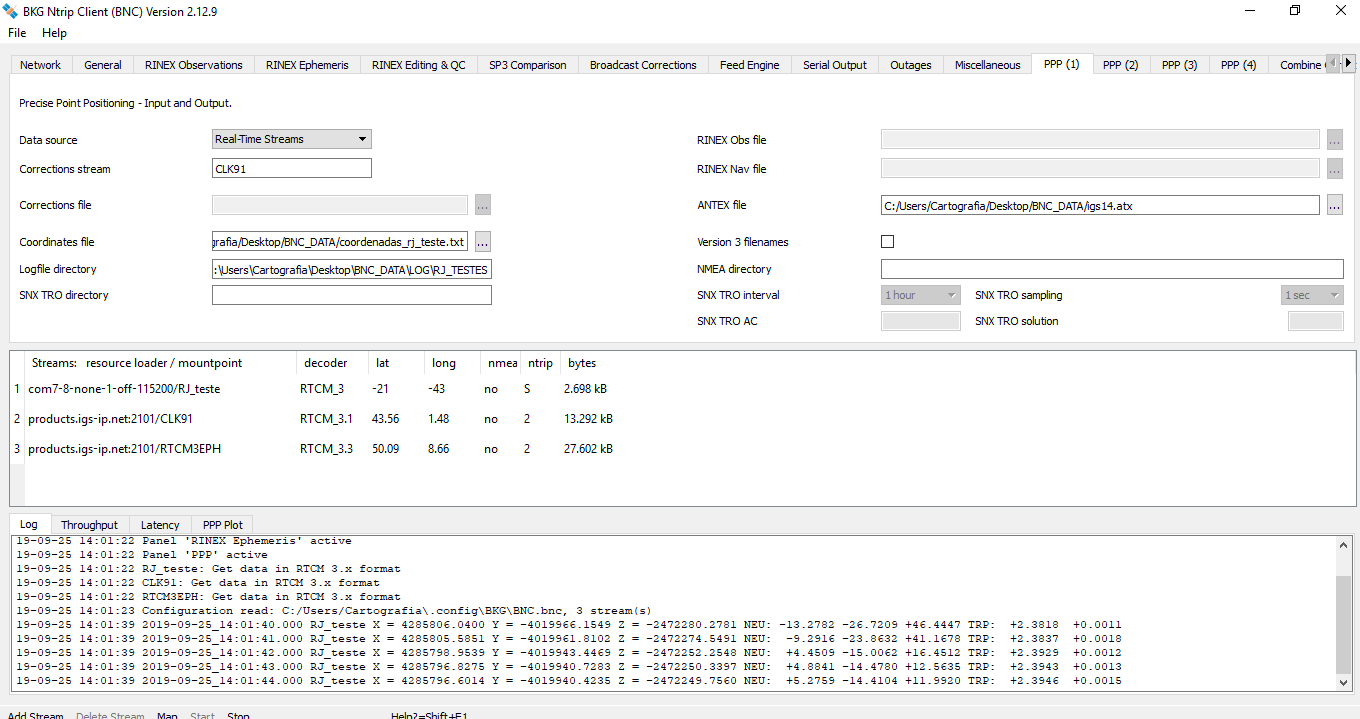
\includegraphics[scale=0.4]{img/BNC_21.png} 
\caption{Chegada de dados e processamento no BNC.}
\label{receb_dados_bnc}
\end{figure}

\section{Configuração do PPP-Wizard para realização do PPP-RTK}

Para a realização do PPP-RTK nesse trabalho utilizou-se o software PPP-Wizard, uma modificação do código do BNC que utiliza solução fixa de ambiguidades ao invés de solução \textit{float}. A seguir serão detalhados alguns passos para a configuração e utilização do PPP-Wizard.

Primeiramente deve-se abrir a pasta onde encontram-se os arquivos do programa diretamente no terminal (ou \textit{Prompt de comando}). Nessa pasta devem constar os seguintes arquivos básicos: \textit{conf\_get.txt}, \textit{conf\_process.txt} e \textit{rover.txt}.

O arquivo \textit{conf\_get.txt} especifica quais serão os \textit{streams} a serem conectados para o recebimento de dados e correções. A seguir o arquivo utilizado no presente projeto:

\lstinputlisting{PPPWizard141/conf_get.txt}

O usuário e senha devem ser obtidos através de cadastro no portal do IGS.

O arquivo \textit{conf\_process.txt} determina as opções do procedimento. É importante selecionar o modo \textit{mode\_PPP\_AR} e colocar o modelo da antena utilizada. A seguir um extrato do arquivo \textit{conf\_process.txt} utilizado:

\begin{lstlisting}
    mode_PPP_AR mode
    igs14.atx TRM115000.00
    1 1 0 AR/JumpsIndicators
    1 useGPS
    1 useGlonass
\end{lstlisting}

O \textit{rover.txt} informa o nome da estação e suas coordenadas aproximadas. A seguir o arquivo utilizado:
\lstinputlisting{PPPWizard141/rover.txt}

Após a manipulação desses três arquivos deve-se executar o seguinte comando no terminal:

\begin{lstlisting}
    ./getStream <conf_get.txt | ./processStream -conf conf_process.txt -rover rover.txt -dcb "*.DCB" > out_POAL_PPP_wizard.txt
\end{lstlisting}

O arquivo de saída \textit{out\_POAL\_PPP\_wizard.txt} armazenará todas as coordenadas e suas respectivas épocas.

\section{Configuração via \textit{software} TRU do Receptor (GR-5) para a comunicação com computador}

Esta seção explicará a configuração para a comunicação correta entre o receptor e computador, visando a utilização do \textit{software} BNC. A configuração é realizada através do \textit{software} TRU.

\begin{itemize}
    \item Conexão do receptor com \textit{software} TRU: \textit{Device > Connect}
    \item Seleciona-se a porta serial através do botão ''...'' e então pressiona-se o botão \textit{Connect}
\end{itemize}

\begin{figure}[H]
\centering
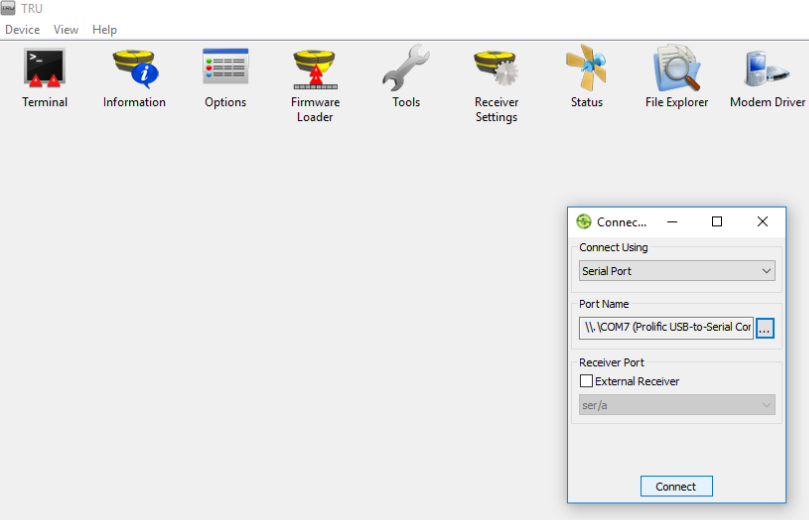
\includegraphics[scale=0.4]{pfc_pdf_files/img/TRU_3_conexao.png}
\caption{Identificação da conexão do receptor via porta serial.}
\label{Rotulo}
\end{figure}

Para a realização de qualquer levantamento RTK deve-se manter atualizado os drivers de comunicação rádio do receptor. Para tal deve-se acessar \textit{Modem Driver} > \textit{Topcon Digital UHF II Motorola H24} > \textit{Modem Properties} conforme figura \ref{conf_modem_tru}.

\begin{figure}[H]
\centering
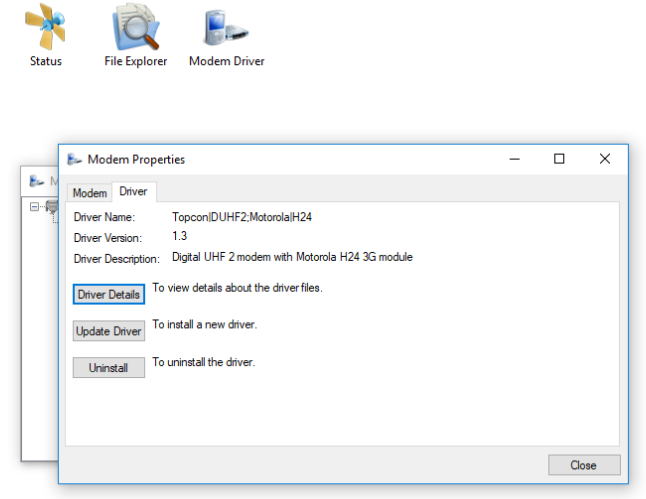
\includegraphics[scale=0.4]{pfc_pdf_files/img/TRU_5_modem.png}
\caption{Configurações de drivers.}
\label{conf_modem_tru}
\end{figure}

Para realizar as configuração das informações de entrada e saída nas portas do receptor deve-se acessar a opção \textit{Receiver Settings} conforme figura \ref{TRU_rec_settings} e em seguida acessar a opção \textit{Ports} conforme figura \ref{TRU_rec_ports}.

\begin{figure}[H]
\centering
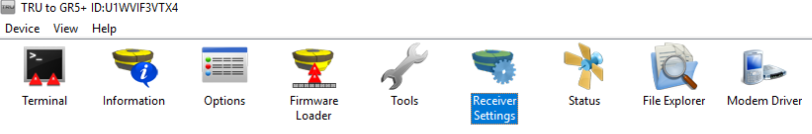
\includegraphics[scale=0.5]{pfc_pdf_files/img/TRU_6_rec_set.png}
\caption{Configurações do receptor.}
\label{TRU_rec_settings}
\end{figure}

\begin{figure}[H]
\centering
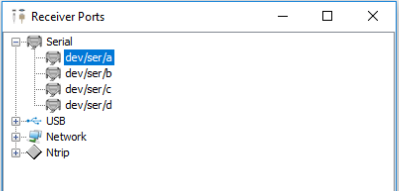
\includegraphics[scale=0.6]{pfc_pdf_files/img/TRU_7_rec_ports.png}
\caption{Configurações das portas do receptor.}
\label{TRU_rec_ports}
\end{figure}

A porta que realiza a comunicação de dados com o BNC nesse trabalho foi a porta ''dev/ser/a''. Abre-se a configuração dessa porta e seleciona-se o \textit{Output mode} para ''RTK RTCM 3.x'' na aba \textit{General}, conforme figura \ref{porta_a}.

\begin{figure}[H]
\centering
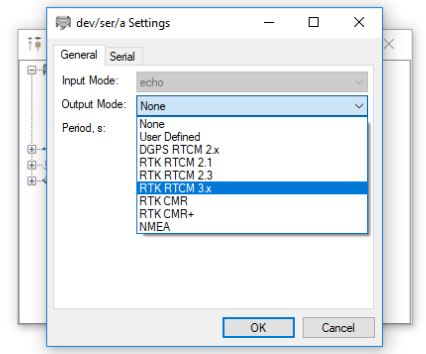
\includegraphics[scale=0.6]{pfc_pdf_files/img/TRU_9_porta_a.png} %scale eh o tamanho que a figura vai ficar
\caption{Formato dos dados de saída.}
\label{porta_a}
\end{figure}

Nessa mesma aba pode-se realizar a verificação das mensagens RTCM que o aparelho está transferindo, conforme figura \ref{msg_receptor}. Por padrão do receptor as mensagens relacionadas as efemérides do sistema GPS e GLONASS (1019 e 1020 respectivamente) não estão incluídas na configuração. Caso ao realizar o RTPPP com o BNC não se conecte ao \textit{stream} \textit{RTCM3EPH} deve-se incluir essas mensagens no aparelho, conforme figura \ref{new_msg_receptor}. Recomenda-se que se conecte ao referido caster utilizando as efemérides recebidas através dele. Ao utilizar as efemérides recebidas pelo próprio receptor nesse trabalho a seguinte mensagem de erro no BNC era transmitida: "\textit{Wrong observation epoch(s)}"

\begin{figure}[H]
\centering
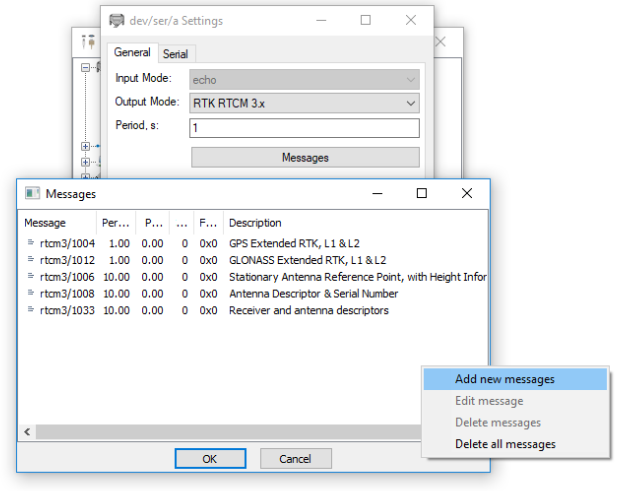
\includegraphics[scale=0.5]{pfc_pdf_files/img/TRU_13_msg.png} %scale eh o tamanho que a figura vai ficar
\caption{Verifica das mensagens transmitidas pelo receptor.}
\label{msg_receptor}
\end{figure}

\begin{figure}[H]
\centering
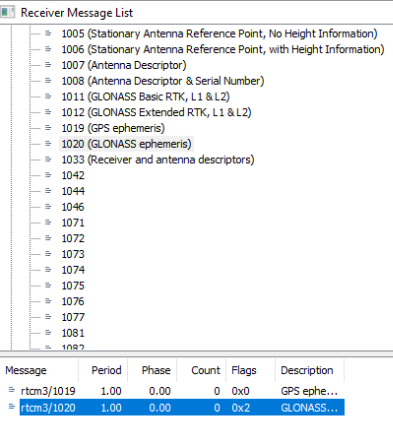
\includegraphics[scale=0.5]{pfc_pdf_files/img/TRU_14_msg.png} %scale eh o tamanho que a figura vai ficar
\caption{Inclusão de novas mensagens para a transmissão.}
\label{new_msg_receptor}
\end{figure}


Na aba \textit{Serial} da mesma janela são realizadas as configurações da transmissão de dados da porta serial. Tais dados devem ser configurados de forma idêntica aos configurados no BNC conforme explicado na seção \ref{rtppp_serial_bnc} e figura \ref{TRU_serial}.

\begin{figure}[H]
\centering
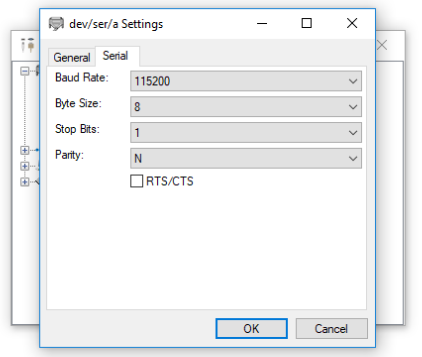
\includegraphics[scale=0.4]{pfc_pdf_files/img/TRU_11_porta_a.png} %scale eh o tamanho que a figura vai ficar
\caption{Configuração de Baud Rate, Byte Size, Stop Bits e Parity.}
\label{TRU_serial}
\end{figure}

O receptor GR-5 armazena os dados do levantamento em cartão de memória SD, nesse trabalho não foi possível acessar os dados gravados diretamente no cartão, para tal foi necessário acessar os dados através do TRU conforme figura \ref{TRU_dados}.

\begin{figure}[H]
\centering
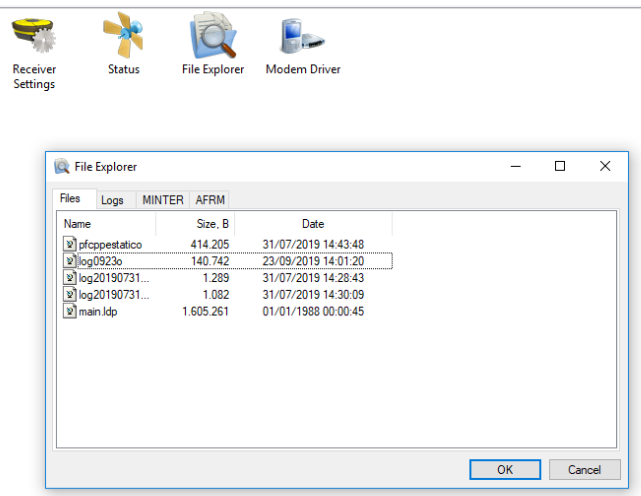
\includegraphics[scale=0.4]{pfc_pdf_files/img/TRU_17_dados.png} %scale eh o tamanho que a figura vai ficar
\caption{Visualização dos arquivos gravados no receptor.}
\label{TRU_dados}
\end{figure}

\section{Configuração do receptor via controladora para realização de RTK}

A fim de realizar as configurações necessárias para a realização de RTK com o receptor GR-5 é interessante a utilização da controladora devido sua portabilidade. A seguir serão descritas algumas configurações básicas a a realização desse método com o GR-5. Cabe ressaltar que caso a comunicação via \textit{bluetooth} entre o receptor e a controladora não esteja funcionando deve-se conectar o receptor ao TRU e alterar a taxa de transmissão da porta "/dev/serial/d'' para 115200.

Após a conexão do receptor com a controladora deve-se abrir a janela ''Configuração'', nomear a configuração e escolher o tipo de método, conforme figura \ref{controladora_conf}.

\begin{figure}[H]
\centering
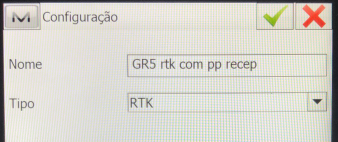
\includegraphics[scale=0.5]{pfc_pdf_files/img/controladora_conf.png} %scale eh o tamanho que a figura vai ficar
\caption{Tela de início para configuração de RTK.}
\label{controladora_conf}
\end{figure}

Escolhe-se o valor para máscara de elevação e o formato para as correções diferenciais enviadas do receptor base para o receptor rover, conforme figura \ref{controladora_cor}

\begin{figure}[H]
\centering
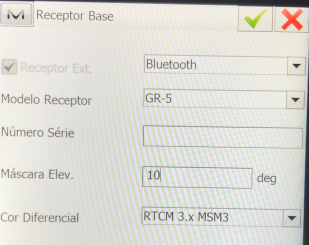
\includegraphics[scale=0.5]{pfc_pdf_files/img/controladora_2.png} %scale eh o tamanho que a figura vai ficar
\caption{Tela correções RTK.}
\label{controladora_cor}
\end{figure}

Escolhe-se onde será feito o armazenamento dos dados, se na controladora ou no receptor conforme figura \ref{controladora_arq}. Recomenda-se que tanto para a Base quanto para o Rover selecione-se "Receptor" visto que nas tentativas realizadas nesse trabalho para arquivamento na controladora os dados não foram armazenados.

\begin{figure}[H]
\centering
\includegraphics[scale=0.5]{pfc_pdf_files/img/controladora_arq.png} %scale eh o tamanho que a figura vai ficar
\caption{Tela de início para configuração de RTK}.
\label{controladora_arq}
\end{figure}

Escolhem-se as configurações de rádio, conforme figuras \ref{controladora_radio} e \ref{controladora_radio2}.

\begin{figure}[H]
\centering
\includegraphics[scale=0.5]{pfc_pdf_files/img/controladora_radio.png} %scale eh o tamanho que a figura vai ficar
\caption{Tela configuração de rádio RTK.}
\label{controladora_radio}
\end{figure}

\begin{figure}[H]
\centering
\includegraphics[scale=0.4]{pfc_pdf_files/img/controladora_radio2.png} %scale eh o tamanho que a figura vai ficar
\caption{Tela 2 configuração de rádio RTK.}
\label{controladora_radio2}
\end{figure}

Realizadas essas configurações as telas se repetirão para determinar as configurações do \textit{rover} que são idênticas a configuração do \texti{base}. As demais telas de configuração são intuitivas.

Após a realização das configurações deve-se iniciar o receptor base, conectar ao receptor rover e então coletar os pontos desejados. 

Cabe ressaltar que para iniciar o receptor base deve-se inserir as coordenadas do ponto em que ele está posicionado ou solicitar que as coordenadas obtidas via GNSS sejam utilizadas. Caso se escolha por inserir as coordenadas manualmente recomenda-se a utilização de coordenadas geográficas visto que nesse trabalho ao utilizar-se de coordenadas cartesianas o sistema trocava as coordenadas X e Y e exibia a mensagem de erro que o receptor estava a mais de 500 metros do ponto informado.





%%
%
% ARQUIVO: apendice.tex
%
% VERSÃO: 1.0
% DATA: Maio de 2016
% AUTOR: Coordenação de Trabalhos Especiais SE/8
% 
%  Arquivo tex de exemplo de apêndice do documento de Projeto de Fim de Curso.
%  Este exemplo traz dois apêndices (dois comandos \chapter{•}). Poderiam ser colocados em arquivos .tex
%  separados. Neste caso, o arquivo main.tex deveria ter um \include{•} para cada arquivo .tex
%
% ---
% DETALHES
%  a. todo apêndice deve começar com \chapter{•}
%  b. usar comando \noindent logo após \chapter{•}
%  c. segue os mesmos DETALHES do arquivo .tex de exemplo de capítulo do documento de Projeto de Fim de Curso
% ---
%%


\chapter{Apêndice B - Códigos}
\noindent

\section{Códigos construídos (Python3) para extração de dados do RTPPP e exibição de gráficos}

Para a extração dos diversos dados obtidos no BNC, PPP-Wizard e IBGE-PPP, \textit{scripts} em linguagem \textit{Python} foram desenvolvidos. A seguir encontram-se esses \textit{scripts}. A explicação detalhada dos códigos encontra-se tanto nos comentários quanto no arquivo ''LEIAME.txt'' dispovível em: <https://github.com/cardosoeng09/real\_time\_ppp>. Nesse link encontra-se todo o projeto, os dados utilizados e arquivos gerados.

\subsection{Código ''main.py''}
\lstinputlisting{data/main.py}


\subsection{Funções auxiliares}
\lstinputlisting{data/graphics.py}

\subsection{Funções para construção dos gráficos e extração dos dados}
\lstinputlisting{data/auxiliary_functions.py}

\section{Extrato do LOG obtido no BNC 2.12 ao realizar RTPPP na estação POAL}

\begin{lstlisting}
19-07-27 00:00:23 2019-07-27_00:00:10.000 POAL00BRA0 X = 3467519.3895 Y = -4300378.7366 Z = -3177517.5357 NEU:  +0.2430  -0.1367  +0.0316 TRP:  +2.3821  +0.0336
19-07-27 00:00:23 2019-07-27_00:00:11.000 POAL00BRA0 X = 3467519.3976 Y = -4300378.7418 Z = -3177517.5480 NEU:  +0.2369  -0.1336  +0.0458 TRP:  +2.3821  +0.0336
19-07-27 00:00:23 2019-07-27_00:00:12.000 POAL00BRA0 X = 3467519.3928 Y = -4300378.7414 Z = -3177517.5469 NEU:  +0.2361  -0.1372  +0.0423 TRP:  +2.3821  +0.0336
19-07-27 00:00:23 2019-07-27_00:00:13.000 POAL00BRA0 X = 3467519.3987 Y = -4300378.7494 Z = -3177517.5474 NEU:  +0.2407  -0.1375  +0.0511 TRP:  +2.3821  +0.0336
19-07-27 00:00:23 2019-07-27_00:00:14.000 POAL00BRA0 X = 3467519.3960 Y = -4300378.7405 Z = -3177517.5460 NEU:  +0.2376  -0.1341  +0.0429 TRP:  +2.3821  +0.0336
19-07-27 00:00:29 2019-07-27_00:00:15.000 POAL00BRA0 X = 3467519.3999 Y = -4300378.7434 Z = -3177517.5477 NEU:  +0.2385  -0.1329  +0.0479 TRP:  +2.3821  +0.0336
\end{lstlisting}
\section{Arquivo de coordenadas da estação POAL para realização de RTPPP com software BNC}
\lstinputlisting{BNC/CONFIG/POA/coordenadas_poa.txt}







\chapter{Apêndice C - Dificuldades}
\noindent

\section{Dificuldades enfrentadas o longo do projeto}

\begin{itemize}
    \item \textit{Porta COM}: Os notebooks mais modernos não possuem entrada COM e a conexão do receptor é por meio desta. Assim, necessitou-se buscar um adaptador COM para USB;
    \item \textit{Atualização de firmware}: A empresa responsável pelo produto veio ao IME realizar a atualização de firmware dos receptores para a correta configuração dos mesmos;
    \item \textit{Configurações da conexão}: Para a correta comunicação do receptor e o notebook, foram necessárias realizar diversas configurações, as quais foram retiradas do manual do GR-5 e testadas. A taxa de transmissão dos dados é uma seleção crucial para ocorrer a comunicação e dentre as opções, apenas uma era a correta;
    \item \textit{Bluetooth}: Ao alterar a taxa de transmissão de dados inúmeras vezes, alteramos a configuração do bluetooth, o qual permite a comunicação entre a Base e o Rover. Para correção, foi preciso investigar o manual e consultas web;
    \item \textit{Mensagem de ''Wrong Epoch''}: Ocorreram divergências entre o horário padrão software BNC e das mensagens advinda dos casters e estações. Ao buscar a solução desse problema, descobriu-se que o BNC possui uma diferença de quatro horas ao fuso padrão do notebook;
    \item \textit{PPP-Wizard}: Pela característica nativa da modificação do BNC pelo código fonte, ocorreram dificuldades no manuseio dessa funcionalidade pela janela de comando, demandando tempo e configurações adicionais.
    
    

\end{itemize}
%\include{caps/capX-anotacoes}
% -----
% PARTE DE REFERÊCIAS BIBLIOGRÁFICAS DE PFC
%
%  As referências do documento de PFC devem estar no arquivo refs.bib
%  Devem seguir o formato bibtex - ver Manual-Referencias.pdf para mais detalhes.
% -----
\bibliographystyle{pfc}
\bibliography{refs}

% -----
% PARTE DE APÊNDICE DE PFC
%
%  Se o documento de PFC não tiver apêndices REMOVER AS LINHAS ABAIXO
%  Adicionar os arquivos .tex de apêndice ao documento com comando \include{•}
% -----
%\inappendix
%%%
%
% ARQUIVO: apendice.tex
%
% VERSÃO: 1.0
% DATA: Maio de 2016
% AUTOR: Coordenação de Trabalhos Especiais SE/8
% 
%  Arquivo tex de exemplo de apêndice do documento de Projeto de Fim de Curso.
%  Este exemplo traz dois apêndices (dois comandos \chapter{•}). Poderiam ser colocados em arquivos .tex
%  separados. Neste caso, o arquivo main.tex deveria ter um \include{•} para cada arquivo .tex
%
% ---
% DETALHES
%  a. todo apêndice deve começar com \chapter{•}
%  b. usar comando \noindent logo após \chapter{•}
%  c. segue os mesmos DETALHES do arquivo .tex de exemplo de capítulo do documento de Projeto de Fim de Curso
% ---
%%


\chapter{Apêndice}
\noindent


\section{Configurações Receptor via porta serial no BNC}

\begin{figure}[H]
\centering
\includegraphics[scale=0.4]{img/18bnc.png} %scale eh o tamanho que a figura vai ficar
\caption{Seleção do receptor como Caster via portal serial.}
\label{Rotulo}
\end{figure}


\begin{figure}[H]
\centering
\includegraphics[scale=0.4]{img/19bnc.png} %scale eh o tamanho que a figura vai ficar
\caption{Configurações do receptor.}
\label{Rotulo}
\end{figure}


\begin{figure}[H]
\centering
\includegraphics[scale=0.4]{img/21bnc.png} %scale eh o tamanho que a figura vai ficar
\caption{Chegada de dados do receptor para o BNC.}
\label{Rotulo}
\end{figure}






\section{Configurações de comunicação entre Receptor e Notebook via software TRU}

\begin{figure}[H]
\centering
\includegraphics[scale=0.4]{img/2.png} %scale eh o tamanho que a figura vai ficar
\caption{Identificação da conexão do receptor via porta serial.}
\label{Rotulo}
\end{figure}


\begin{figure}[H]
\centering
\includegraphics[scale=0.4]{img/3.png} %scale eh o tamanho que a figura vai ficar
\caption{Seleção e atribuição da porta serial ao receptor e conexão.}
\label{Rotulo}
\end{figure}


\begin{figure}[H]
\centering
\includegraphics[scale=0.4]{img/4.png} %scale eh o tamanho que a figura vai ficar
\caption{Configurações de drivers.}
\label{Rotulo}
\end{figure}


\begin{figure}[H]
\centering
\includegraphics[scale=0.4]{img/5.png} %scale eh o tamanho que a figura vai ficar
\caption{Atualização de drivers}
\label{Rotulo}
\end{figure}

\begin{figure}[H]
\centering
\includegraphics[scale=0.4]{img/6.png} %scale eh o tamanho que a figura vai ficar
\caption{Configurações do receptor.}
\label{Rotulo}
\end{figure}


\begin{figure}[H]
\centering
\includegraphics[scale=0.4]{img/9.png} %scale eh o tamanho que a figura vai ficar
\caption{Formato dos dados de saída.}
\label{Rotulo}
\end{figure}

\begin{figure}[H]
\centering
\includegraphics[scale=0.4]{img/9.png} %scale eh o tamanho que a figura vai ficar
\caption{Configuração de Baud Rate, Byte Size, Stop Bits e Parity.}
\label{Rotulo}
\end{figure}


\begin{figure}[H]
\centering
\includegraphics[scale=0.4]{img/11.png} %scale eh o tamanho que a figura vai ficar
\caption{Configuração de Baud Rate, Byte Size, Stop Bits e Parity.}
\label{Rotulo}
\end{figure}

\begin{figure}[H]
\centering
\includegraphics[scale=0.4]{img/13.png} %scale eh o tamanho que a figura vai ficar
\caption{Seleção das mensagens de chegada no receptor.}
\label{Rotulo}
\end{figure}

\begin{figure}[H]
\centering
\includegraphics[scale=0.4]{img/14.png} %scale eh o tamanho que a figura vai ficar
\caption{Seleção das mensagens de chegada no receptor.}
\label{Rotulo}
\end{figure}

\begin{figure}[H]
\centering
\includegraphics[scale=0.4]{img/15.png} %scale eh o tamanho que a figura vai ficar
\caption{Seleção das mensagens de chegada no receptor.}
\label{Rotulo}
\end{figure}

\begin{figure}[H]
\centering
\includegraphics[scale=0.4]{img/17.png} %scale eh o tamanho que a figura vai ficar
\caption{ Visualização de arquivos log.}
\label{Rotulo}
\end{figure}


\section{Códigos construídos (Python3) para extração de dados do RTPPP e exibição de gráficos}
\subsection{Código ''main.py''}
\lstinputlisting{data/main.py}

\subsection{Funções auxiliares}
\lstinputlisting{data/graphics.py}

\subsection{Funções para construção dos gráficos e extração dos dados}
\lstinputlisting{data/auxiliary_functions.py}


\section{Extrato do LOG obtido no BNC 2.12 ao realizar RTPPP na estação POAL}

\begin{lstlisting}
19-07-27 00:00:23 2019-07-27_00:00:10.000 POAL00BRA0 X = 3467519.3895 Y = -4300378.7366 Z = -3177517.5357 NEU:  +0.2430  -0.1367  +0.0316 TRP:  +2.3821  +0.0336
19-07-27 00:00:23 2019-07-27_00:00:11.000 POAL00BRA0 X = 3467519.3976 Y = -4300378.7418 Z = -3177517.5480 NEU:  +0.2369  -0.1336  +0.0458 TRP:  +2.3821  +0.0336
19-07-27 00:00:23 2019-07-27_00:00:12.000 POAL00BRA0 X = 3467519.3928 Y = -4300378.7414 Z = -3177517.5469 NEU:  +0.2361  -0.1372  +0.0423 TRP:  +2.3821  +0.0336
19-07-27 00:00:23 2019-07-27_00:00:13.000 POAL00BRA0 X = 3467519.3987 Y = -4300378.7494 Z = -3177517.5474 NEU:  +0.2407  -0.1375  +0.0511 TRP:  +2.3821  +0.0336
19-07-27 00:00:23 2019-07-27_00:00:14.000 POAL00BRA0 X = 3467519.3960 Y = -4300378.7405 Z = -3177517.5460 NEU:  +0.2376  -0.1341  +0.0429 TRP:  +2.3821  +0.0336
19-07-27 00:00:29 2019-07-27_00:00:15.000 POAL00BRA0 X = 3467519.3999 Y = -4300378.7434 Z = -3177517.5477 NEU:  +0.2385  -0.1329  +0.0479 TRP:  +2.3821  +0.0336
19-07-27 00:00:29 2019-07-27_00:00:16.000 POAL00BRA0 X = 3467519.3985 Y = -4300378.7423 Z = -3177517.5495 NEU:  +0.2361  -0.1332  +0.0473 TRP:  +2.3821  +0.0336
19-07-27 00:00:29 2019-07-27_00:00:17.000 POAL00BRA0 X = 3467519.4080 Y = -4300378.7514 Z = -3177517.5514 NEU:  +0.2410  -0.1316  +0.0595 TRP:  +2.3821  +0.0336
19-07-27 00:00:29 2019-07-27_00:00:18.000 POAL00BRA0 X = 3467519.4062 Y = -4300378.7469 Z = -3177517.5530 NEU:  +0.2373  -0.1302  +0.0564 TRP:  +2.3821  +0.0336
19-07-27 00:00:29 2019-07-27_00:00:19.000 POAL00BRA0 X = 3467519.3978 Y = -4300378.7404 Z = -3177517.5431 NEU:  +0.2406  -0.1326  +0.0424 TRP:  +2.3821  +0.0336
19-07-27 00:00:34 2019-07-27_00:00:20.000 POAL00BRA0 X = 3467519.3852 Y = -4300378.7235 Z = -3177517.5396 NEU:  +0.2331  -0.1318  +0.0224 TRP:  +2.3821  +0.0336
19-07-27 00:00:34 2019-07-27_00:00:21.000 POAL00BRA0 X = 3467519.3970 Y = -4300378.7415 Z = -3177517.5496 NEU:  +0.2352  -0.1339  +0.0460 TRP:  +2.3821  +0.0336
19-07-27 00:00:34 2019-07-27_00:00:22.000 POAL00BRA0 X = 3467519.4080 Y = -4300378.7424 Z = -3177517.5555 NEU:  +0.2339  -0.1260  +0.0555 TRP:  +2.3821  +0.0336
19-07-27 00:00:34 2019-07-27_00:00:23.000 POAL00BRA0 X = 3467519.3999 Y = -4300378.7319 Z = -3177517.5484 NEU:  +0.2334  -0.1257  +0.0405 TRP:  +2.3821  +0.0336
19-07-27 00:00:34 2019-07-27_00:00:24.000 POAL00BRA0 X = 3467519.4032 Y = -4300378.7340 Z = -3177517.5499 NEU:  +0.2339  -0.1244  +0.0445 TRP:  +2.3821  +0.0336
19-07-27 00:00:38 2019-07-27_00:00:25.000 POAL00BRA0 X = 3467519.3932 Y = -4300378.7370 Z = -3177517.5502 NEU:  +0.2317  -0.1341  +0.0412 TRP:  +2.3821  +0.0336
19-07-27 00:00:38 2019-07-27_00:00:26.000 POAL00BRA0 X = 3467519.3946 Y = -4300378.7278 Z = -3177517.5459 NEU:  +0.2323  -0.1272  +0.0336 TRP:  +2.3821  +0.0336
19-07-27 00:00:38 2019-07-27_00:00:27.000 POAL00BRA0 X = 3467519.3969 Y = -4300378.7290 Z = -3177517.5462 NEU:  +0.2333  -0.1261  +0.0358 TRP:  +2.3821  +0.0335
19-07-27 00:00:38 2019-07-27_00:00:28.000 POAL00BRA0 X = 3467519.4109 Y = -4300378.7383 Z = -3177517.5521 NEU:  +0.2362  -0.1211  +0.0526 TRP:  +2.3821  +0.0335
19-07-27 00:00:38 2019-07-27_00:00:29.000 POAL00BRA0 X = 3467519.4076 Y = -4300378.7349 Z = -3177517.5535 NEU:  +0.2326  -0.1216  +0.0493 TRP:  +2.3821  +0.0335
19-07-27 00:00:43 2019-07-27_00:00:30.000 POAL00BRA0 X = 3467519.3959 Y = -4300378.7388 Z = -3177517.5452 NEU:  +0.2377  -0.1331  +0.0414 TRP:  +2.3821  +0.0335
\end{lstlisting}
\section{Arquivo de coordenadas da estação POAL para realização de RTPPP com software BNC}
\begin{lstlisting}
        POAL00BRA0  3467519.4343  -4300378.65881  -3177517.52227  0.0000  0.0000  0.0010 TRM115000.00    NONE TRIMBLE NETR9
 \end{lstlisting}
%\outappendix

% -----
% PARTE DE ANEXO DE PFC
%
%  Se o documento de PFC não tiver anexos REMOVER AS LINHAS ABAIXO
%  Adicionar os arquivos .tex de anexo ao documento com comando \include{•}
% -----
%\inannex
%%%
%
% ARQUIVO: anexo.tex
%
% VERSÃO: 1.0
% DATA: Maio de 2016
% AUTOR: Coordenação de Trabalhos Especiais SE/8
% 
%  Arquivo tex de exemplo de anexo do documento de Projeto de Fim de Curso.
%  Este exemplo traz dois anexos (dois comandos \chapter{•}). Poderiam ser colocados em arquivos .tex
%  separados. Neste caso, o arquivo main.tex deveria ter um \include{•} para cada arquivo .tex
%
% ---
% DETALHES
%  a. todo anexo deve começar com \chapter{•}
%  b. usar comando \noindent logo após \chapter{•}
%  c. segue os mesmos DETALHES do arquivo .tex de exemplo de capítulo do documento de Projeto de Fim de Curso
% ---
%%
\chapter{Anexo Exemplo}
\noindent
Id magna feugiat. Erat pellentesque sapien in rhoncus dolor augue vel eget. Erat nibh animi ultricies sit rhoncus. Eleifend aliquam luctus sem turpis habitasse. Lectus arcu ut mi nulla luctus facilisis cursus suspendisse class sociis metus vitae leo consequat lorem ullamcorper arcu. Nunc justo aliquam. Quidem volutpat urna. Nonummy nulla blandit donec vitae ultrices. Netus aliquam vivamus. Vehicula libero leo. Vestibulum consectetuer magna. Sapien aliquam arcu netus etiam lectus. Venenatis tristique morbi non nulla tortor commodo gravida ac neque lacinia urna. Elit mauris adipisci. Vitae sed curabitur. Tellus nunc lectus. Nonummy et integer.

Lorem dictumst enim. Dui vestibulum quisque. Dolor posuere risus. Nullam vitae est magnis est tortor metus dolor integer. Massa elit nec euismod et lacus quam ac malesuada est suspendisse ut est pellentesque vivamus lorem amet non vulputate maecenas et id ultrices lacus odio morbi vitae ac aenean in feugiat elit sodales congue proin dui leo bibendum scelerisque faucibus in suscipit. Nulla parturient in. Eget habitasse fringilla. Eget donec excepturi wisi lorem lacinia. Elementum lorem sem. Pede metus sit. Aenean facilisi pellentesque. Purus dictum ante. Neque amet sed.

Sed leo molestie. Elit fusce placerat lectus quis aliquam nulla turpis platea. Integer mus bibendum sed wisi pretium ullamcorper nunc arcu. Ipsum maecenas sed. Et pariatur in. Ut wisi non. Bibendum nec et quisque quam diam sed dolor lorem. Pellentesque fames donec senectus nulla purus dui nibh praesent. Pariatur nulla augue sapien elit imperdiet aliquam ullamcorper orci. Integer nec mauris. Sit magnis vel ut leo a sapien proin at. Etiam sem aliquam bibendum mauris purus ac sagittis ultrices. Mollis eleifend est. Nec vitae posuere at arcu purus. In elementum vehicula.

\chapter{Anexo Exemplo 02}
\noindent
Id magna feugiat. Erat pellentesque sapien in rhoncus dolor augue vel eget. Erat nibh animi ultricies sit rhoncus. Eleifend aliquam luctus sem turpis habitasse. Lectus arcu ut mi nulla luctus facilisis cursus suspendisse class sociis metus vitae leo consequat lorem ullamcorper arcu. Nunc justo aliquam. Quidem volutpat urna. Nonummy nulla blandit donec vitae ultrices. Netus aliquam vivamus. Vehicula libero leo. Vestibulum consectetuer magna. Sapien aliquam arcu netus etiam lectus. Venenatis tristique morbi non nulla tortor commodo gravida ac neque lacinia urna. Elit mauris adipisci. Vitae sed curabitur. Tellus nunc lectus. Nonummy et integer.

Lorem dictumst enim. Dui vestibulum quisque. Dolor posuere risus. Nullam vitae est magnis est tortor metus dolor integer. Massa elit nec euismod et lacus quam ac malesuada est suspendisse ut est pellentesque vivamus lorem amet non vulputate maecenas et id ultrices lacus odio morbi vitae ac aenean in feugiat elit sodales congue proin dui leo bibendum scelerisque faucibus in suscipit. Nulla parturient in. Eget habitasse fringilla. Eget donec excepturi wisi lorem lacinia. Elementum lorem sem. Pede metus sit. Aenean facilisi pellentesque. Purus dictum ante. Neque amet sed.

Sed leo molestie. Elit fusce placerat lectus quis aliquam nulla turpis platea. Integer mus bibendum sed wisi pretium ullamcorper nunc arcu. Ipsum maecenas sed. Et pariatur in. Ut wisi non. Bibendum nec et quisque quam diam sed dolor lorem. Pellentesque fames donec senectus nulla purus dui nibh praesent. Pariatur nulla augue sapien elit imperdiet aliquam ullamcorper orci. Integer nec mauris. Sit magnis vel ut leo a sapien proin at. Etiam sem aliquam bibendum mauris purus ac sagittis ultrices. Mollis eleifend est. Nec vitae posuere at arcu purus. In elementum vehicula.

%\outannex

% -----
% FIM DO DOCUMENTO DE PFC
% -----
\label{theend}
\end{document}
